%% 
%% This is a sample doctoral dissertation.  It shows the appropriate
%% structure for your dissertation.  It should handle most of the
%% strange requirements imposed by the Grad school; like the different
%% handling of titles of one/many appendices.  It will automatically
%% handle the linespacing changes.  The body default is double-spaced
%% (except when you use the singlespace or condensed options).  The
%% default for quotations is single-space, and the default for tabular
%% environments is also single-space.  
%%
%% This class adds the following commands and environments to the
%% report class, upon which it is based:
%% Commands
%% ------------
%% \degree{name}{abbrv} -- Sets the name and abbreviation for the degree.
%%                         These default to ``Doctor of Philosopy''
%%                         and ``Ph.D.'', respectively.
%% \copyrightyear{year} -- for the copyright page.
%% \bachelors{degree}{institution} -- for the abstract
%% \masters{degree}{institution}   --  "
%%     if you have other degrees you may use
%% \secondbachelors{degree}{institution}
%% \thirdbachelors{degree}{institution}
%% \secondmasters{degree}{institution}
%% \thirdmasters{degree}{institution}
%% \priordoctorate{degree}{institution}
%%
%% \committeechair{name}           -- for the signature page
%% or, if you have two co-chairs:
%% \cochairs{first name}{second name}
%%
%% \firstreader{name}              --  "
%% \secondreader{name}             --  "
%% \thirdreader{name}              -- (optional)
%% \fourthreader{name}             --  "
%% \fifthreader{name}              --  "
%% \sixthreader{name}              --  "
%% \departmentchair{name}          -- for the signature page
%% \departmentname{name}           --  "
%%
%% \copyrightpage                  -- produces the copyright page
%% \signaturepage                  -- produces the signature page
%%
%% \frontmatter                    -- these are required in their various
%% \mainmatter                     -- appropriate locations
%% \backmatter                     --
%%
%% \unnumberedchapter[toc]{name}   -- like \chapter, except that it
%%                                    produces an unnumbered chapter;
%%                                    alternatively, like \chapter*,
%%                                    except that it lists the chapter
%%                                    in the table of contents.
%%
%% New environments:
%%   dedication  -- for the dedication
%%   abstract    -- for the abstract
%%
%% The thesis documentclass is built on top of the report document class.
%% It accepts all of the options that the report class accepts, plus the
%% following:
%%     doublespace -- the default, indicates double spacing as per U.Mass.
%%                    requirements.  You will need this when you do your
%%                    final copy.
%%     singlespace -- for earlier work, not acceptable to the Grad school
%%     condensed   -- for earlier work, not acceptable to the Grad school,
%%                    creates condensed versions of the frontmatter. 
%%                    Condensed implies singlespace.
%%     dissertation - the default, indicates that this document is a
%%                    dissertation.
%%     proposal    -- indicates that this document is a dissertation proposal,
%%                    rather than a dissertation.  This will only change the
%%                    wording on the title and signature pages.
%%     thesis      -- indicates that this document is a Master's thesis 
%%                    rather than a doctoral dissertation.  This also changes
%%                    the default for \degree to Master of Science, M.S.
%%     allowlisthypenation -- (the default), allows hyphenation of words in
%%                    the table of contents, the list of figures, and the list
%%                    of tables.  I believe that this is acceptable to the 
%%                    Graduate School.
%%     nolisthyphenation -- disallows hyphenation of words in the table of
%%                    contents and the list of figures and tables.  Use this 
%%                    option if the Grad School doesn't like your hyphenation.
%%     nicerdraft  -- relaxes some of the Grad School's rules for working with
%%                    drafts -- has no effect when doublespace is in effect
%%     nonicerdraft -- the default, leaves things in draft as they will be in
%%                     the final version
%% umthesis changes the default font size to 12pt, but you may specify 10pt or
%%   11pt in the options.
%%\documentclass[proposal]{umthesis}          % for Ph.D. dissertation or proposal
\documentclass{umthesis}          % for Ph.D. dissertation or proposal
%\documentclass{umthesis}          % for Ph.D. dissertation or proposal
% \documentclass[thesis]{umthesis}  % for Master's thesis

\usepackage{color}
\usepackage{listings}
\usepackage{amsmath}
\usepackage{amsfonts}
\usepackage{amssymb}
\usepackage{comment}
\usepackage{graphicx, subfigure}
\usepackage{url}
\usepackage{pifont}% http://ctan.org/pkg/pifont

%\lstset{ %
% language=C,                    % choose the language of the code
% basicstyle=\footnotesize,       % the size of the fonts that are used for the code
%numbers=left,                   % where to put the line-numbers
%numberstyle=\footnotesize,      % the size of the fonts that are used for the line-numbers
%stepnumber=1,                   % the step between two line-numbers. If it is 1 each line will be numbered
%numbersep=5pt,                  % how far the line-numbers are from the code
%backgroundcolor=\color{white},  % choose the background color. You must add \usepackage{color}
%showspaces=false,               % show spaces adding particular underscores
%showstringspaces=false,         % underline spaces within strings
%showtabs=false,                 % show tabs within strings adding particular underscores
%frame=single,           % adds a frame around the code
%tabsize=2,          % sets default tabsize to 2 spaces
%captionpos=b,           % sets the caption-position to bottom
%breaklines=true,        % sets automatic line breaking
%breakatwhitespace=false    % sets if automatic breaks should only happen at whitespace
%escapeinside={\%*}{*)}          % if you want to add a comment within your code
%}

%%
%% If you have enough figures or tables that you run out of space for their
%% numbers in the List of Tables or List of figures, you can use the following
%% command to adjust the space left for numbers.  The default is shown:
%%
%% \setlength{\tablenumberwidth}{2.3em}
\newcommand{\dthreads}{{\scshape Dthreads}}
\newcommand{\Dthreads}{{\scshape Dthreads}}
\newcommand{\Grace}{{\scshape Grace}}
\newcommand{\grace}{{\scshape Grace}}
\newcommand{\Sheriff}{{\scshape Sheriff}}
\newcommand{\sheriff}{{\scshape Sheriff}}
\newcommand{\SheriffProtect}{\textsc{Sheriff-Protect}}
\newcommand{\sheriffProtect}{\textsc{Sheriff-Protect}}
\newcommand{\sheriffprotect}{\textsc{Sheriff-Protect}}
\newcommand{\SheriffDetect}{\textsc{Sheriff-Detect}}
\newcommand{\sheriffDetect}{\textsc{Sheriff-Detect}}
\newcommand{\Predator}{\textsc{Predator}}
\newcommand{\predator}{\textsc{Predator}}
\newcommand{\DoubleTake}{\textsc{DoubleTake}}
\newcommand{\doubletake}{\textsc{DoubleTake}}
\newcommand{\pthreads}{\texttt{pthreads}}
\newcommand{\cmark}{\ding{52}} %51 or 52
\newcommand{\xmark}{\ding{53}}% 53, 54, 55, 56


\begin{document}

%%
%% You must fill in all of these appropriately
\title{Safe and Efficient Multithreading}
\author{Tongping Liu}
\date{January 2013} % The date you'll actually graduate -- must be
                     % February, May, or September
\copyrightyear{2013}
\bachelors{B.S.}{Harbin Institute of Technology}
\masters{M.E.}{Huazhong University of Science and Technology}
\secondmasters{M.S.}{UNIVERSITY OF MASSACHUSETTS AMHERST}
\priordoctorate{Ph.D.}{UNIVERSITY OF MASSACHUSETTS AMHERST}
\committeechair{Emery D. Berger}
\firstreader{Scott F. H. Kaplan}
\secondreader{Yuriy Brun}
\thirdreader{Israel Koren}   % Optional
%\fifthreader{}            % Optional
%\sixthreader{}            % Optional
\departmentchair{Lori A. Clarke}
\departmentname{Department of Computer Science}

%% If your degree is something other than a Ph.D. (for a dissertation), or
%% an M.S. (for a thesis), you will need to uncomment the appropriate
%% following line:
%%
%% \degree{Doctor of Education}{Ed.D.}
%% \degree{Doctor of Philosophy}{Ph.D.}
%%
%% \degree{Master of Arts}{M.A.}
%% \degree{Master of Arts in Teaching}{M.A.T.}
%% \degree{Master of Business Administration}{M.B.A.}
%% \degree{Master of Education}{M.Ed.}
%% \degree{Master of Fine Arts}{M.F.A.}
%% \degree{Master of Landscape Architecture}{M.L.A.}
%% \degree{Master of Music}{M.M.}
%% \degree{Master of Public Administration}{M.P.A.}
%%\degree{Master of Public Health}{M.P.H.}
%% \degree{Master of Regional Planning}{M.R.P.}
%% \degree{Master of Science}{M.S.}
%% \degree{Master of Science in Accounting}{M.S. Acctg.}
%% \degree{Master of Science in Chemical Engineering}{M.S. Ch.E.}
%% \degree{Master of Science in Civil Engineering}{M.S.C.E.}
%% \degree{Master of Science in Electrical and Computer Engineering}{M.S.E.C.E.}
%% \degree{Master of Science in Engineering Management}{M.S. Eng. Mgt.}
%% \degree{Master of Science in Environmental Engineering}{M.S. Env. E.}
%% \degree{Master of Science in Industrial Engineering and Operations Research}{M.S.I.E.O.R.}
%% \degree{Master of Science in Manufacturing Engineering}{M.S. Mfg. Eng.}
%% \degree{Master of Science in Mechanical Engineering}{M.S.M.E.}
%%
%% \degree{Professional Master of Business Administration}{P.M.B.A.}


%%
%% These lines produce the title, copyright, and signature pages.
%% They are Mandatory; except that you could leave out the copyright page
%% if you were preparing an M.S. thesis instead of a PhD dissertation.
\frontmatter
\maketitle
\copyrightpage     %% not required for an M.S. thesis
\signaturepage

%%
%% Dedication is optional -- but this is how you create it
%\begin{dedication}              % Dedication page
%  \begin{center}
%   \emph{ XXXXXX }       
%  \end{center}
%\end{dedication}

%%
%% Epigraph goes here...(aka frontispiece)
%% \chapter{Epigraph}?????

%%
%% Acknowledgements are optional...yeah, right.
%  \chapter{Acknowledgments}             % Acknowledgements page
%  Thanks to all those fine shepherds. Not to mention all the great
%  border collies and suchlike fine animals.

%%
%% Abstract is MANDATORY. -- Except for MS theses

\begin{abstract}                % Abstract
The advent of multicore architecture has increased the demand for multithreaded
programs, but writing them remains painful for programmers. 
It is notoriously far more challenging to write concurrent programs correctly and 
efficiently than sequential ones because of the wide range of performance problems and 
concurrency errors, including false sharing, race conditions, deadlocks, etc. 

In this proposal we introduce a series of runtime systems to combat performance problems and 
concurrency errors of multithreaded problems.
The first system, \Sheriff{}, attacks the notorious performance problem of 
multithreaded programs, false sharing. \Sheriff{} can precisely detect false 
sharing problems without false positives and automatically mitigate false sharing 
problems without user intervention. 
The second system, \dthreads{}, automatically ensures determinism for unmodified C/C++
applications without requiring programmer intervention. \dthreads{} leverages virtual 
memory and process isolation, combined with a deterministic commit protocol, 
to ensure robust deterministic execution with very low runtime overhead.
Finally, we propose \DoubleTake{}, a novel detection tool for write-write races based on synchronization
 boundaries.
\DoubleTake{} detects more races than the standard happens-before
approaches without introducing false positives, unlike lockset based approaches.
\DoubleTake{} can also locate those heap-based overflows and 
underflows without adding perceptible performance overhead.

\end{abstract}

%%
%% Preface goes here...would be just like Acknowledgements -- optional
%% \chapter{Preface} 
%% ...


%%
%% Table of contents is mandatory, lists of tables and figures are 
%% mandatory if you have any tables or figures; must be in this order.
\tableofcontents                % Table of contents
%\listoftables                   % List of Tables
\listoffigures                  % List of Figures

%%
%% We don't handle List of Abbreviations
%% We don't handle Glossary

%%%%%%%%%%%%%%%%%%%%%%%%%%%%%%%%%%%%%%%%%%%%%%%%%%%%%%%%%%%%%%%%%%%%%%%%%
%% Time for the body of the dissertation
\mainmatter   %% <-- This line is mandatory

%%
%% If you want an introduction, which is not a numbered chapter, insert
%% the following two lines.  This is OPTIONAL:
\unnumberedchapter{Introduction}
For decades, applications enjoyed automatic and regular performance gains from increasingly faster CPU speed.  However, this trend has stopped permanently because of hard physical limits. Increasing CPU speed results in consuming more energy and generating more heat. Intel and other vendors have turned to providing more and more cores on a single machine, which brings us the multi-core era. The appearance of multi-core drives the biggest revolution multithreaded programs of software development: software has to be programmed in a concurrent and parallel way in order to exploit the benefits of multi-core machines.

Building efficient and reliable concurrent software is still a challenging task because of the following reasons. First, concurrency requires programmers to think in an unnatural way that humans find difficult.  Second, existing languages and tools are inadequate to detect or prevent concurrency errors and performance anomalies. 

% Why we need determinism? Concurrency errors?
Concurrency errors of multithreaded programs, such as race conditions, atomicity violations, order violations and deadlocks, are very hard to debug ~\cite{Lu:2008:LMC:1346281.1346323}, because their occurrences highly depend on some specific conditions, such as thread interleavings and CPU scheduling ~\cite{DBLP:conf/icse/BallBHMQ09,DBLP:conf/asplos/BurckhardtKMN10}. Instead of detecting possible concurrency errors, one promising alternative approach is to attack the problem of concurrency bugs by eliminating its source: non-determinism. A fully \emph{deterministic multithreading system} would prevent Heisenbugs by ensuring that executions of the same program with the same inputs always yield the same results, even in the face of race conditions in the code. Such a system would not only dramatically simplify debugging of concurrent
programs~\cite{Carver:1991:RTC:624586.625040} and reduce their attendant testing overhead, but would also enable a number of other applications. For example, a deterministic multithreaded system would greatly simplify record-and-replay for multithreaded programs~\cite{Choi:1998:DRJ:281035.281041,LeBlanc:1987:DPP:32387.32396} and the deterministic replication of a multithreaded application on different machines for fault tolerance~\cite{deterministic-process-groups,1134000,224058,replicant-hotos}.

% Why we need to find out false sharing problems.
Besides concurrency errors, writing efficient multithreaded programs remains challenging too. False sharing problem is one of the notorious performance problems inside multithreaded programs~\cite{falseshare:Analysis, falseshare:effect}. It occurs when multiple threads, running on different cores with their separate caches, are accessing logically independent words in the same cache line. If a thread modifies anything inside a cache line, cache coherence protocol invalidates the duplicates of this cache line in other caches in order to guarantee correctness of programs, which is crucial for true sharing cases. However, it is totally unnecessary for false sharing cases. False sharing can force one core to wait unnecessarily for updates from another processor, thus wasting both the CPU time and precious memory bandwidth in the same time. 

\subsection*{Contributions}

This thesis handles two categories of problems inside multithreaded programs, the reliability problem and the performance problem, and makes the following contributions:

\begin{itemize}
\item \Sheriff{} framework: I developed a novel processes-as-threads framework by borrowing the idea from Grace~\cite{grace}. \sheriff{} is a software-only drop-in replacement of the stand \pthreads{} library. It turns threads into processes, with separate address spaces but the shared file table. \sheriff{} provides per-thread memory protection and isolation on page granularity, relying on the stand memory protection mechanism and twining-and-diffing mechanism. \sheriff{} enables a range of possible applications, including language support and enforcement of data sharing, software transactional memory, thread-level speculation, and race detection. 

\item I developed an efficient deterministic multithreading system, \dthreads{}, for unmodified C/C++ applications,  without programmer intervention and hardware support. \dthreads{} is based on the \sheriff{} framework to isolate executions of different threads. \dthreads{} outperforms the previous state-of-the-art runtime system (CoreDet) by a factor of 3, and often matches and sometimes exceeds the performance with the standard \pthreads{} library. \Dthreads{} enforces robust/stable determinism even in the face of data races, greatly simplifying program understanding and debugging: programs always behave the same, even with different inputs and on different hardware, as long as the synchronization order is staying the same. Because of this, \dthreads{} can also be used to support replicated executions of multithreaded applications for fault tolerance purposes.

\item 
Based on the \sheriff{} framework, I developed another two tools, \SheriffDetect{} and \SheriffProtect{}, to deal with false sharing problems of multithreaded programs, one of the notorious performance problems. 
\SheriffDetect{} find instances of false sharing accurately (no false positives), runs with low overhead (on average 20\%), and can precisely pinpoint the exact objects involved in false sharing. \SheriffProtect{} mitigates false sharing problems by adaptively isolating shared accesses on a cache line from different threads into separate physical addresses, effectively eliminating the performance impact of false sharing. It can boost the performance automatically for those multithreaded applications with false sharing problems inside, without the need of programmer intervention. 

\item I also developed a tool, \predator{}, to improve the effectiveness of false sharing detection. Instead of relying on the \sheriff{} framework to track memory writes, \predator{} employs compiler instrumentation to track read and write memory accesses, which make it possible to detect one more type of false sharing, read-write false sharing. \Predator{} also overcomes a key limitation of previous detection tools: existing tools can only detect those observed false sharing problems. However, the occurrences of false sharing highly depend on memory layout and size of a cache line, which are affected by a lot of dynamic properties. \Predator{} can predict potential false sharing that does not manifest in a given execution but may appear---and greatly degrade application performance—--in a slightly different execution environment. \Predator{} is the first false sharing tool able to automatically and precisely uncover false sharing problems in real applications, including MySQL and the Boost library.


\end{itemize}

\subsection*{Outline}
The rest of this thesis is organized as follows. Chapter~\ref{chapter:problems} describes the reliability and performance problems of multithreaded programs, which we are going to handle in this thesis. Chapter~\ref{sec:sheriffframework} describes the processes-as-threads framework, \sheriff{}, which is the basis for \dthreads{}, \SheriffDetect{} and \SheriffProtect{}. Chapter~\ref{chapter:dthreads} describes \dthreads{} that ensures deterministic execution for multithreaded programs linking to this drop-in library. Chapter~\ref{chapter:sherifftools} discusses how to precisely detect and automatically tolerate false sharing problems based on the \sheriff{} framework. Chapter~\ref{chapter:preditor} describes a generalized false sharing detection tool by combining compiler instrumentation and runtime system, which improves the effectiveness of false sharing detection. 
Chapter~\ref{chapter:relatedwork} provides a substantial comparison between previous work and our approaches and Chapter~\ref{chapter:conclusion} concludes the thesis with its contributions and possible future work. 


%%
%% Some sample text



\chapter{Multithreading Problems}
%Sheep are fabulous creatures.  The noises they make are truly stupendous
%\cite{Bah}.  We also want to refer to figure \ref{fig:circle} here.
%Here's some verbatim text to screw us up:
\label{chapter:problems}

Writing Multithreaded programs can encounter concurrency errors and performance anomalies. This thesis discusses in detail two different types of problems, non-determinism and false sharing.  We discuss the definitions, causes of these problems and their possible consequence as follows.

\section{Non-determinism}
\label{sec:nondeterminism}

\subsection{Background}
Deterministic behavior of programs is the most desirable behavior: given the same input, a program
produces the same output and generates the same execution. Relying on this behavior, it is able to figure out problems of programs. 

In reality, it is relatively easy for sequential programs to achieve this target if a program do not explicitly rely on a randomized mechanism. 
However, it is hard to do this for parallel programs. In shared memory multithreaded programs, an application can only experience one of many possible 
schedules at a time. Thread scheduling, the order of memory accesses on the shared data, operations depending on timing and non-deterministic synchronizations, can easily lead to different executions of the same program.


\begin{figure*}[!ht]
{\centering
\fbox{
\subfigure{\lstinputlisting[numbers=none,frame=none,boxpos=t]{fig/nondeter.sample1}}
\hspace{20pt}
\subfigure{\lstinputlisting[numbers=none,frame=none,boxpos=t]{fig/nondeter.sample2}}
\hspace{20pt}
\subfigure{\lstinputlisting[numbers=none,frame=none,boxpos=t]{fig/nondeter.sample3}}
}
\caption{Non-determinism problem 
\label{fig:nondeterminism}}
}
\end{figure*}

A simple example of non-deterministic execution can be seen in Figure~\ref{fig:nondeterminism}. When using the standard \pthreads{} library, this program can print ``1,0'', ``0,1'' or ``1,1'' in the end, depending on the order of memory accesses from different threads. We actually run this simple program for one million times. About 99.43\% of time, it will print ``1,0'', while 0.56\% it will print ``0,1'' and 0.01\% it will print ``1,1''. According to the semantics of this program, both ``1,0'' and ``1,0'' are correct results. Thus, the unexpected result (``1,1'') caused by race conditions happens very rarely, only about 0.01\%.  
It is very difficult to observe/reproduce these rare cases that caused by race conditions.

\subsection{Source of Non-determinism}
Non-determinism can be caused by a lot of sources, both external sources and internal sources. For example, the timing of external inputs is one of the sources that can lead to non-determinism. This section only lists internal sources of non-determnism~\cite{costofdeterminism}. 
 
\emph{Thread Communication}: 
Thread communication is the most important source of non-determinism for multithreaded programs. 
First, the order of accesses on shared variables may change from one execution to the other. Second, the orders on shared resources, such as memory allocation, synchronization, and library/system calls, vary across different executions. 
Third, the interaction between compiler and run-time can be changed. For example, lazy binding may cause the thread that  performs address resolution to execute much more instructions than others. 

\emph{Memory Layout}: 
Address space layout randomization (ASLR) in Linux environment brings non-deterministic memory addresses of instructions and data across different executions. Thus, a program relying on memory addresses lead to non-deterministic execution of a program. 

\emph{System or Library Dependence}:
Some library or system calls cannot return deterministic results. For example, the \texttt{gettimeofday()} library call returns different time values at different time, and \texttt{read} system calls may return different number of bytes, depending on the timing of issuing \texttt{read} calls.  An application relying on them can execute non-deterministically too. 


\subsection{Effect of Non-determinism}
Because of different sources of non-determinism, listed in the above section, existing multithreaded applications can not run deterministically: given the same input, a program can have different executions that may or may not lead to different outputs. 

Non-determinism can greatly complicate the reasoning and debugging in development phases, which makes it hard for programmers to reproduce program errors. 
Even worse, since executions of deployment can vary from executions of development phase, a lot of programmer errors can be easily leaked to customers.

By contrast, determinism greatly simplifies the understanding and debugging of multithreaded programs. We can always guarantee the same executions on both development phases and the deployment phases, thus there is no need to worry about erroneous results. 

\section{False Sharing}
\label{sec:falsesharingproblems}

\subsection{Definition}
% What is the definition of false sharing?
False sharing occurs when different processors in a shared-memory parallel system are referencing distinct fields within the same coherence block (page or cache line) simultaneously, thereby inducing ``unnecessary'' coherence traffic~\cite{Bolosky:1993:FSE:1295480.1295483}. 

Although it is difficult or impossible to know where a thread runs in an actual execution, we can conservatively assume that different threads are running on different processors with separate cache. Thus, in the multithreaded environment, false sharing simply implies: multiple threads access distinct parts of the same cache line simultaneously, while one of them is a write operation. False sharing is shown in Figure~\ref{fig:fs}. 
Based on the relationship of false sharing objects, 
false sharing can be classified into inter-object and intra-object false sharing. When two different objects in the same cache line are accessed by different threads simultaneously, that is inter-object false sharing. Otherwise, it is intra-object false sharing. 

There is another concept, true sharing, which is opposite of false sharing. In true sharing (Figure~\ref{fig:ts}), multiple threads are accessing the same word. 

There is another way to differentiate false sharing with true sharing. False sharing is avoidable, while true sharing is not. 

\begin{figure*}
\begin{center} 
\subfigure[False sharing]{%
   \label{fig:fs}
   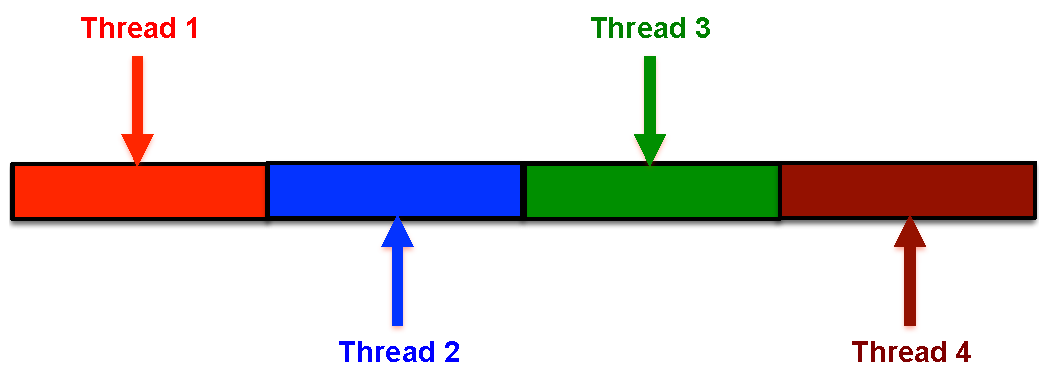
\includegraphics[width=2.4in]{sheriff/figure/falsesharing.pdf}
}%
\hspace{50pt}
\subfigure[True sharing]{%
   \label{fig:ts}
   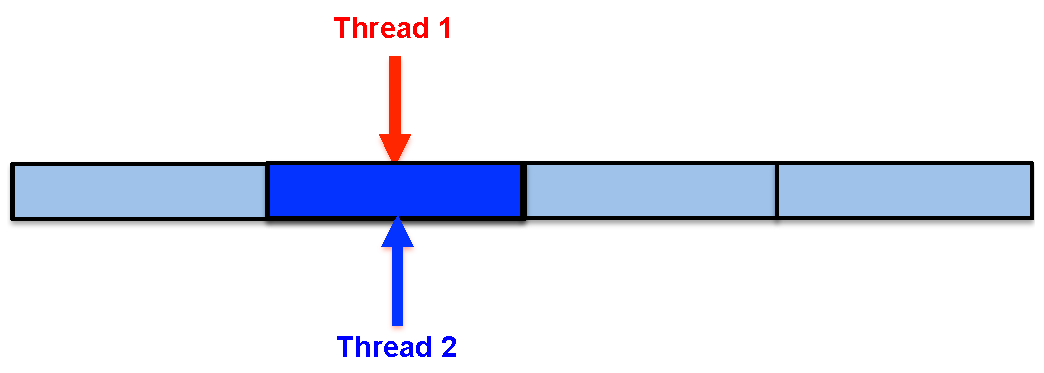
\includegraphics[width=2.4in]{sheriff/figure/truesharing.pdf}
}%
\end{center}
%\includegraphics{fig/potential.pdf}
\caption{False sharing and true sharing in a cache line with four words. }
\label{fig:fsexample}
\end{figure*}

% The classification of false sharing?

\subsection{Reason of False Sharing}

As shown in Figure~\ref{fig:fsexample}, false sharing only occurs when the size of coherence block is larger than that of a single word. Multiple processors may reference different words of the same coherence block. In this perspective, a single-word block size can avoid false sharing problems. 

However, using a single-word block size is not the actual case. In reality, the size of a coherence block (cache line) is normally 32 or 64 bytes. The reason of using multiple words in a cache line is to reduce the groups of transfers between the main memory and the cache since programs always have some spatial locality of reference. Those adjacent words are very likely to be referenced in the future.

From the performance perspective, reducing the coherence block size to one word may minimize the data to transferred, but can increase the number of transfers. Thus, the overhead of transferring less data at a time can be larger than the benefit of eliminating false sharing coherence traffic. Actually, the hardware trend of cache line is to increase the size of cache line, which makes false sharing problems increasingly common. 

\subsection{Performance Impact}
\label{falsesharing}
False sharing can greatly slowdown the execution of multithreaded programs, which depends on many factors, including the cache block size, data layout, program access patterns, and the cost of coherence operations~\cite{Bolosky:1993:FSE:1295480.1295483}. 

In a typical shared-memory system, each processor may have a separate cache. In order to increase the access speed, when a processor references a word, all the data inside the same cache line is fetched from the main memory to its corresponding cache. 
When multiple processors are accessing distinct words of the same cache line simultaneously, the shared data can be replicated into caches of different processors that access this cache line. Thus, it is very important to maintain the coherence across different processors: if any copy is changed, this change should be propagated to other processors immediately for correctness purposes. In real hardware, this data propagation only happens lazily when the data is accessed again, thus duplicates are invalidated at first. When a processor access an invalidated cache line, it should wait for the data propagating from other processors, wasting CPU time and memory bandwidth simultaneously. 

In the false sharing case, this propagation is totally unnecessary because different threads are actually accessing different parts of the same cache line. Thus, there is no need for a processor to get the updated data that is not going to access. However, hardware can only tracks the change of data on the granularity of a cache line and have to propagate those changes if any word has been changed. When there are interleaved writes, issued by different processors, on the same cache line, the ping-pong effect of loading-and-invalidating of data on this cache line can greatly slow the execution of programs. 
Programs with false sharing can even run slower in a multi-core machine than in a single-core machine, losing the benefit of multiple cores.  

Many common programming practices can easily cause false sharing. For example, different threads accessing different entries of the same global array, listed in Figure~\ref{fig:falsesharingexample}, is such an example. This example has no correctness problem, but a serious performance problem. 

\begin{figure*}[!ht]
{\centering
\fbox{
\subfigure{\lstinputlisting[numbers=none,frame=none,boxpos=t]{fig/falsesharing.sample1}}
\hspace{20pt}
\subfigure{\lstinputlisting[numbers=none,frame=none,boxpos=t]{fig/falsesharing.sample2}}
}
\caption{False sharing problem
\label{fig:falsesharingexample}}
}
\end{figure*}

We actually run this program on a real machine with 8 cores and Figure~\ref{fig:fsperfimpact} presents performance results. On this evaluation, we specifically choose a different number of threads, matching the number of hardware cores, from 1 thread to 8 threads, to perform the same amount of workload. We find out that false sharing can greatly impact the performance, which brings around $13\times$ difference between actual performance and the expected performance. Two trends--the prevalence of multicore architectures and
the expected increase in the number of multithreaded applications in broad use, and increasing cache line sizes--are likely to make false sharing increasingly common.

\begin{figure*}[!t]
\centering
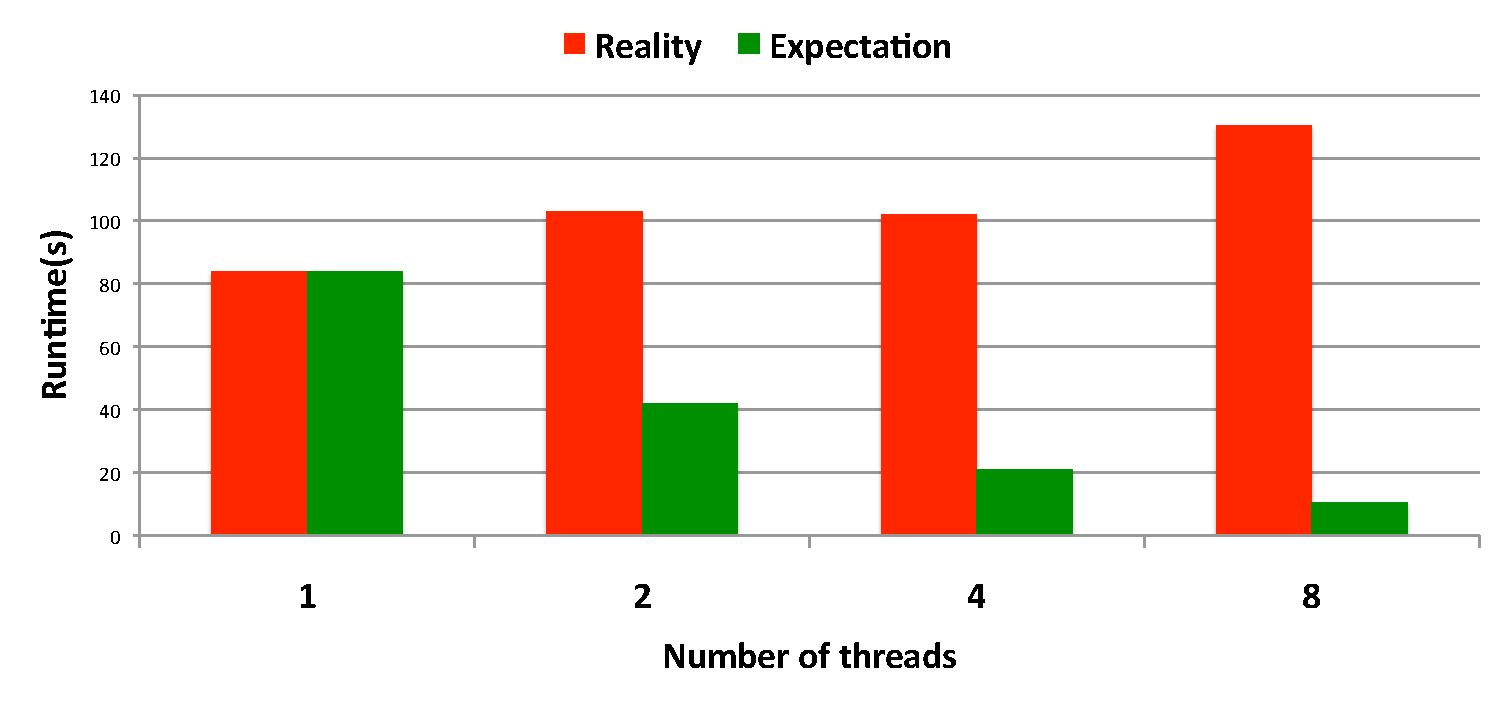
\includegraphics[width=6in]{fig/fsperfimpact.pdf}
\caption{
False sharing performance impact for the simple program shown in Figure~\ref{fig:falsesharingexample}.
\label{fig:fsperfimpact}
}
\end{figure*}

\subsection{Fixing False Sharing}
There are several ways to fix false sharing problems after they are identified. The basic idea is to prevent multiple threads from accessing the same cache line simultaneously.  

The first way is to change the size of corresponding structure or class, by padding some useless words. Thus, we can prevent two threads concurrently accessing the same cache line. One example of prevention, linear\_regression, can be seen in Section~\ref{sec:effecteval}.

The second way is to assign the value to thread-local variables at first. Then different threads only update their own local variables, and commit those changes back to the shared variable in the end. For example, the problem shown in Figure~\ref{fig:falsesharingexample} is fixed using this method, see Figure~\ref{fig:falsesharingexamplefix}. 

\begin{figure*}[!ht]
{\centering
\fbox{
\subfigure{\lstinputlisting[numbers=none,frame=none,boxpos=t]{fig/falsesharing.sample2fix}}
}
\caption{Fixing the false sharing problem shown in Figure~\ref{fig:falsesharingexample}.
\label{fig:falsesharingexamplefix}}
}
\end{figure*}

Some other approaches, to fix false sharing problems automatically, is described in detail in Section~\ref{sec:fspreventwork}, but they all suffer different shortcomings. 






\chapter{Related Work}

\label{chapter:relatedwork}
This chapter first describes those related work to processes-as-threads framework and deterministic execution. Then it describes related work in false sharing detection, prevention, or both. 

\section{Processes-As-Threads framework}

BOP relies on strong isolation of processes to automatically and safely parallelize the execution of programs~\cite{DingBOP}. BOP forks a new process to do speculation, based on those pre-defined possibly parallel regions (PPR). In order to check the correctness, BOP tracks accesses on a page-based granularity. When there is no conflict and a speculative process reaches the end of its current PPR, its predecessor always commits its changes to the current process. However, BOP does not provide any synchronization support and can not be used to run normal multithreaded programs. 

Grace is a process-based approach designed to prevent
concurrency errors, such as deadlock, race conditions, and
atomicity errors by imposing a sequential semantics on
speculatively-executed threads~\cite{grace}. Grace supports only fork-join programs without inter-thread communication (e.g., condition variables or barriers), and rolls back threads when accesses of threads would violate sequential semantics: a thread accesses pages that have been accessed by its predecessors. Grace can not support arbitrary multithreaded programs. Similar to the Grace system, Sammati is a processes-as-threads system to detect and tolerate deadlock problems~\cite{Pyla:2010:ADA:1854273.1854288}. However, Sammati does not support the full range of synchronizations, without synchronizations, barriers, and signals. Also, Semmati can not avoid race conditions happening in creating twin pages, which are avoided by \Sheriff{} framework.

\begin{comment}
% Some usage of this framework
According to Revisions,  Grace cannot easily resolve all
conflicts on commit (like revisions do) and must thus restrict
tasks from producing such conflicts either statically (by type
system) or dynamically (pessimistic with blocking, or optimistic with abort and retry). Also, Grace allows only a restricted “fork-join” form of concurrency
Revisions~\ref{Burckhardt:2010:CPR:1869459.1869515}
\end{comment}

\section{Deterministic Multithreading}
The research on deterministic multithreading is a very active area these years. We describe some software-only, non- language-based approaches here.

\subsection{Software-only deterministic system}
Grace prevents deadlocks, race conditions, ordering and atomicity violations errors for those fork-join multithreaded programs by imposing a sequential semantics at join points~\cite{grace}. However, Grace does not support programs with interthread communications, such as conditional variables and barriers.

CoreDet is a compiler-based approach to 
support general-purpose multithreaded programs~\cite{Bergan:2010:CCR:1736020.1736029}. 
CoreDet instruments those memory read and write operations as long
as those operations can not be proved to be thread-local in static analysis. 
In the runtime phase, CoreDet divides the execution into 
alternating parallel and serial phases and guides all memory operations 
using a memory ownership table: only those owned locations can be accessed
in the parallel phases; all non-owned locations and synchronizations can only 
be accessed in the serial phases guided by a global token.
CoreDet guarantees deterministic execution for racy programs without memory errors,
but with very high performance overhead: 
averagely $3.5\times$ slower than those using \pthreads{} library.
In order to guarantee determinsim, 
CoreDet has to serialize \emph{all} external library calls without instrumentation.
CoreDet doesn not provide deterministic 
memory allocations, which can not guarantee determinism for programs with memory errors.  
% The use of synchronization points as commit boundaries also makes \dthreads{}
% code relatively \emph{robust}: when updates occur after a given number of 
% instructions retired (as in CoreDet and Kendo), it is impossible for 
% programmers to know when interleavings can occur. Such boundaries could vary 
% depending on the underlying architecture and would also be input-dependent, 
% meaning that slightly different inputs could lead to dramatically different
% thread interleavings. By contrast, \dthreads{} guarantees that only changes to
% the sequence of synchronization operations affect the order in which updates 
% are applied.
dOS~\cite{deterministic-process-groups} is an extension to CoreDet
that uses the same deterministic scheduling framework.  dOS 
supports deterministic communication for those threads and processes inside the same
deterministic process groups (DPGs) and handle those external non-determinism by recording and
replaying interactions across DPG boundaries. 

Determinator is a microkernel-based operating system that enforces
system-wide determinism~\cite{efficient-system-enforced}.
Determinator provides separate address spaces and supports interprocess
communications at explicit synchronizaton points. 
Determinator is a proof-of-concept system, which can not support the whole rage of
threads APIs and can not work on legacy programs.  

Some other works can only support limited determinism or need user annotation.
Kendo can only guarantee the determinism for race-free programs~\cite{1508256}. 
TERN~\cite{stable-deterministic} provides a best-effort system to 
apply memoized schedules for future runs with similar inputs. 
It can not guarantee the determinism for racy programs, as Kendo. 
Peregrine~\cite{peregrine:sosp11} is a system based on TERN, which tries to record
 memory accesses orders for racy portion and apply those schedules for future runs possibly.
However, both TERN and Peregrine do not support complete determinism (using a best effort)
and requires program annotations. 

\subsection{Hardware-related deterministic System}

\section{False Sharing}

This section describes related work in false sharing detection, prevention, or both. There is no previous
system to predict unobserved false sharing.

\subsection{False Sharing Detection}
Based on the SIMICS functional simulator, Schindewolf et al.\ designed a tool to report different kinds of cache usage information, such as cache misses and cache invalidations~\cite{falseshare:simulator}. Pluto relies on Valgrind dynamic instrumentation framework to track the sequence of memory read and write events on different threads, and reports a worst-case estimation of possible false sharing~\cite{falseshare:binaryinstrumentation1}.
Similarly, Liu uses Pin to collect memory access information, and reports total cache miss information~\cite{falseshare:binaryinstrumentation2}.
These tools impose about $100-200\times$ performance overhead.

Zhao et al.\ developed a tool based on DynamoRIO framework to detect false sharing and other cache contention problems
for multithreading programs~\cite{qinzhao}. 
It uses a shadow memory technique to maintain memory access history and detects cache invalidations based on the ownership of cache lines. However, it can only support at most $8$ threads. In addition, it cannot differentiate cold cache misses from actual false sharing problems.

Intel's performance tuning utility (PTU) uses Precise Event Based Sampling (PEBS) hardware support to detect false sharing problems ~\cite{detect:ptu, detect:intel}.  PTU cannot distinguish true sharing from false sharing. In addition, PTU aggregates memory accesses without considering memory reuses and access interleaving, leading to numerous false positives. Sanath et al. designed a machine learning based approach to detect false sharing problems. They train their classifier on mini-programs and apply this classifier to general programs ~\cite{mldetect}. Instead of instrumenting memory accesses, this tool relies on hardware performance counters to collect memory accesses events. It achieves very low performance overhead(about 2\%). But it relies on hardware support for its efficiency.  

In addition to their individual disadvantages,
all approaches discussed above share a common shortcoming:  
they cannot pinpoint the exact location of false sharing in the source code, so programmers have to examine the source code and identify problems manually.

Pesterev et al.\ present DProf, a tool that help programmers identify cache misses based on AMD's instruction-based sampling hardware~\cite{DProf}. DProf requires manual annotation to locate data types and object fields, and cannot detect false sharing when multiple objects reside on the same cache line.

\subsection{False Sharing Prevention}
\label{sec:fspreventwork}
% More approaches
Jeremiassen and Eggers use a compiler transformation to automatically adjust the memory layout of applications through padding and alignment~\cite{falseshare:compile}. Chow et al.\ alter parallel loop scheduling in order to avoid false
sharing~\cite{falseshare:schedule}. These approaches only works for regular, array-based scientific code.

Berger et al.\ describe Hoard, a scalable memory allocator that can reduce the possibility of false sharing by making different threads use different heaps~\cite{Hoard}. Hoard cannot avoid false sharing problem in global variables or within
a single heap object: the latter appears to be the primary source of real false sharing problems.

\subsection{False Sharing Detection and Prevention}

Plastic leverages the sub-page granularity memory remapping facility provided by the Xen hypervisor to detect and tolerate false sharing automatically~\cite{OSdetection}. However, the sub-page memory remapping mechanism is not currently supported by most existing operating system, reducing its generality. In addition, Plastic cannot pinpoint the exact source of false sharing.  
In order to utilize Plastic's prevention tool, a program has to run on the Xen hypervisor, limiting the applicability of their prevention technique.



\chapter{\dthreads{}:Efficient Deterministic Multithreading}

\label{sec:introduction}

The advent of multicore architectures has made multithreaded
programming increasingly necessary, but writing multithreaded programs
remains painful. It is notoriously far more challenging to write
concurrent programs than sequential ones because of the wide range of
errors it can cause, including deadlocks and race
conditions~\cite{havender,76897,130623}. Because thread interleavings
are non-deterministic, different runs of the same multithreaded
program can unexpectedly produce different results. These
``Heisenbugs'' greatly complicate debugging, and eliminating them
requires extensive testing to account for possible thread
interleavings~\cite{DBLP:conf/icse/BallBHMQ09,DBLP:conf/asplos/BurckhardtKMN10}.

% Lots of recent work on bug finding. Getting better, but still difficult.

Instead of testing, one promising alternative approach is to attack
the problem of concurrency bugs by eliminating its source:
non-determinism. A fully \emph{deterministic multithreaded system}
would prevent Heisenbugs by ensuring that executions of the same
program with the same inputs always yield the same results, even in
the face of race conditions in the code. Such a system would not only
dramatically simplify debugging of concurrent
programs~\cite{Carver:1991:RTC:624586.625040} and reduce their
attendant testing overhead, but would also enable a number of other
applications. For example, a deterministic multithreaded system would
greatly simplify record and replay for multithreaded
programs~\cite{Choi:1998:DRJ:281035.281041,LeBlanc:1987:DPP:32387.32396}
and the execution of multiple replicas of multithreaded applications
for fault
tolerance~\cite{deterministic-process-groups,1134000,224058,replicant-hotos}.

Several recent software-only proposals aim at providing
deterministic multithreading, but these all suffer from a variety of
disadvantages. Language-based approaches are effective at removing
determinism but require programmers to write code in specialized
languages, which can be
impractical~\cite{Bocchino:2009:TES:1640089.1640097,Burckhardt:2010:CPR:1869459.1869515,Simpson:1999:SEE:330346.330357}. Recent
deterministic systems that target legacy programming languages
(especially C/C++) are either incomplete or impractical. Kendo ensures
determinism of synchronization operations with low overhead, but does
not guarantee determinism in the presence of data
races~\cite{1508256}. Grace prevents all concurrency errors but is
limited to fork-join programs, and although it is efficient, it can require
code modifications to avoid large runtime
overheads~\cite{grace}. CoreDet, a compiler and runtime system,
enforces deterministic execution for arbitrary multithreaded C/C++
programs~\cite{Bergan:2010:CCR:1736020.1736029}. However, it exhibits
prohibitively high overhead (running up to $8\times$ slower
than \pthreads{}; see Section~\ref{sec:evaluation}) and generates
thread interleavings at arbitrary points
in the code, complicating program debugging and testing.

\hspace{1em} \\
\noindent
\textbf{Contributions:}
This paper presents \textbf{\dthreads{}}, an efficient deterministic runtime
system for multithreaded C/C++ applications. \dthreads{} guarantees
deterministic execution of multithreaded programs even in the presence
of data races (notwithstanding external sources of non-determinism
like I/O): given the same sequence of inputs, a program
using \dthreads{} always produces the same output. \dthreads{}'
deterministic commit protocol not only eliminates data races but also
prevents lock-based deadlocks.

\dthreads{} is easy to deploy: it works as a direct replacement for
the \pthreads{} library, requiring no code modifications or
recompilation. \dthreads{} is also efficient. \dthreads{} leverages
process isolation and virtual memory protection to track and isolate
concurrent memory updates, which it deterministically commits. Not
only does this approach greatly reduce overhead versus approaches that
use software read and write barriers, it also eliminates cache-line
based false sharing, a notorious performance problem for multithreaded
programs. These two features combine to enable \dthreads{} to nearly
match or even exceed the performance of \pthreads{} for the majority
of the benchmarks examined here. \dthreads{} thus marks a significant
improvement over the state of the art in deployability and
performance, and provides promising evidence that fully deterministic
multithreaded programming may be practical.

\section{Architecture}

\begin{comment}
Because multithreaded programs frequently use updates to shared memory to communicate, \dthreads{} must implement a mechanism to expose one thread's updates to all other threads.  At the beginning of a transaction, all shared pages are protected, and can only be read by threads.  When a thread attempts to modify a shared page a local working copy is created, leaving the shared page unmodified.  At commit time, a ``twin'' copy of all modified pages is created.  Every page is compared to its twin (using a byte-wise diff) and modified bytes are copied back to the shared state.  Unlike transactional memory, conflicting changes do not result in rollbacks with \dthreads{}.  Further details are described in Section~\ref{sec:sharedmemory}.
\end{comment}


\label{sec:dthreads-architecture}
This section describes \dthreads{}’ key algorithms—memory isolation, deterministic (diff-based) memory commit, deterministic synchronization, and deterministic memory allocation—as well as other implementation details.

\subsection{Isolated Memory Access}
\label{sec:threadsasprocs}

In order to achieve the deterministic memory access, 
\dthreads{} isolates memory accesses among different
threads between commit points, and commits the updates of each thread deterministically. \dthreads{} is based on the \sheriff{} framework, discussed in Section~\ref{sec:sheriffframework}.

Relying on the \sheriff{} framework, \dthreads{} isolates  memory access among different threads: different threads can only see their own local changes. Additionally, \dthreads{} shims the \texttt{getpid()} function to return a single, globally-shared process identifier. 

\subsubsection{Deterministic Thread Index}
\label{sec:threadindex}

POSIX does not guarantee deterministic process or thread identifiers. To avoid exposing this nondeterminism to threads running as processes, \dthreads{} shims the \texttt{pthread\_self()} function in order to return an internal thread index.  This internal thread index is managed using a single global variable that is incremented on thread creation.  This unique thread index is also used to manage per-thread heaps and as an offset into an array of thread entries.

\subsubsection{Shared Memory}
\label{sec:stackandheap}

In order to create the illusion that different threads are sharing the same address space, \dthreads{} uses memory mapped files to share the globals and heap across different processes.

As discussed in Section~\ref{sec:sharedmemory}, \dthreads{} creates two different mappings for both the heap and the globals.  One is a shared mapping, which is used to hold shared state. The other is a private, copy-on-write (COW) per-process mapping that each process works on directly.  Private mappings are linked to the shared mapping through the single fixed-size memory mapped file. Reads initially go directly to the shared mapping,
but after the first write operation, both reads and writes are entirely private.

Memory allocations are issued from the shared heap memory using a scalable per-thread heap organization loosely based on Hoard~\cite{BergerMcKinleyBlumofeWilson:ASPLOS2000} and built using HeapLayers~\cite{BergerZornMcKinley:2001}.  \dthreads{} divides the heap into a fixed number of sub-heaps (currently 16).  Each thread uses a hash of its thread index to find the appropriate sub-heap.

\subsection{Deterministic Memory Commit}
\label{sec:sharedmem}

\begin{figure}
{\centering 
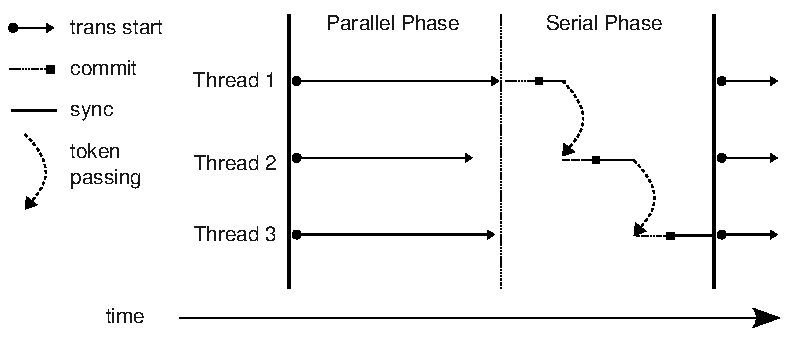
\includegraphics[width=3.25in]{dthreads/figure/phase}
\caption{An overview of \dthreads{} phase. Program execution with \dthreads{} alternates between parallel and serial phases.\label{fig:phase}}
}
\end{figure}

Figure~\ref{fig:phase} illustrates the execution of programs under \dthreads{}.  To guarantee determinism, \dthreads{} isolates memory accesses in parallel phases. In parallel phases, memory accesses work on private copies after the first write operation and updates are not shared across threads.  When a synchronization point is reached, updates are exposed in deterministic order.  This section describes the mechanisms used to guarantee deterministic commit order, and the details of commits to shared memory.

\subsubsection{Fence and Token}
\label{sec:schedule}

\dthreads{} places internal fences between the parallel and serial phases. \dthreads{} re-implements the fence because the standard \pthreads{} barrier mechanism does not support dynamic changes of threads number. 

\begin{figure}
\begin{lstlisting} [style=tt]
void waitFence(void) {
  lock();
	
  while(!isArrivalPhase()) { 
    CondWait();
  }

  waiting_threads++;
  if(waiting_threads < alive_threads) {
    while(!isDeparturePhase()) {
      CondWait();
    }
  } 
  else {
    setDeparturePhase();
    CondBroadcast();
  }

  waiting_threads--;
  if (waiting_threads == 0) {
    setArrivalPhase();
    CondBroadcast();
  }

  unlock();
}

\end{lstlisting}
\caption{Pseudocode for the internal fence.\label{fig:internalFence}}
\end{figure}

Figure~\ref{fig:internalFence} shows the pseudocode code for the internal fence. Threads must wait at the fence until all threads from the previous fence have departed. Then those threads are waiting on the fence until all alive threads  have entered into the same fence(lines 8-11). 
The last thread entering the fence initiates the departure phase and wakes up all threads on the fence(lines 14-15). As threads leave the fence, they decrement the waiting thread count.  The last thread to leave sets the fence to the arrival phase and wakes any waiting threads (lines 19-21).

To reduce overhead, whenever the number of running threads is
less than or equal to the number of cores, waiting threads block by spinning rather than by invoking relatively expensive cross-process \pthreads{} mutexes. When the number of threads exceeds the number of cores, \dthreads{} falls back to using \pthreads{} mutexes.

\begin{figure}
\begin{lstlisting} [style=tt]
void waitToken() {
  waitFence();
  while(isNotMyToken()) { yield(); }
}
void putToken() {
  passTokenToNextOfTokenQueue();
}
\end{lstlisting}
\caption{Pseudocode for waitToken and putToken. 
\label{fig:token}}
\end{figure}

Another key mechanism of \dthreads{} is using the token to order memory commits and synchronizations. The token implementation is listed in Figure~\ref{fig:token}. The token is a shared pointer that points to the next runnable thread entry, which guarantees the global order for all operations in serial phases.  

\dthreads{} introduces two subroutines to manage tokens.  The\texttt{waitToken()} function first waits at the internal fence and then waits to acquire the global token
in order to enter serial mode. The \texttt{putToken()} function passes the token to the next waiting thread. 

As shown in Figure~\ref{fig:phase}, it is very important for a thread to wait at the internal fence before a thread enters into serial phases or before a thread leaves serial phases, even for a thread that is guaranteed to have the token next. Memory commits by a thread can affect other threads' behavior. 

\subsubsection{Commit Protocol}
\begin{figure}
{\centering
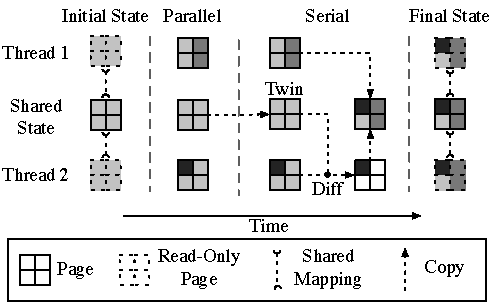
\includegraphics[width=5in]{dthreads/figure/architecture-diagram}
\caption{An overview of \dthreads{} execution.\label{fig:architecture}}
}
\end{figure}

Figure~\ref{fig:architecture} shows the steps to capture modifications to shared state and expose them in a deterministic order.  

At the beginning of the parallel phases, different threads have a read-only mapping for all shared pages. If a thread writes to a shared page during the parallel phases, this write is trapped in order to create a private copy and a twin page for this shared page. After that, reads and writes on this page happen on the private copy only. Reads go directly to the shared memory and are not trapped.  

In the serial phases, threads first commit their local changes happening in parallel phases one at a time, guided by the global token.  The first thread to commit to a page can directly copy its private copy to the shared state, but subsequent commits must copy only the modified bytes. To find out those modifications, \dthreads{} compares those private copies against those twin pages, creating from the shared mapping before actual modification.  After a thread commits its local changes, it issues synchronizations before it passes the token to next thread. 

In the end of serial phase, every threads have to wait at the fence in order to enter into the next parallel phase. 

\subsection{Deterministic Synchronization}
\label{sec:synchronization}
\dthreads{} supports the full range of synchronizations of
\pthreads{} APIs, including locks, conditional variables, barriers and different types of thread exit. Because the \sheriff{} framework can not provide any determinism guarantee, \dthreads{} re-implements all synchronizations as the following.

\subsubsection{Locks}
\dthreads{} uses the global token to guide synchronizations during the serial phases. Before a thread is acquiring a lock while current thread does not have the token, it has to wait for the global token. 

\dthreads{} treats multiple locks as the same one, which  possibly compromise the efficiency of programs, it only ends the serial phases when all locks are unlocked. Thus, it is possible for a program with deadlock problems that those deadlock do not occur to \dthreads{} at all. 

For the acquisitions of locks, \dthreads{} checks at first 
whether the current thread is already holding any locks. If not, the thread first waits for the token, commits those changes happened in the last parallel phase to shared state, and begins a new atomic section. Finally, the thread increments the number of locks it is currently holding. The lock count ensures that a thread does not pass the token to the next one until it has released all of the locks.

During the releases of locks, \dthreads{} decrements the lock count at first. A thread does nothing if there are still some locks holding by the current thread, with the lock count not equal to 0. If all locks have been released, \dthreads{} commits the memory changes happened in this serial phase to the shared mapping. Then it passes the global token to the next thread of the token queue and starts a new atomic region. Finally, the thread waits on the internal fence before entering into the next round's parallel phase.

\subsubsection{Condition Variables}
\label{sec:condwait}

Guaranteeing determinism for condition variables is much more complex than for other synchronization operations. The underlying operating system can not guarantee that threads are going to be waken-up in the same order as they wait on a conditional variable. Thus, a naive implementation easily leads to a deadlock problem.

% pthread_cond_wait: waiting threads are extracted from the 
% the token queue.
% Reducing the performance cost, 
When a thread calls \texttt{pthread\_cond\_wait}, it first acquires the global token and commits local modifications. It then removes itself from the token queue since threads waiting on condition variables do not participate in the token pass of the serial phase until they are awakened. Then, \dthreads{} adds itself to the conditional variable's waiting queue, decreases the alive thread count (used in the internal fence mechanism), and passes the token to the next thread on the token queue before actually waiting on a real process-shared conditional variable. When a thread is awaken, it should check at first whether the current thread is ready to run or not. For threads waken up by \texttt{pthread\_cond\_signal}, only the first thread in the waiting list can run in order to guarantee the First-In-First-Out order. All threads can run if waken up by \texttt{pthread\_cond\_broadcast}. If a thread is not able to run, it waits on the conditional variable again. If a thread is the candidate thread to be waken up, it waits for the global token because a thread waking up from a conditional variable is supposed to acquire the mutex, which means that it should already have the global token. 

For those waken-up functions, including \texttt{pthread\_cond\_signal} and \texttt{pthread\_cond\_broadcast}, the calling thread first waits for the token, and then commits any local modifications. If no threads are waiting on the condition variable, \dthreads{} passes the token to the next thread immediately. Otherwise, \dthreads{} moves corresponding threads in the condition variable queue to the head of the token queue, marked them as ready, and increments the live thread count correspondingly. To guarantee that threads are waken-up in the same order as they wait on a conditional variable, \texttt{pthread\_cond\_signal} only do this for the first thread in the queue but \dthreads{} wakes up all threads simultaneously. Those not-ready threads immediately wait again after waken-up. In order to improve the performance, those newly waken-up threads are scheduled to run next by simply putting them into the header of the token queue so that the calling thread can pass the token to them. 


\subsubsection{Barriers}

\label{sec:barrierwait}

\dthreads{} must ensure that threads waiting on a barrier do not disrupt the token passing of running threads. \dthreads{} removes threads entering into the barrier from the run queue and places them on the corresponding barrier queue.

In order to ensure the deterministic commit, the calling thread first waits for the global token to commit any local modifications. If the current thread is the last one to enter the barrier, \dthreads{} moves all threads on the barrier queue to the token queue, increases the alive threads count, and passes the token to the first thread in the barrier queue.  Otherwise, \dthreads{} removes the current thread from the token queue, places it on the barrier queue, releases the token. and waits on the actual barrier.


\subsubsection{Thread Creation and Exit}

\label{sec:threadcreation}

\begin{figure}
\begin{lstlisting} [style=tt]
void thread_create () {
  waitToken();
  clone(CLONE_FS| CLONE_FILES | CLONE_CHILD);
  if(isChild) {
    allocGlobalThreadIndex();
    insertToTokenQueue();
	notifyChildRegistered();
	// Wait for the parent to reach next sync point
    waitParentBroadcast();	
  }
  else if (isParent) {
    waitChildRegistered();
  }
}
\end{lstlisting}
\begin{lstlisting} [style=tt]
void thread_exit() {
  waitToken();
  atomicEnd(false);
  removeFromTokenQueue();
  decreaseInternalFence();
  putToken();
  exitThread(); 
}
\end{lstlisting}
\caption{Pseudocode for thread creation and exit($\S$~\ref{sec:threadcreation}).
\label{fig:threadcreation}
}
\end{figure}

To guarantee determinism, thread creation and exit must be performed in the serial phases.  Newly created threads are immediately added to the token queue.  For performance reason, the spawning thread does not immediately release the token until next different synchronization. This allows a single thread to quickly create multiple child threads without waiting for a new serial phase.

Figure~\ref{fig:threadcreation} shows pseudocode for thread creation and thread exit. The calling thread firstly waits for the token before proceeding (line 2).  It then creates a new process with shared file descriptors but a distinct address space using the \texttt{clone} system call (line 3).  The newly created child obtains the global thread index (line 5), places itself in the token queue (line 6), and notifies the parent that child has registered itself in the token queue(line 7). The child thread then waits for the parent to reach the next synchronization point. 

When \texttt{thread\_exit()} is called, the caller first waits for the token and then commits any local modifications (line 3). It then removes itself from the token queue (line 4) and decreases the number of threads required to proceed to the next phase (line 5). Finally, the thread passes its token to the next thread in the token queue (line 6) and exits (line 7).

\subsubsection{Thread Cancellation}

\dthreads{} implements the thread cancellation in serial phases in order to guarantee the determinism. phase. A thread can only invoke \texttt{pthread\_cancel} while holding the token. If the thread being cancelled is waiting on a condition variable or a barrier, it is removed from the queue deterministically. Finally, to cancel the corresponding thread, \dthreads{} kills the target process using kill(tid, SIGKILL) and the number of alive threads should be decremented after the cancellation.

\subsection{Deterministic Memory Allocation}
Programs sometimes rely on the addresses of objects returned by the memory allocator intentionally (for example, by hashing objects based on their addresses), or accidentally. A program with a memory error, like a buffer overflow, will yield different results for different memory layouts.

This reliance on memory addresses can undermine other efforts to provide determinism. For example, CoreDet is unable to fully enforce determinism because it relies on the Hoard scalable memory allocator~\cite{Bergan:2010:CCR:1736020.1736029}. Hoard was not designed to provide determinism and several of its mechanisms, thread id based hashing and non-deterministic assignment of memory to threads, lead to nondeterministic execution in CoreDet for the canneal benchmark.


To preserve determinism in the face of intentional or inadvertent reliance on memory addresses, we designed the \dthreads{} memory allocator to be fully deterministic. \dthreads{} assigns subheaps to each thread based on its thread index (deterministically assigned; see Section 4.1.2). In addition to guaranteeing the same mapping of threads to subheaps on repeated executions, \dthreads{} allocates superblocks (large chunks of memory) deterministically
by acquiring a lock (and the global token) on each
superblock allocation. Thus, threads always use the same subheaps, and these subheaps always contain the same superblocks on each execution. The remainder of the memory allocator is entirely deterministic. The superblocks themselves are allocated via mmap: while \dthreads{} could use a fixed address mapping for the heap, we currently simply disable ASLR to provide deterministic mmap calls. If a program does not use the absolute address of any heap object, \dthreads{} can guarantee determinism even with ASLR enabled.
Hash functions and lock-free algorithms frequently use absolute addresses, and any deterministic multithreading system must disable ASLR to provide deterministic results for these cases.


\section{Optimizations}
\label{sec:dthreads-optimization}

\dthreads{} performs a number of optimizations to improve performance.

\textbf{Lazy commit:} \dthreads{} reduces copying overhead and the time spent in the serial phase by lazily committing pages. When only one thread has ever modified a page, \dthreads{} considers that thread to be the page’s owner. An owned page is committed to shared state only when another thread attempts to read or write this page, or when the owner thread attempts to modify it in a later phase. \dthreads{} tracks reads with page protection and signals the owning thread to commit pages on demand. To reduce the number of read faults, pages holding global variables (which we expect to be shared) and any pages in the heap that have ever had multiple writers are all considered unowned and are not read-protected.

\textbf{Single-threaded-execution: }
When only one thread is running, \dthreads{} does not employ memory protection and treats all synchronization operations as no-ops. In addition, when only one thread is active because other threads are waiting on conditional variables, 
\dthreads{} does not try to commit local changes to the shared mapping (or discard private dirty pages). Updates are only committed when the thread issues a \texttt{cond\_signal} or \texttt{cond\_broadcast} call, which will wake up a thread and thus require publication of any updates.

\textbf{Lazy twin creation and diff elimination: }
Twin pages are only created when a page has multiple writers during the same phase. Also, \dthreads{} can commit its local changes by directly copying its working copy to the shared state, without performing a diff. This reduces the cost of a twin page allocation, a page copy, and a diff operation when a single thread is the exclusive writer of a page.

\textbf{Lock ownership:} \dthreads{} uses lock ownership to avoid unnecessary waiting when threads are using distinct locks. Initially, all locks are unowned. Any thread that attempts to acquire a lock that it does not own must wait until the serial phase to do so. If multiple threads attempt to acquire the same lock, this lock is marked as shared. If only one thread attempts to acquire the lock, this thread takes ownership of the lock and can acquire and release
it during the parallel phase. Lock ownership can result in starvation if one thread continues to re-acquire an owned lock without entering the serial phase. To avoid this, each lock has a maximum number of times it can be acquired during a parallel phase before a serial phase is required.

\textbf{Parallelization: }
\dthreads{} attempts to exploit as much parallelism as possible in the runtime system itself. One optimization is that at the start of transactions, \dthreads{} performs certain cleanup tasks, including releasing private page frames or resetting pages to read-only mode. It is safe to perform these cleanup tasks since these operations do not affect other the behavior of other threads.
Thus, \dthreads{} parallelizes a thread's cleanup tasks with other threads’ commit operations, without holding the global token. With this optimization, the token is passed to the next thread as soon as possible, saving time in the serial phase. 

\section{Implementation}
aaa


\section{Evaluation}
\label{sec:dthreadsevaluation}

We perform our evaluation on an Intel Core 2 dual-processor CPU system, equipping with 16GB of RAM. Each processor is a 4-core 64-bit Xeon, running on at 2.33GHZ with a 4MB L2 cache. The operating system is an unmodified CentOS 5.5, running with Linux kernel version 2.6.18-194.17.1.el5.

\subsection{Methodology}

We evaluate the performance and scalability of \dthreads{} versus CoreDet and \pthreads{} across the PARSEC~\cite{parsec} and Phoenix~\cite{phoenix-hpca} benchmark suites.  

In order to compare performance directly against CoreDet, which relies on the LLVM infrastructure~\cite{LLVM:CGO04}, all benchmarks are compiled with the LLVM compiler at the ``-O5'' optimization level~\cite{LLVM:CGO04}. Since \dthreads{} does not currently support 64-bit binaries, all benchmarks are compiled for 32 bit environments (using the ``-m32'' compiler flag). Each benchmark is executed ten times on a quiescent machine. To reduce the effect of outliers, the lowest and highest execution times for each benchmark are discarded,
so each result represents the average of the remaining eight runs.

\textbf{Tuning CoreDet:} 
The performance of CoreDet~\cite{Bergan:2010:CCR:1736020.1736029} is extremely sensitive to three parameters: the granularity for the ownership table (in bytes), the quantum size (in number of instructions retired), and the choice between full serial mode and reduced serial mode. We compare the performance and scalability of \dthreads{} with the best possible results that we could obtain for CoreDet on our system---that is, with the lowest average normalized
runtimes---after an extensive search of the parameter space (six possible granularities and 8 possible quanta, for each benchmark). The results presented here are for a 64-byte granularity, a quantum size of 100,000 instructions, and in full serial mode.

\textbf{Unsupported Benchmarks}: We do not include results for 7 benchmarks from PARSEC, since they do not currently work with \dthreads{} (note that many of these also do not work for CoreDet). \texttt{vips} and \texttt{raytrace} would not build as 32-bit executables; \texttt{bodytrack}, \texttt{facesim}, and \texttt{x264} depend on sharing of stack variables;
\texttt{fluidanimate} uses ad-hoc synchronization, so it will not run without modifications; and \texttt{freqmine} does not use \pthreads{}.

 
\textbf{Scalability Experiment}: For all scalability experiments, we logically disable CPUs using Linux's CPU hotplug mechanism, which allows us to disable or enable individual CPUs by writing ``0'' (or ``1'') to a special file (\texttt{/sys/devices/system/cpu/cpuN/online}).

\subsection{Determinism}

We first experimentally verify \dthreads{}' ability to ensure determinism by executing the \emph{racey} determinism tester~\cite{1508256}. This stress test contains, as its name suggests, numerous data races and is thus extremely sensitive to memory-level non-determinism. \dthreads{} reports the same results for 2,000 runs. We also compared the schedules and outputs of all benchmarks used to ensure that every execution is identical.

\subsection{Performance}
\label{sec:performance}

\begin{figure*}[!t]
{\centering
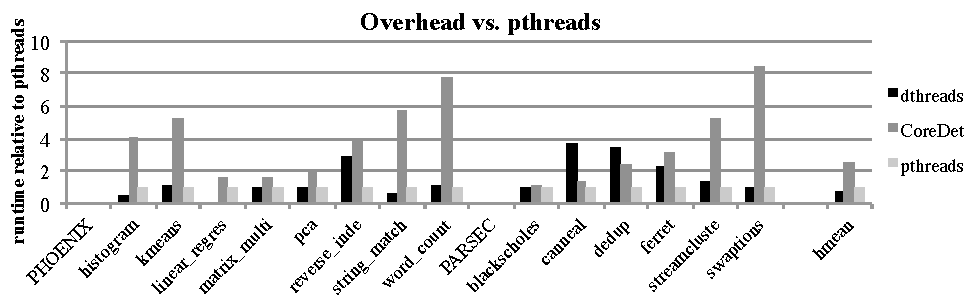
\includegraphics[width=6in]{dthreads/figure/overhead-figure}
\caption{Normalized execution time with respect to \pthreads{} and CoreDet(lower is better). For 9 of the 14 benchmarks, \dthreads{} runs nearly as fast or faster than \pthreads{}, while providing deterministic behavior.\label{fig:performance}}
}
\end{figure*}

\begin{table*}[!t]
\centering
\resizebox{\columnwidth}{!}{
\begin{tabular}{l|rrr|rr|l}
{\bf \small Benchmark} & {\bf \small CoreDet} & {\bf \small \dthreads{}} & {\bf \small \pthreads{}} & $\frac{\mbox{\bf \small CoreDet}}{\mbox{\bf \small \pthreads{}}}$ & $\frac{\mbox{\small \bf \dthreads{}}}{\mbox{\small \bf \pthreads{}}}$ & {\bf \small Input} \\

\hline
{\bf \small histogram} & 0.97 & 0.73 & 0.35 & $1.32\times$ & $0.48\times$ & {\it \small large.bmp} \\
{\bf \small kmeans} & 68.41 & 13.16 & 15.02 & $5.20\times$ & $1.14\times$ & {\it \small -d 3 -c 1000 -p 100000 -s 1000} \\ 
{\bf \small linear\_regression} & 6.42 & 4.11 & 0.57  & $1.56\times$ & $0.14\times$ & {\it \small key\_file\_500MB.txt} \\
{\bf \small matrix\_multiply} & 31.68 & 19.32 & 19.28  & $1.63\times$ & $0.99\times$ & {\it \small 2000 2000 } \\
{\bf \small pca} & 39.24 & 20.49 & 21.14  & $1.92\times$ & $1.03\times$ & {\it \small -r 4000 -c 4000 -s 100 } \\
{\bf \small reverse\_index} & 7.85 & 2.06 & 6.53 & $3.81\times$ & $3.17\times$ & {\it \small datafiles} \\
{\bf \small string\_match} & 18.31 & 3.19 & 1.97 & $5.74\times$ & $0.62\times$ & {\it \small key\_file\_500MB.txt} \\
{\bf \small word\_count} & 17.17 & 2.17 & 2.37 & $7.91\times$ & $1.09\times$ & {\it \small word\_100MB.txt} \\
{\bf \small blackscholes} & 10.49 & 9.47 & 9.30 & $1.11\times$ & $0.98\times$ & {\it \small 8 in\_1M.txt prices.txt} \\
{\bf \small canneal} & 14.74 & 10.41 & 39.82 & $1.42\times$ & $3.83\times$ &  {\it \small 7 15000 2000 400000.nets 128} \\
{\bf \small dedup} & 3.38 & 1.45 & 5.39 & $2.33\times$ & $3.72\times$ & {\it \small -c -p -f -t 2 -i media.dat output.txt} \\
{\bf \small ferret} & 21.89 & 7.02 & 26.86 & $3.11\times$ & $3.83\times$ & {\it \small corel lsh queries 10 20 1 output.txt} \\
{\bf \small streamcluster} & 14.33 & 2.74 & 4.61 & $5.23\times$ & $1.68\times$ &  {\it \small 10 20 128 16384 16384 1000 none output.txt 8} \\
{\bf \small swaptions} & 35.21 & 4.18 & 3.88 & $8.42\times$ & $0.93\times$ & {\it \small -ns 128 -sm 50000 -nt 8} \\
\hline
\end{tabular}
}
\caption{Benchmarks: execution time (in seconds) and input parameters.\label{tbl:benchmarks}}
\end{table*}

We next compare the performance of \dthreads{} to CoreDet
and \pthreads{}. Figure~\ref{fig:performance} presents these results graphically (normalized to \pthreads{}); Table~\ref{tbl:benchmarks} provides detailed information about execution time and input parameters.

\dthreads{} outperforms CoreDet on 12 out of 14 benchmarks (running between 20\% and $11.2\times$ faster). For 9 benchmarks, \dthreads{} runs nearly the same as or better
performance than \texttt{pthreads}. Because \dthreads{} isolates updates in separate processes, it can improve performance by eliminating false sharing: since concurrent ``threads'' actually execute in different physical pages, there is no coherence traffic caused by false sharing between synchronization points. \dthreads{} eliminates catastrophic false sharing in the \texttt{linear\_regression} benchmark, allowing it to execute over $7\times$ faster than \pthreads{} and $11\times$ faster than CoreDet. The \texttt{string\_match} benchmark exhibits a similar, though less dramatic, false sharing problem, allowing \dthreads{} to run almost 60\% faster than \pthreads{} and $9\times$ faster than CoreDet. Two benchmarks, \texttt{histogram} and \texttt{swaptions}, also run faster with \dthreads{} than with \pthreads{} ($2\times$ and $6\%$, respectively; $2.7\times$ and $9\times$ faster than with CoreDet). We believe but have not yet verified that the reason is false sharing.

For some benchmarks, \dthreads{} incurs modest overhead. For example, unlike most benchmarks examined here, which create long-lived threads, the \texttt{kmeans} benchmark creates and destroys over 1,000 threads in the course of its execution. 
While Linux processes are relatively lightweight, creating and exiting a process is still more expensive than the same operations of threads, accounting for a 14\% performance degradation of \dthreads{} over \pthreads{} (though it runs $4.6\times$ faster than CoreDet).

\dthreads{} runs substantially slower than \pthreads{} for 4 of the 14 benchmarks examined here. The \texttt{ferret} benchmark relies on an external library to analyze image files during the first stage in its pipelined execution model; this library makes intensive (and in the case of \dthreads{}, unnecessary) use of locks. Lock acquisition and release in \dthreads{} imposes higher overhead than ordinary \pthreads{} mutex operations. More importantly in this case, the intensive use of locks in one stage forces \dthreads{} to effectively serialize the other stages in the pipeline, which must repeatedly wait on these locks to enforce a deterministic lock acquisition order. The other three benchmarks (\texttt{canneal}, \texttt{dedup}, and \texttt{reverse\_index}) modify a large number of pages. With \dthreads{}, each page modification triggers a segmentation violation, a system call to change memory protection, the creation of a private copy of the page, and a subsequent copy into the shared space on commit (see Section~\ref{sec:future-work} for planned optimizations that may reduce this cost). We note that CoreDet also substantially degrades performance for these benchmarks, so much of this slowdown may be inherent to any deterministic runtime system.

\subsection{Scalability}
\label{sec:scalability}

\begin{figure}
{\centering
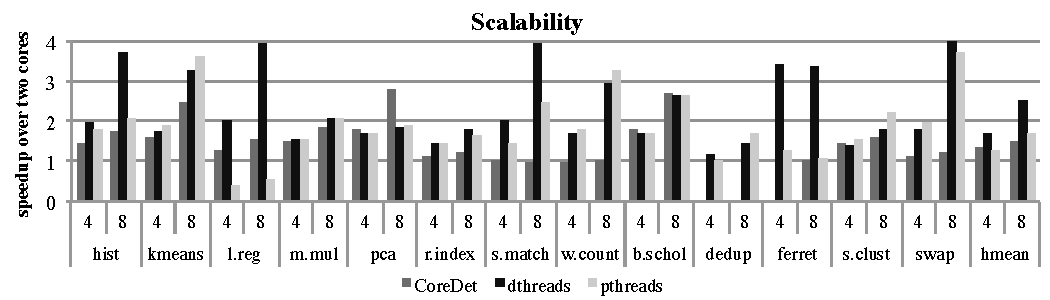
\includegraphics[width=6in]{dthreads/figure/scalability-figure}
\caption{Speedup of eight cores versus two cores (higher is better).  When possible to control with command line options, the number of threads was matched to the number of cores enabled.\label{fig:scalability}}
}
\end{figure}

To measure the scalability cost of running \dthreads{}, we ran two benchmark suite (excluding \texttt{canneal}) on the same machine with eight cores and again with two cores enabled.  Whenever possible without source code modifications, the number of threads was matched to the number of CPUs enabled.  We have found that \dthreads{} scales at least as well as \pthreads{} for 9 of 13 benchmarks, and scales as well or better than CoreDet for all but one benchmark where \dthreads{} outperforms CoreDet by 2x.  Detailed results of this experiment are presented in Figure~\ref{fig:scalability} and discussed below.

\texttt{canneal} was excluded from the scalability experiment because this benchmark does more work when more threads are present, making the performance comparison between eight and two threads unfair.  \dthreads{} hurts scalability relative to \pthreads{} for four of the benchmarks: \texttt{kmeans}, \texttt{word\_count}, \texttt{dedup}, and \texttt{streamcluster} although only marginally in most cases.  In all of these cases, \dthreads{} scales better than CoreDet.

\dthreads{} is able to match the scalability of \pthreads{} for three benchmarks: \texttt{matrix\_multiply}, \texttt{pca}, and \texttt{blackscholes}.  With \dthreads{}, scalability actually \emph{improves} over \pthreads{} for 6 out of 13 benchmarks: \texttt{histogram}, \texttt{linear\_regression}, \texttt{reverse\_index}, \texttt{string\_match}, \texttt{ferret}, and \texttt{swaptions}.




\subsection{Performance Analysis}

\subsubsection{Benchmark Characteristics}

The data presented in Table~\ref{tbl:characteristics} are obtained from the executions running on all 8 cores.  Column 2 shows the percentage of time spent in the serial phases.  In \dthreads{}, all memory commits and actual synchronization operations are performed in the serial phases.  The percentage of time spent in the serial phases thus can affect performance and scalability. Applications with higher overhead in \dthreads{} often spend a higher percentage of time in the
serial phases, primarily because they modify a large number of pages that need to be committed during those phases.

Column 3 shows the number of transactions in each application and Column 4 provides the average length of each transaction (ms).  Every synchronization, including locks, conditional variable, barriers, and thread exits, demarcate transaction boundaries in \dthreads{}.  For example, \texttt{reverse\_index}, \texttt{dedup}, \texttt{ferret}
and \texttt{streamcluster} perform numerous transactions whose
execution time is less than 1ms, imposing a performance penalty for these applications.  Benchmarks with longer (or fewer) transactions run almost the same speed as or faster than \texttt{pthreads}, including \texttt{histogram} or \texttt{pca}.  In \dthreads{}, longer transactions amortize the overhead of memory protection and copying.

Column 5 and 6 provides more detail on the costs associated with memory updates (the number and total volume of dirtied pages). From the table, it is clear why \texttt{canneal} (the most notable outlier) runs much slower with \dthreads{} than with \pthreads{}. This benchmark updates over three million pages, leading to large performance overhead caused by creating  private copies, handling protection faults, and committing modifications on those pages to the shared memory space. 

\textbf{Conclusion: }
Most benchmarks examined here contain either a small number of transactions, thus having long running transactions, and modify a modest number of pages during execution. For these applications, \dthreads{} is able to amortize its overhead: by eliminating false sharing, it can even run faster than \pthreads{}. However, for the few benchmarks that perform numerous short-lived transactions, or modify a large amount of pages, \dthreads{} can introduce substantial overhead.


\begin{table*}[!t]
\centering
\resizebox{\columnwidth}{!}{
\begin{tabular}{l|rrrrr}
& {\bf \small Serial Phase} & {\bf \small Transactions} & {\bf \small TransLength} & {\bf \small DirtyPages} & {\bf \small DirtyPages}
\\
{\bf \small Benchmark} & {\bf \small (\% of time)} & {\bf (\#)} & {\bf \small (ms)} & {\bf \small (\#)} & {\bf \small (GB)}\\
%\hline
%\multicolumn{6}{|c|}{\emph{Phoenix}} \\
\hline
\small \textbf{histogram} & 0 & 23 & 15.47 & 29 & 0 \\
\small \textbf{kmeans} & 0 & 3929 & 3.82 & 9466 & 0.04\\
\small \textbf{linear\_regression} & 0 & 24 & 23.92 & 17 & 0\\
\small \textbf{matrix\_multiply} & 0 & 24 & 841.2 & 3945 & 0.02\\
\small \textbf{pca} & 0 & 48 & 443 & 11471 & 0.04 \\
\small \textbf{reverseindex} & 17\% & 61009 & 1.04 & 451876 & 1.72\\
\small \textbf{string\_match} & 0 & 24 & 82 & 41 & 0 \\
\small \textbf{word\_count} & 1\% & 90 & 26.5 & 5261 & 0.02\\
%\hline
%\multicolumn{6}{|c|}{\emph{PARSEC}} \\
%\hline
\small \textbf{blackscholes} & 0 & 24 & 386.9 & 991 & 0\\
\small \textbf{canneal} & 26.4\% & 1062 & 43 & 3606413 & 13.75\\
\small \textbf{dedup} & 31\% & 45689 & 0.1 & 356589 & 1.36\\
\small \textbf{ferret} & 12.3\% & 484127 & 0.05 & 844184 & 3.21 \\
\small \textbf{streamcluster} & 18.4\% & 130001 & 0.04 & 131992 & 0.50\\
\small \textbf{swaptions} & 0 & 24 & 163 & 867 & 0\\
\hline
\end{tabular}
}
\caption{Benchmark characteristics.\label{tbl:characteristics}}
\end{table*}

\subsubsection{Performance Impact Analysis}
We further evaluate the performance impact of two important components of \dthreads: deterministic synchronization (sync-only) and memory protection(prot-only).

\emph{Sync-only}: This configuration enforces a deterministic synchronization order. However, the memory protection is not enabled so different processes access the shared memory directly. We want to use this to show the performance impact of load imbalance, caused by synchronization based scheduling.

\emph{Prot-only}: This configuration runs threads in isolation, with commits at synchronization points. The order of synchronization and memory commits are non-deterministic. This configuration eliminates false sharing, but also introduces the performance overhead of isolation and memory commits. In order to guarantee correct execution, we replaced those synchronizations as corresponding cross-processes synchronizations. The lazy twin creation and single-threaded execution optimizations are disabled here because they are unsafe without deterministic synchronization. Thus, this configuration actually evaluates the performance of using the \sheriff{} framework. 


\begin{figure*}[!t]
{\centering
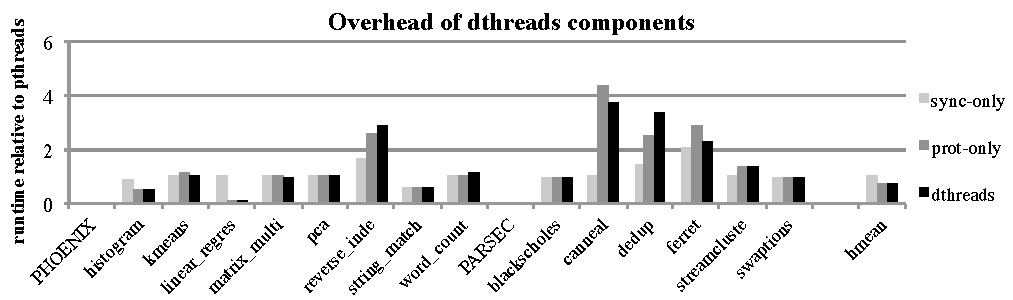
\includegraphics[width=6in]{dthreads/figure/perfeffect}
\caption{Normalized execution time with respect to \pthreads{} (lower is better) for three different configurations. 
\label{fig:perfanalysis}}
}
\end{figure*}

The performance results of these two configurations are shown in Figure~\ref{fig:perfanalysis} and discussed in the following.

\begin{itemize}

\item
The \texttt{reverse\_index}, \texttt{dedup} and \texttt{ferret} benchmarks show significant load imbalance under {\it sync-only} configuration. Additionally, these benchmarks introduces significant overhead with {\it prot-only} configuration because of a large number of transactions there. That explains why \dthreads{} doesn't have good performance on these benchmarks.

\item
The \texttt{string\_match} benchmark shows performance improvement with {\it sync-only} configuration. The exact reason is not clear, may be due to the per-thread allocator. 

\item
The \texttt{linear\_regression}, \texttt{histogram} and \texttt{swaptions} benchmarks improve performance with {\it prot-only} configuration. The memory isolation mechanism eliminates the false sharing problem inside and contributes to the performance speedup.

\item
Normally the performance of \dthreads{} is not better than the performance of {\it prot-only} configuration. However, both \texttt{ferret} and \texttt{canneal} run faster with determinism enabled. Both are benefited from specific optimization described in Section~\ref{sec:dthreads-optimization}. \texttt{ferret} benefits from the \emph{single-threaded-execution}. The performance improvement of \texttt{canneal} is coming from shared twin pages for all threads in the phase.

\end{itemize}








\chapter{\DoubleTake{}: Evidence-Based Dynamic Analysis}
%DIF PREAMBLE EXTENSION ADDED BY LATEXDIFF
%DIF UNDERLINE PREAMBLE %DIF PREAMBLE
\RequirePackage[normalem]{ulem} %DIF PREAMBLE
\RequirePackage{color}\definecolor{RED}{rgb}{1,0,0}\definecolor{BLUE}{rgb}{0,0,1} %DIF PREAMBLE
\providecommand{\DIFadd}[1]{{\protect\color{blue}\uwave{#1}}} %DIF PREAMBLE
\providecommand{\DIFdel}[1]{{\protect\color{red}\sout{#1}}}                      %DIF PREAMBLE
%DIF SAFE PREAMBLE %DIF PREAMBLE
\providecommand{\DIFaddbegin}{} %DIF PREAMBLE
\providecommand{\DIFaddend}{} %DIF PREAMBLE
\providecommand{\DIFdelbegin}{} %DIF PREAMBLE
\providecommand{\DIFdelend}{} %DIF PREAMBLE
%DIF FLOATSAFE PREAMBLE %DIF PREAMBLE
\providecommand{\DIFaddFL}[1]{\DIFadd{#1}} %DIF PREAMBLE
\providecommand{\DIFdelFL}[1]{\DIFdel{#1}} %DIF PREAMBLE
\providecommand{\DIFaddbeginFL}{} %DIF PREAMBLE
\providecommand{\DIFaddendFL}{} %DIF PREAMBLE
\providecommand{\DIFdelbeginFL}{} %DIF PREAMBLE
\providecommand{\DIFdelendFL}{} %DIF PREAMBLE
%DIF END PREAMBLE EXTENSION ADDED BY LATEXDIFF

%\documentclass{sigplanconf}
%\nocaptionrule

% \documentclass[twocolumn,9pt]{article}
% \documentclass[twocolumn,10pt]{acm_proc_article-sp}

% \documentclass{acm_proc_article-sp}
\documentclass[9pt]{sigplanconf}

\date{} % \vspace*{-0.2in}}

% Make sure to put back 

\newcommand{\punt}[1]{}

\punt{

Notes from Daan Leijen:
}

\usepackage{endnotes,xspace}

\newcommand{\footnotenonumber}[1]{{\def\thempfn{}\footnotetext{\small #1}}}
\usepackage[normalem]{ulem}
\usepackage{graphicx}

\usepackage{mathptmx} % rm & math
\usepackage[scaled=0.90]{helvet} % ss
\usepackage{courier} % tt
% \normalfont
\usepackage[T1]{fontenc}

% \usepackage{lmodern}
% \usepackage{times}
\usepackage{subfigure}
\usepackage{url}
\urlstyle{rm}
\usepackage[
      colorlinks=false,    %no frame around URL
      urlcolor=black,    %no colors
      menucolor=black,    %no colors
      linkcolor=black,    %no colors
      pagecolor=black,    %no colors
]{hyperref}

\usepackage{color}
\usepackage{listings}
\usepackage{amsmath}
\usepackage{amsfonts}
\usepackage{amssymb}
\usepackage{comment} 
\usepackage{setspace}
\singlespacing
%\onehalfspacing
\newtheorem{thm}{Theorem}
\newtheorem{prop}[thm]{Proposition}
\newtheorem{cor}[thm]{Corollary}
\newtheorem{lem}[thm]{Lemma}
\newtheorem{defn}[thm]{Definition}

\newcommand{\cfunction}[1]{{\bf \tt #1}}
\newcommand{\malloc}{\cfunction{malloc}}
\newcommand{\realloc}{\cfunction{realloc}}
\newcommand{\free}{\cfunction{free}}
\newcommand{\madvise}{\cfunction{madvise}}
\newcommand{\brk}{\cfunction{brk}}
\newcommand{\sbrk}{\cfunction{sbrk}}
\newcommand{\mmap}{\cfunction{mmap}}
\newcommand{\munmap}{\cfunction{munmap}}
\newcommand{\mprotect}{\cfunction{mprotect}}
\newcommand{\mlock}{\cfunction{mlock}}

\hyphenation{app-li-ca-tion}
\hyphenation{Die-Hard}
\hyphenation{Ar-chi-pe-la-go}
\hyphenation{buf-fer}
\hyphenation{D-threads}
\hyphenation{Heap-Layers}
\hyphenation{wait-Token}
\hyphenation{mul-ti-threa-ded}
\hyphenation{me-m-ory}

\hyphenation{pthread-create}
\hyphenation{pthread-self}
\hyphenation{pthread-mutex-lock}
\hyphenation{pthread-mutex-unlock}

\newcommand{\dthreads}{{\scshape Dthreads}}
\newcommand{\Dthreads}{{\scshape Dthreads}}
\newcommand{\doubletake}{{\scshape DoubleTake}}
\newcommand{\DoubleTake}{{\scshape DoubleTake}}
\newcommand{\stopgap}{{\scshape DoubleTake}}
\newcommand{\Stopgap}{{\scshape DoubleTake}}
\newcommand{\StopGap}{{\scshape DoubleTake}}
\newcommand{\Sheriff}{{\scshape Sheriff}}
\newcommand{\sheriff}{{\scshape Sheriff}}
\newcommand{\Grace}{{\scshape Grace}}
\newcommand{\grace}{{\scshape Grace}}
\newcommand{\SheriffProtect}{\textsc{Sheriff-Protect}}
\newcommand{\sheriffProtect}{\textsc{Sheriff-Protect}}
\newcommand{\sheriffprotect}{\textsc{Sheriff-Protect}}
\newcommand{\SheriffDetect}{\textsc{Sheriff-Detect}}
\newcommand{\sheriffDetect}{\textsc{Sheriff-Detect}}
\newcommand{\sheriffdetect}{\textsc{Sheriff-Detect}}
\newcommand{\pthreads}{\texttt{pthreads}}

\definecolor{lightgray}{rgb}{.9,.9,.9}
\definecolor{darkgray}{rgb}{.4,.4,.4}
\definecolor{purple}{rgb}{0.65, 0.12, 0.82}

\lstdefinelanguage{c++threads}[]{c++}{
  morekeywords={pthread_create,pthread_join},
  keywordstyle=\color{blue}\bfseries,
  ndkeywords={class, export, boolean, throw, implements, import, this},
  ndkeywordstyle=\color{darkgray}\bfseries,
  identifierstyle=\color{black},
  sensitive=false,
  comment=[l]{//},
  morecomment=[s]{/*}{*/},
  commentstyle=\color{purple}\ttfamily,
  stringstyle=\color{red}\ttfamily,
  morestring=[b]',
  morestring=[b]"
}
\lstset{
   language=c++threads,
   backgroundcolor=\color{lightgray},
   extendedchars=true,
   basicstyle=\footnotesize\ttfamily,
   showstringspaces=false,
   showspaces=false,
   numbers=none,
   numberstyle=\footnotesize,
   numbersep=9pt,
   tabsize=2,
   breaklines=true,
   showtabs=false,
   captionpos=b
}
%\lstset{language=c++threads, basicstyle=\ttfamily\scriptsize,frame=trbl,tabsize=4} % ,numbers=left,numberstyle=\tiny}

\definecolor{Gray}{cmyk}{0,0,0,0.5}

\begin{document}

\CopyrightYear{2014}
\copyrightdata{XXX-X-XXXXX-XXX-X/XX/XX}

\title{{\huge \bf \doubletake{}}: Evidence-Based Dynamic Analysis}
% Efficiently and Precisely Locating Buffer Overflows}

% \authorinfo{\emph{authorship list removed for anonymity}}

%\punt{
\authorinfo{Tongping~Liu \and Charlie~Curtsinger \and Emery~D.~Berger}
{School of Computer Science \\
University of Massachusetts Amherst \\
Amherst, MA 01003 \\
{\{tonyliu,charlie,emery\}@cs.umass.edu}
}

\punt{
\numberofauthors{1}
\author{
\alignauthor Tongping~Liu and Emery~D.~Berger \\
\affaddr{Department of Computer Science} \\
\affaddr{University of Massachusetts, Amherst} \\
\affaddr{Amherst, MA 01003} \\
\email{\{tonyliu,emery\}@cs.umass.edu} \\
}
}

\maketitle

\begin{comment}
\end{comment}

\begin{abstract}
Dynamic analysis can be helpful for debugging, but is often too
expensive to use in deployed applications. We introduce evidence-based
dynamic analysis, an approach that enables extremely lightweight
analyses for an important class of errors: those that can be forced to
leave evidence of their existence. Evidence-based dynamic analysis lets
execution proceed at full speed until the end of an epoch. It then
examines program state to find evidence that an error occurred at some
time during that epoch. If so, execution is rolled back and
re-execution proceeds with instrumentation activated to pinpoint the
error. We present \doubletake{}, a prototype evidence-based dynamic
analysis framework. We demonstrate its generality by building analyses
to find buffer overflows, memory use-after-free errors, and memory
leaks. \doubletake{} is precise and efficient: its buffer overflow
analysis runs with just 2\% overhead on average, making it the fastest
such system to date.



\end{abstract}

%  Language-based approaches require programmers to write their code in specialized languages. 


\punt{
\category{D.1.3}{Programming Techniques}{Concurrent Programming--Parallel Programming}
\category{D.2.5}{Software Engineering}{Testing and Debugging--Debugging Aids}

\terms
Design, Reliability, Performance

\keywords
Buffer Overflow, Detection 
}


%%%%%%%%%%%%%%%%%%%%%%%%%%%%%%%%%%%%%%%%%%%%%%%%%%%%%%%%%%%%%%%%%%%%%%%%%%%%%%%%%%%%%%%%%%%%%
%%%%%%%%%%%%%%%%%%%%%%%%%%%%%%%%%%%%%%%%%%%%%%%%%%%%%%%%%%%%%%%%%%%%%%%%%%%%%%%%%%%%%%%%%%%%%

\section{Introduction}
% Dynamic analysis
% Super-duper awesome

Dynamic analysis tools are widely used to find bugs in
applications. They are popular among programmers because of their
precision---for many analyses, they report no false positives---and
can pinpoint the exact location of errors, down to the individual line
of code.

Perhaps the most prominent and widely used dynamic analysis tool for
C/C++ binaries is Valgrind~\cite{overflow:valgrind}. Valgrind's most
popular use case, via its default tool, memcheck, is to check memory
errors, including buffer overflows, use-after-free errors, and
memory leaks.

Unfortunately, while these dynamic analysis tools are useful, they are
often expensive. Using Valgrind typically slows down applications by
10-100$\times$. Faster dynamic analysis frameworks exist for finding
particular errors, but all impose substantial overheads. Google's
AddressSanitizer, for example, detects buffer overflows and
use-after-free errors, but slows applications by around 30\%. Precise
memory leak detectors that identify the point at which objects are
leaked remain far more expensive.

Because of their overhead, dynamic analysis tools are only used during
debugging. However, they are limited by definition to the executions
that they have seen. The fact that using these tools in deployed
applications is not practical means that errors that could
have been found trivially instead require painstaking debugging
later.

This paper presents a new approach that enables extremely lightweight
dynamic analysis for an important class of errors. These errors share
a monotonicity property: when an error happens, evidence that it
happened either remains or grows in memory so that it can be recovered at a
later point. When this evidence is not naturally occurring, it is
often possible to ``plant'' evidence via what we call \emph{tripwires}
to ensure later detection. An example tripwire is a random value, also
known as a ``canary'', placed in unallocated space between heap
objects~\cite{StackGuard}. A corrupted canary is incontrovertible 
evidence that a buffer overflow occurred at some time in the past.

We present an approach called \emph{evidence-based dynamic analysis} that is based on the
following key insight: by combining checkpointing with evidence
gathering, it is possible to let applications run at full speed in the
common case (no errors). If we discover evidence of an error, we can
go back and re-execute the program with instrumentation activated to
find the exact cause of the error.

We present a prototype evidence-based dynamic analysis framework called \doubletake{}. \doubletake{} performs its checkpoints only at
irrevocable system calls, amortizing the cost of checkpoint
collection. Each checkpoint saves the contents of the stack,
globals, registers, and the heap. If it finds evidence of an error at
the next system call or after a segmentation violation, \doubletake{}
re-executes the application from the most recent checkpoint. During
re-execution, it triggers instrumentation to let it precisely locate
the source of the error. For buffer overflows, \doubletake{} sets hardware watchpoints on the tripwire
memory locations that were found to be corrupted. During re-execution,
\doubletake{} can pinpoint exactly the point where the buffer overflow
occurred.

We implement \doubletake{} as a drop-in library that can either be
linked directly with the application under analysis, or which can be
activated by setting an environment variable (\texttt{LD\_PRELOAD} on
Unix systems) to dynamically load \doubletake{} before execution. No
re-compilation or availability of source code is required. This
approach makes \doubletake{} as convenient to use as Valgrind.

We have built three different analyses using \doubletake{}: buffer
overflow detection, use-after-free detection, and memory leak
detection. All of these analyses run without any false positives,
precisely pinpoint the error location, and operate
with \emph{extremely} low overhead: for example, with \doubletake{},
buffer overflow analysis operates with just 2\% overhead on average,
making it the fastest overflow detector to date and thus feasible to
use in deployed scenarios.

\subsection*{Contributions}

The contributions of this paper are the following:

\begin{enumerate}

\item It introduces \emph{evidence-based} dynamic analysis, a new analysis technique that combines checkpointing with evidence gathering and instrumented replay to enable precise error detection with extremely low overhead.

\item It presents \doubletake{}, a framework that implements evidence-based dynamic analyses for C/C++ programs: its analyses (detecting buffer overflows, use-after-frees, and memory leaks) are the fastest reported to date.

\end{enumerate}


%\subsection{Outline}
%This paper talks about those related works in next section. Section 3 discusses specific mechanisms 
%used by \doubletake{}. Section 4 describes some implementation details worth noting. 
%Section 5 evaluates the performance and effectiveness of \doubletake{} and Section 6
%discusses some problems and extending possibilities of \doubletake{}.
%Section 7 concludes this paper. 


\section{Overview}
Figure~\ref{fig:nondeterminism} shows an example multithreaded program that, because of data races, non-deterministically produces the outputs ``1,0,'' ``0,1,'' and ``1,1.''  The order of instructions are changed from one execution to the other, resulting in these nondeterministic outputs. Using \dthreads{}, this program will \emph{deterministically} produce the same output-``1,1'' . Although this output can be a undesired one, the fact that results are always reproducible would make it easy for developers to reproduce and locate data races inside parallel programs.

\begin{figure}[h]
{\centering
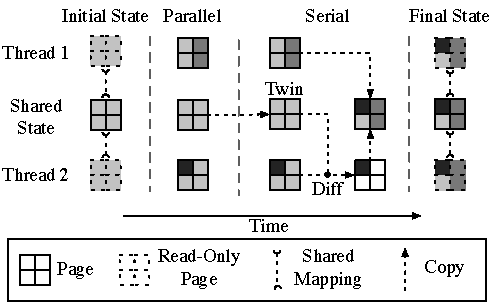
\includegraphics[width=6in]{dthreads/figure/architecture-diagram}
\caption{An overview of \dthreads{} execution.\label{fig:architecture}}
}
\end{figure}

\dthreads{} employs the following mechanisms to ensure the deterministic execution, illustrated by Figure~\ref{fig:architecture}: 

\textbf{Isolated Memory Access:} In \dthreads{}, threads are actually running as separate processes with private and shared views of memory, which is based on the \sheriff{} framework. Because processes have separate address spaces, \dthreads{} can isolate executions of different ``threads''. \dthreads{} uses this isolation mechanism to control the visibility of memory state, so that the updates made by a thread can not be seen by other threads if those updates are not committed explicitly to the shared mapping. By doing this, we guarantee that each ``thread'' can operate independently until synchronization points. Implementation of this is discussed in depth in Section~\ref{sec:threadsasprocs}.

\textbf{Deterministic Memory Commit:} 
Multithreading programs use shared memory for communication, thus \dthreads{} must propagate a thread's changes to be seen by other threads. To guarantee determinism, \dthreads{} should publish updates of different threads in a deterministic order at deterministic points.

\dthreads{} actually commits the changes of a thread to the shared state in sequence at synchronization points. These points includes thread creation and exit; mutex lock and unlock; condition variable wait and signal; posix sigwait and signal; and barrier waits. Commits are ordered using a global ``token'' that is passed from one thread to the next; a thread can only commit when it holds the token.  The token-passing protocol is described in Section~\ref{sec:schedule} and the implementation of synchronization primitives is described in Section~\ref{sec:synchronization}.

\dthreads{} relies on the twinning and diffing mechanism to find out local changes of different threads, which has been discussed in Section~\ref{sec:twinning-and-diffing}. 

\textbf{Deterministic Synchronization:}
There is no deterministic guarantee on synchronizations under existing operating systems. Thus, \dthreads{} re-implements the full range of pthreads synchronization primitives and discusses  them in details in Section~\ref{sec:synchronization}. 

\hspace{1em} \\
\noindent
\textbf{Fixing the data race example} \\
About the example program in Figure~\ref{fig:nondeterminism},  \dthreads{} effectively isolates the execution from each thread until it completes, and then orders updates from different threads by thread creation time using a deterministic last-writer-wins protocol.

In the beginning of every execution, thread 1 and thread 2 have the same view of shared state, with a = 0 and b = 0. Because changes by one thread to the value of a or b will not be made visible to the other until this thread exits, both checks on two threads on line 2 will be true. Thread 1 sets the value of a to 1, and thread 2 sets the value of b to 1. These threads then commit their updates to the shared state and exit, with thread 1 always committing before thread 2. The main thread then should always prints “1, 1” on every execution.

This determinism not only enables record-and-replay and replicated execution, but also effectively converts Heisenbugs into “Bohr” bugs, making them reproducible. In addition, \dthreads{} optionally reports any conflicting updates due to racy writes, further simplifying debugging.


\section{Applications}
\label{sec:applications}

\subsection{Shared Mechanisms}
Before the description of different applications, we listed some shared mechanisms that are used by one or multiple applications. 

\subsubsection{Canary}
\label{sec:canary}
Canary was first proposed by StackGuard~\cite{StackGuard} to find stack smashing problems by placing a canary word before the return address on stack. Those attempts to overwrite the return address should corrupt the canary word at first. Canaries are borrowed to detect buffer overflow ~\cite{overflow:purify}. They are initialized to a special value in the beginning so that modifications of those values indicates the problems. Detection tools can place canary values anywhere in heap memory. \doubletake{} introduces a bitmap to track the locations of canary values, and can check for canaries that have been overwritten. Buffer overflow detection places canary values between heap objects to detect out-of-bounds writes, and use-after-free detection fills freed objects with canaries to detect writes through dangling pointers.

\subsubsection{Watchpoints}
\label{sec:watchpoints}
Watch point mechanism relies on hardware debug registers to monitor memory accesses on specific addresses. Previous work has used this mechanism for their specific targets ~\cite{fastboundschecking, Kivati}. The main target of debug registers is to support software debuggers, e.g. gdb. A small number of watchpoints are available on modern architectures (four on x86). Each watchpoint can be configured to pause program execution when a specific byte or word of memory is accessed. \doubletake{} allows detection tools to set hardware watchpoints before re-execution. Heap Overflow detection tool can use watchpoints to find the instruction(s) responsible for overwriting a canary value.

\subsection{Applications}
\label{sec:applications}

\doubletake{} implements three important applications based on its lightweight dynamic analysis framework. Those applications are implemented in a best-effort way to show the efficiency of our framework. They are not targeted for a complete and novel solution, thus most of mechanisms are borrowed from previous work. 

\begin{figure}[!t]
\begin{center}
\includegraphics[width=3.3in]{doubletake/figure/buffer-overflow-diagram}
\end{center}
\caption{Heap organization used to provide evidence of buffer overflow errors. Object headers and unrequested space within allocated objects are filled with canaries; a corrupted canary indicates an overflow occurred.
\label{fig:buffer-overflow}}
\end{figure}

\begin{figure}[!t]
\begin{center}
\includegraphics[width=3.3in]{doubletake/figure/dangling-pointer-diagram}
\end{center}
\caption{Evidence-based detection of dangling pointer (use-after-free) errors. Freed objects are deferred in a quarantine in FIFO order and filled with canaries. A corrupted canary indicates that a write was performed after an object was freed.
\label{fig:dangling-pointer}}
\end{figure}


\subsubsection{Detection of Heap Buffer Overflows}
\label{sec:overflow}
Buffer overflows occurs when a program writes outside of the range of an allocated object. Buffer overflows can greatly affect the reliability and security of a program. 

\paragraph{Detection.}
To detect heap buffer overflows, \DoubleTake{} puts canaries before and after actual heap objects, which is described in Figure~\ref{fig:buffer-overflow}. This method is borrowed from previous work~\cite{overflow:lbc, AddressSanitizer}.
All heap objects of \doubletake{} are managed by power of two size, adding two words for canaries (16 bytes) for each heap object. For an allocation size not power of two size (a non-aligned object), \doubletake{} rounds it up to the next power of two size class, putting byte-based canaries and word-based canaries immediately after this object. This approach lets \doubletake{} catch overflows as small as one byte. 

Detection happens in the following scenario. At memory deallocation, \doubletake{} checks buffer overflows only for non-aligned objects, with size different with the power of two class. At the end of each epoch, \doubletake{} verifies integrities of all canaries by traversing the bitmap, which marks the placement of canaries and discussed in Section~\ref{sec:canaries}.  Corrupted canaries indicates heap buffer overflows. 

\paragraph{Re-execution.}
\label{sec:overflowreport}
When a program is found to have heap overflows, \doubletake{} rolls back the execution to the most recent checkpoint and re-executes this program.
To precisely identifying instructions responsible for a buffer overflow, \doubletake{} installs a watch point at the address of a corrupted canary before re-execution. When the program is re-executed, any instruction that writes to this address will trigger a debug trap (resulting in a SIGTRAP signal). \doubletake{} then reports the exact call site of trapped instructions, acquired by calling \texttt{backtrace} function. To further help programmer, \doubletake{} can also report the allocation site of an overflowed heap object. 
  
\subsubsection{Detection of Memory Leak}
\label{sec:leak}
Heap memory is leaked when it becomes inaccessible without being freed. Memory leak can greatly reduce the performance and availability of programs, which makes it one of common classes of reported bugs.

\paragraph{Detection.}
\doubletake{} detects memory leak using the same marking mechanism as conservative garbage collection ~\cite{Wilson:1992:UGC:645648.664824}. \doubletake{} marks the reachability of all heap objects: whether a heap object is reachable from the globals, the stack, and registers. Any unreachable object that has not been freed must be leaked. 

In order to compute the reachability from globals, stack, and registers, \doubletake{} starts to put all possible pointers, any eight-byte aligned value falling into the range of the heap, into a work queue. Then \doubletake{} checks all values in the queue using a breadth-first search algorithm: for each value, \doubletake{} verifies whether this value is a valid address inside a heap object; If this valid object is still non-reachable (not checked before), \doubletake{} marks it as reachable and also put all possible pointers inside this object into the work queue. After this step, this value is removed from the work queue. \doubletake{} stops when there is no value in the work queue any more. In this time, all heap objects which is reachable should have been marked. 

After the marking phase, \doubletake{} traverses the whole heap to find leaked objects, those un-reachable non-freed objects. To simplify the marking and checking phase, the status of an object, whether it is freed or reachable are marked in the object header. During this traverse, \doubletake{} recovers the status of every object to un-reachable. \doubletake{} also adds all leaked objects into a global hash table, where each leaked object also keeps information of its starting address and size. 

\paragraph{Re-execution.}
\label{sec:leakreport}
\doubletake{} uses re-execution to find allocation sites for all leaked heap objects. Re-execution proceeds as normal, with an added check in each \texttt{malloc()} function call. When a memory allocation matches the actual size and address of any leaked heap object, 
\doubletake{} reports its call stack, obtaining by using \texttt{backtrace} 
functions of \texttt{glibc} library. 

\subsubsection{Detection of Use-after-free Errors}
\label{sec:danglingpointer}
Memory use-after-free errors occur when an application continues to use a pointer after its corresponding object has been deallocated.
Writing to a freed memory can overwrite the contents of lived objects, leading to unexpected behavior.  

\paragraph{Detection.}
To detect memory use-after-free errors, 
\doubletake{} firstly delays memory re-usage of all freed objects 
by putting them into a quarantine list, same as AddressSanitizer does ~\cite{AddressSanitizer}. 
Those objects in the quarantine list are actually returned back
to the program heap when the total size of freed objects in the quarantine list are larger then a pre-defined threshold or the quarantine list is full.

In order to find evidence of memory use-after-free problems, 
\doubletake{} fills the first 128 bytes of an object, which can be adjustable, with canaries. 

Those canaries are checked before an object is returned back to the program heap or in the end of an epoch. Same as detection of buffer overflows, 
a corrupted canary indicates a use-after-free memory error and must be reported to user. 

\paragraph{Re-execution}
When a program has use-after-free memory errors, \doubletake{} re-executes this program to find out the allocation and deallocation site of corresponding objects and those instructions actually writing them.
%It is possible that multiple instructions can access an object after deallocation.  

To obtain an object's call site of allocation and deallocation, 
\doubletake{} checks starting address of each object during every memory allocation and deallocation. If an object has the same address as those use-after-free objects, its corresponding allocation/deallocation site are saved. To find out those instructions writting a freed object, 
\doubletake{} installs hardware watch points on those violating addresses, which shares the same mechanism as overflow detection.
\doubletake{} reports an use-after-free error, with its allocation site and deallocation site, in order to help programmers locate a memory use-after-free error. 

\section{Implementation}
\label{sec:implementation}

\doubletake{} is implemented as a library and can be linked directly to programs, or can be injected into unmodified binaries by setting the \texttt{LD\_PRELOAD} environment variable on Linux.

At startup, \doubletake{} begins a new epoch. The epoch continues until the program issues an \emph{irrevocable} system call (see Section~\ref{sec:syscalls} for details). Before this call is issued, \doubletake{} scans program state for evidence of errors. The details of this scan are presented in Section~\ref{sec:applications}.

If no errors are found \doubletake{} ends the epoch, issues the irrevocable system call, and begins a new epoch. If any detection tools have found evidence of an error, \doubletake{} enters re-execution mode. The remainder of this section describes the implementation of \doubletake{}'s core functionality.

\subsection{Epoch Start}
\label{sec:implementation/start}

At the beginning of each epoch, \doubletake{} takes a snapshot of program state. \doubletake{} saves all writable memory (stack, heap, and globals) from the main program and any linked libraries, and saves register state of each thread with the \texttt{getcontext} function. Read-only memory does not need to be saved. To identify all writable mapped memory, \doubletake{} reads the Linux \texttt{/proc/self/map} file. \doubletake{} also saves file positions of all open files. This lets programs issue \texttt{read} and \texttt{write} system calls without ending the current epoch. \doubletake{} uses the saved memory state and file offset to ``undo'' these calls if the epoch needs to be re-executed when an error is found.

%%%%%%%%%%%%%%%%%%%%%%%%%%%

\subsection{Normal Execution}
\label{sec:implementation/normalexecution}

Once a snapshot has been saved, \doubletake{} lets the program execute normally. Most program operations proceed normally, but \doubletake{} interposes on heap allocations and system calls in order to set tripwires and support re-execution.

%%%%%%%%%%%%%%

\subsubsection*{System Calls}
\label{sec:syscalls}
\begin{table}[t]
	\centering
	\small
	\renewcommand{\arraystretch}{1.5}
	\begin{tabular}{l|p{6cm}}
		\textbf{Category} & \textbf{Functions} \\
		\hline
		
		Repeatable		& \texttt{getpid}, \texttt{sleep}, \texttt{pause}\\
		
		Recordable		& \texttt{mmap}, \texttt{gettimeofday}, \texttt{time}, 
						  \texttt{clone} , \texttt{open}\\
		
		Revocable		& \texttt{write}, \texttt{read} \\
		
		Deferrable		& \texttt{close}, \texttt{munmap} \\
		
		Irrevocable		& \texttt{fork}, \texttt{exec}, \texttt{exit}, \texttt{lseek}, \texttt{pipe}, \texttt{flock}, \texttt{socket related system calls}\\
	\end{tabular}
	\caption{System calls handled by \doubletake{}. All unlisted system calls are conservatively treated as irrevocable, and will end the current epoch. Section~\ref{sec:syscalls} describes how \doubletake{} handles calls in each category.\label{table:syscalls}}
\end{table}

\doubletake{} ends each epoch when the program attempts to issue an irrevocable system call. However, most system calls can safely be re-executed or undone prior to re-execution. 

\doubletake{} breaks system calls into five categories, shown in Table~\ref{table:syscalls}. System calls could be intercepted using \texttt{ptrace}, but this would add unacceptable overhead during normal execution. Instead, \doubletake{} interposes on all library functions that may issue system calls.

%%%%%%%

\emph{Repeatable system calls} do not modify system state, and return the same result during normal execution and re-execution. No special handling is required for these calls.

\begin{figure*}[ht!]
	\begin{center}
		\includegraphics[width=6.5in]{figure/perf}
	\end{center}
	\caption{Runtime overhead of \doubletake{} (OD = Buffer Overflow Detection, LD = Leak Detection, \doubletake{} = all three detections enabled) and AddressSanitizer, normalized to each benchmark's original execution time. 
%Overhead for Valgrind is reported in Table~\ref{table:valgrind} because the results do not fit on this graph.
\label{fig:perf}}
\end{figure*}

%%%%%%%

\emph{Recordable system calls} may return different results if they are re-executed. \doubletake{} records the result of these system calls during normal execution, and returns the saved result during re-execution. Some recordable system calls, such as \texttt{mmap}, change the state of underlying operating system. Memory mapped with a call to \texttt{mmap} is left mapped for the entire epoch's re-execution; this is safe because the program cannot access this memory until the point at which the \texttt{mmap} call is replayed.

\emph{Revocable system calls} modify system state, but \doubletake{} can save the original state beforehand and restore it prior to re-execution. Most file I/O fall into this category.

For example, \texttt{write} modifies file contents, \doubletake{} can write the same content during re-execution. \texttt{write} also changes the current file position, which \doubletake{} restores to the saved file position using \texttt{lseek} prior to re-execution. \doubletake{} saves all file descriptors of opened files in a hash table at the beginning of each epoch. In addition, \doubletake{} must save stream contents returned by \texttt{fread}. Calls to \texttt{read} and \texttt{write}  on normal files, which can be identified by check the hash map, don't need to be handled. But those calls on socket files are treated as irrevocable system calls.
	
\emph{Deferrable system calls} will irrevocably change program state, but can safely be delayed until the end of the current epoch. \doubletake{} delays all calls to \texttt{munmap} and \texttt{close}, and executes these system calls before exiting or starting a new epoch.
	
\emph{Irrevocable system calls} change internally-visible program state, and cannot be undone. \doubletake{} must end the current epoch before these system calls are allowed to proceed. Note that for \doubletake{}, the meaning of ``irrevocable'' is different from that used in transactional memory systems~\cite{Irrevocabletrans}. Unlike in transactions, we expect re-execution to be identical to the epoch's original execution. It is safe for system calls to affect externally-visible state as long as the effect on internal state can be hidden or undone.

Note that in the presence of multiple threads, an error may fail to appear in the re-execution because of data races (synchronization ordering is already tracked and replayed). \doubletake{} then re-executes the code in an attempt to reveal the error. If it fails to reveal the error on replay, \doubletake{} has effectively tolerated the error and continues execution.

%%%%%%%%%%%%%%

\subsubsection*{Multithreaded Support}
We have implemented support for multiple threads, but the recording and re-execution of thread synchronizations is not yet stable. \doubletake{} records the sequence of system calls and results separately for each thread.

Every mutex records the order of threads that acquire it, and condition variables record the order of thread wakeups. \doubletake{} does not enforce a total global order on lock acquisitions. Operations within a single thread are totally-ordered, and \doubletake{} enforces local order at each synchronization point. In the absence of data races, this is sufficient to ensure deterministic re-execution.

Calls to \texttt{pthread\_create} are recorded with the same mechanism as recordable system calls. When a new thread starts, \doubletake{} takes a snapshot of the thread's stack and registers to enable re-execution from the beginning of the thread's execution. As with synchronization operations, \doubletake{} logs thread creation order and enforces this order during re-execution. Calls to \texttt{pthread\_exit} are deferred until the end of the epoch. Because \texttt{pthread\_exit} is deferred, \texttt{pthread\_join} is effectively deferred as well.

%%%%%%%%%%%%%%

\subsubsection*{Heap Allocator}
\label{sec:heapallocator}

Heap allocators typically issue a large number of \texttt{mmap} or \texttt{sbrk} system calls, which would complicate \doubletake{}'s logging re-execution. \doubletake{} replaces the default heap with a fixed-size BiBOP-style allocator with per-thread subheaps and power-of-two size classes, built using Heap Layers~\cite{heaplayers}. \doubletake{}'s heap is completely deterministic, so no logging is required to ensure that allocations do not change during re-execution.

When an object is freed, the allocator checks which subheap it is allocated from. If the object comes from the freeing thread's subheap, the \texttt{free} call proceeds uninterrupted. If the object was originally allocated by a different thread, the \texttt{free} is deferred. When the epoch ends, each object whose \texttt{free} was deferred is returned to its source thread's freelist.

During replay, \doubletake{}'s heap allocator checks to see if the object being allocated or freed contains the address where an error was detected. If so, \doubletake{} calls the \texttt{backtrace()} function to obtain a call stack for the allocation and deallocation sites.

\doubletake{} lets error detection tools traverse the set of all allocated objects during error checking. Objects are marked as allocated in object headers, including a size of the \emph{requested size}, which may be less than the power-of-two size class for object. All three detection tools use this size during scanning.

\doubletake{} also maintains a bitmap to record the locations of heap canaries. The bitmap records every word of heap memory that contains a canary. \doubletake{} notifies the detection tool when any of the bytes do not contain canaries. Buffer overflow detection places canaries only outside the requested object size. Re-execution is only started if the detection tool finds that canaries between allocated objects have been overwritten.

%%%%%%%%%%%%%%

\subsubsection*{Epoch End}

The epoch ends when any thread issues an irrevocable system call. All other threads are notified with a signal. Once all threads have stopped, \doubletake{} checks the program state for errors. The application-specific error checks are described in Section~\ref{sec:applications}. If an error is found, \doubletake{} immediately switches to re-execution mode. If not, the runtime issues any deferred system calls and clears the logs for all recorded system calls.

%%%%%%%%%%%%%%%%%%%%%%%%%%%

\subsection{Re-Execution}
\label{sec:implementation/re-execution}

Before re-executing the current epoch, \doubletake{} must roll back program state. Restoring saved memory will overwrite the current stack, so \doubletake{} switches to a temporary stack during rollback. The saved state of all writable memory is copied back, and any revocable system calls are undone (see Section~\ref{sec:implementation/normalexecution} for details). Before restoring register state, \doubletake{} must allow detection tools to place watchpoints.

\subsubsection*{Watchpoints}
Debug registers are not accessible in user-mode, so \doubletake{} must use \texttt{ptrace} to set watchpoints. \doubletake{} forks a child process and attaches to it using \texttt{ptrace} to load watched addresses into the debug registers and enable the watchpoints.

Once watchpoints have been placed, \doubletake{} uses the \texttt{setcontext} call to restore register state and begin re-execution. During re-execution, \doubletake{} replays the saved results of system calls from the log collected during normal execution. All deferred system calls are converted to no-ops while the program is re-executing.

\subsection*{Synchronization Replay}
\doubletake{} enforces the recorded order of synchronization operations during re-execution. A thread can only acquire a mutex if it is the next thread in the acquisition log, regardless of whether the mutex is currently locked. \doubletake{} uses semaphores to wake threads from condition variables in the recorded order. When a condition variable is signaled, the signaling thread notifies next waking thread that it can resume. If this thread has not yet arrived at the condition variable, it will wake immediately after it arrives.


%\section{\doubletake{} for Multithreading Programs}
%\label{sec:multithreading}

This section describes the mulithreading support of \doubletake{}.
A thread is a basic execution unit from the point of view of underlying operating system. 
The order of an execution, greatly affecting memory usage, 
is highly depending on timing, synchronization order and internal scheduling algorithm.   
Thus, it is much more difficult to achieve the target of repeatable memory 
usage for multithreading programs, which is crucial to 
precisely detect buffer overflows or other memory errors.
This section first discusses how to handle epochs in multithreading programs.
After this, it describes the design of heap allocator, suitable for repeatable memory usage.
It then discusses how to handle thread creation and exits specially. 
In the end, it describes how to guarantee deterministic synchronization in the re-execution phase,
which is also crucial for repeatable memory usage.


\subsection{Overview}
\label{sec:mtoverview}

As described in Section~\ref{sec:overview}, \doubletake{} uses irrevocable system calls as 
boundaries for epochs for multithreading programs. 
To simplify description in the following sections, a thread encountering an irrevocalbe system call is 
called as the ``Triggering-Thread''. 

When encountering an irrevocable system call, this Triggering-Thread 
has to stop all existing threads so that all other threads are in a quiecent state, which
has been described in Section~\ref{sec:stopepoch}.
Then it performs memory checkings on the heap as described in Section~\ref{sec:epochend}. 
If there is no buffer overflow, it can perform this irrevocable system call and 
start a new epoch after this system call. 
Before waking up other threads, the Triggering-Thread takes a snapshot for the shared memory at first,
including the heap and globals. 
After a thread is waken up, it only needs to take a snapshot on its own state, 
including its stack and its hardware registers. 

If there are buffer overflows, the Triggering-Thread sets up the shared memory 
for all threads at first.
It recovers the heap and globals by copying from the saved snapshot. 
Then it can wake up other threads. 
However, if the Triggering-Thread is spawed newly in current epoch, 
it has to wait for its parent to start its execution. 

\subsubsection{Epoch}
\label{sec:stopepoch}

It is the duty of a Triggering-Thread to close an epoch.
Whenever this thread meets an irrevocable system call, it has to stop other threads.
\doubletake{} utilizes the ``signal'' mechanism to stop other threads asynchronously.
It signals other threads using SIGUSR2 signal when a thread is in a safe state. 
A thread is considered to be in a unsafe state before this thread finishs a snapshot for itself,
discussed in Section~\ref{sec:threadcreation}.
After sending out all signals, this thread is waiting on a internal conditional variable.
The Triggering-Thread only starts checking buffer overflows after all threads are in quiescence.

However, this SIGUSR2 signal can also be used by user programs. 
In order to differentiate this, \doubletake{} specifically marks on 
a shared flag before signalling so that signal handler can check this in the beginning. 
If this flag is marked, this signal is issued by \doubletake{}. Otherwise, it is issued by
a user program and we can call user registered program instead. 

When other threads receive the signal from the Triggering-Thread, 
they are waiting on an internal conditional variable for instructions from the Triggering-Thread:
it can move forward to next epoch or rollback.
It is worthy noting that inside signal handler we have to utilize a different lock that has not been
used by other places. Otherwise, it is easy to cause deadlock. 

\subsubsection{Customized Heap Allocator}
\label{sec:mtheap}
In order to achive the target of repeatable memory usage, the heap allocator must be designed 
carefully. \doubletake{} first borrows a ``per-thread-heap'' idea from Hoard~\cite{Hoard}. 
\doubletake{} keeps a 1-to-1 mapping between threads and sub-heaps of customized memory allocator. 
The total number of threads and sub-heaps are pre-defined. 
A thread can only allocate memory from its own sub-heap, 
where those sub-heaps can get the memory from a pre-allocated heap 
by allocating a huge block of memory each time. 
After a sub-heap gets a block of memory, its corresponding thread always owns all objects
of this block, called as ``owner'' of this block.
This surely can cause memory blowup problem resolved by Hoard. However, it is 
not the focus of \doubletake{}.   

The ``per-thread-heap'' idea is not enough to guarantee the repeatable memory usage. 
\doubletake{} imposes several additional rules besides this.
Firstly, when \doubletake{} acquires a block of memory from the global pre-allocated heap, it must 
acquire a lock at first, which is guaranteed to be deterministic according to mechanisms 
discussed in Section~\ref{sec:sync}.
This guarantee that every new blocks of each sub-heap is repeatable for re-execution. 
Secondly, when there is a memory deallocation, this freed object can only be returned back  
to its original owner in a safe state. 
If this memory deallocation is issued by the same thread as the owner, then this freed object
can be putted into the owner's free list and be utilized immediately. 
If this memory deallocation is issued by a different thread with the owner, 
which indicates a cross-thread communication,  
then this memory
deallocation are cached into a global list, which only issued in the end of this epoch after 
all threads has been stopped. 
By doing this, we can guarantee all memory usage inside an epoch is repeatable in re-execution phase.
 
\subsection{Thread Creation and Exit}
\label{sec:threadcreation}
Tracking creations and exits of threads is very important because of the following reasons.
First, \doubletake{} has to take snapshots for different threads in the beginning. 
Second, terminination of a thread invokes \texttt{munmap} system calls directly by \pthreads{}, which
can not be intercepted.  
Third, thread creation is considered as a synchronization and has to be recorded. 
Thus, \doubletake{} intercepts \texttt{pthread\_create} calls and changes its start routine 
to a customized function. 
In this customized function, \doubletake{} can record thread creation, take a snapshot and delay thread exit to the end of current epoch. 

\subsubsection{Normal Execution}

\doubletake{} makes \texttt{pthread\_create} to call its customized function as the start routine. 
In this start routine, \doubletake{} first puts this new thread into a global map, which maintains
status of all threads. 
Then it takes a snapshot for this new thread, including stack and hardware registers. 
After this, \doubletake{} can invoke the original routine to actually perform user-defined 
thread function. 

After this user-defined thread function finishes, the control flow returns back to \doubletake{}. 
Basically, \doubletake{} should check whether this thread's parent is joining on this thread or not. 
If this thread's parent is already waiting for its termination, it simply marks the status of 
this thread to be joined and wakes up the joining thread. 
If not, this thread can wait on a thread-private conditional variables. 
\doubletake{} delays a thread exit to the end of current epoch.

\subsubsection{Re-execution}
A thread is waiting for its turn to run if a thread is created in current epoch.    

\subsection{Thread Synchronizations}

\label{sec:sync}

Different order of thread synchronizations can lead to totally different memory uage. 
In order to guarantee deterministic replay of thread synchronizations, previous work
actually forces threads to do synchronizations in a global order and
recordes both lock and unlock operations ~\cite{TERN, PRES}. 
However, forcing a global order of synchronizations can greatly 
reduce parallelism and introduce significant performance overhead.
Also, it is unnecessary to record unlock order too.

Unlike previous approaches, \doubletake{} only records local orders of synchronizations.
Synchronizations on two different synchronization variables can be performaed
in parallel. From a thread's point of view, if a program do not have a race and
all synchronizations of a thread are repeated deterministically, then
\doubletake{} can guarantee memory usage of this thread, which also guarantees to 
repeat the same buffer overflows in re-execution phase. 
If a program do have a race, forcing a global order of synchronizations in the production 
run also can not completely avoid races. This also implies that a global order 
can not always guarantee determinstic memory uage.   
\doubletake{} prefers performance for racey programs, while relying on multiple re-executions 
to repeat buffer overflows if a program does have a race problem. 

\doubletake{} records the order of \texttt{pthread\_mutex\_lock}, conditional wakenup and
different signalling functions.
Signalling functions actually calls system calls, which are handled by the procedure discussed 
in Section~\ref{sec:inepoch}.
 Conditional wakenup is actually related to \texttt{pthread\_cond\_wait},
which actually includes conditional wait and conditional wakenup phases. 
Conditional wait atomically releases mutex and waits on corresponding conditional variable, while conditional wakenup actually locks corresponding mutex before returning. 
Thus, we can turn \texttt{pthread\_cond\_wait} to two operations, \texttt{pthread\_mutex\_unlock} and
\texttt{pthread\_mutex\_lock} correspondingly. So we only record the order of conditional wakenup in
production runs. 
 
\doubletake{} also provides an option to record the order of passing a specified barrier, which it is 
not necessary to do this by default.
It is noted that \doubletake{} do not record the order of unlock operations
and conditional signal operations.
It is totally unnecessary to record unlock operations since recording the order of actual 
lock aquiring operations is enough to guarantee a deterministic replay of critical sections.  
Conditional signal and broadcast operations are skiped for the same reason. 

%why two different synchronization is not important?
How to replay this?
How to handle nested locks? 
The replaying is considerred to be two steps: we first advance thread's entry when we met a .

Maybe pseudo code for this.
 
\subsubsection{Normal Execution}
In production runs, \doubletake{} intercepts all synchronizations and 
records orders of synchronizations, such as lock, conditional waken up and signals, 
based on different synchronization variables. 
It maintains a list for each synchronization variable and records synchronization
events on its corresponding list. 
In order to quickly locate its list when a synchronization is intercepted, \doubletake{}
utilizes original synchronization variables to store addresses of list and actual synchronization
variable. 

For a synchronization event like lock, \doubletake{} records the following information:
which thread issues this synchronization event; what is the result of this synchronization.
A naive implementation is to allocate memory from internal memory allocator every time. 
However, for some applications having significant amount of synchronizations,
memory allocations to record synchronization events contributes much performance overhead. 
For example, \texttt{fluidanimate} runs several times slower because of huge amounts
of synchronizations inside. \doubletake{} uses a pre-allocated list for those recordings. 
More specifically, each thread has a pre-allocated list in the beginning of an epoch. 
When a synchronization occurs on this thread, it can get an entry from this thread and 
record a synchronization event on this entry.
Since \doubletake{} always gets an entry from current thread issuing a synchronization,
there is no need to utilize a lock, which also helps reducing overhead. 
By doing this, \doubletake{} greatly reduce performance overhead of logging synchronization
events. For example, performance overhead of \texttt{fludidanimate} are reduced to around 40\%.

 
\subsubsection{Re-execution}
As described above, for a synchronization event in a thread,
\doubletake{} allocates an entry from current thread to record this synchronization event 
and inserted it into synchronization variable's corresponding list. 
This implies that a synchronization event belongs to two lists, 
a list for all synchronizations of this synchronization variable (SyncVariableList) and 
a list for all synchronizations in a thread (ThreadSyncList). 

Reproducing synchronizations involves in manipulating these two lists using 
{\it sempaphore replay}, similar to TERN ~\cite{TERN}.
We listed the pseudocode of ``lock'' of reproduction runs in Figure~\ref{fig:lockunlock}.
\doubletake{} assigns a semaphore for each thread and controls the order 
of synchronizations based on semaphores: in lock acquisitions, 
a thread waits on its semaphore and advances ThreadSyncList after this semaphore; 
In lock releases, a thread increments the semaphore of next thread on the same 
synchronization variable.
However, \doubletake{} only records local synchronization order, instead of global order,
synchronizations replaying of \doubletake{} is much more subtle.
In order to handle those unsuccessful lock acquisitions, \doubletake{} only waits for a semaphore 
if this lock is successfully acquired in the production run. 
Also, to support nesting locks, in lock acquisitions after {\it advanceThreadSyncList()}, 
\doubletake{} signals current thread if next event of this thread is already 
in its pending list, which means that this thread should have its turn.
For lock releases, \doubletake{} adds next event of SyncVariableList to corresponding thread's 
pending list if the event is not the first event of corresponding thread instead of incrementing
its semaphore directly. 
Since performance of reproduction runs is not the main focus, only occurring for those programs 
having buffer overflows, \doubletake{} are using the same lock for all lists' manipulations to
avoid races.  




%\section{Optimization}
%\input{optimization}

\section{Evaluation}
\begin{figure*}[htb]
{\centering
\tiny
\subfigure{\lstinputlisting[numbers=none,frame=none,boxpos=t]{predator/figure/linearregression.report}}
\caption{An example report by \Predator{} indicating false sharing in the linear\_regression benchmark.
\label{fig:lrreport}}
}
\end{figure*}



\label{sec:evaluation}

This section answers the following questions:
\begin{itemize}
\item
  How effective is \Predator{} at detecting and predicting false sharing?

\item
  What is \Predator{}'s overhead, in terms of execution time and memory ?

\item
  How sensitive is \Predator{} to different sampling rates?
 
\end{itemize}

\paragraph{Experimental Platform.} All evaluations are performed on a quiescent Intel Core 2 dual-processor system equipped with 
16GB RAM. Each processor is a 4-core 64-bit Intel Xeon running at 2.33 GHz, with a 4MB shared L2 cache and 32KB private L1 cache. The underlying operating system is an unmodified CentOS 5.5, running with Linux kernel version 2.6.18-194.17.1.el5. The glibc version is 2.5. 

\paragraph{Evaluated Applications.}
This paper evaluates two popular benchmark suites,
Phoenix (with large input) ~\cite{phoenix-hpca} and PARSEC (with simlarge input) ~\cite{parsec}. Even with unmodified LLVM-3.2, Facesim cannot be compiled successfully (having complaints on an undefined template) and Canneal aborts unexpectedly. Thus, these two benchmarks are excluded.
We also evaluate \Predator{} on six real applications, including MySQL, Boost, Memcached, aget, pbzip2 and pfscan.



\subsection{Detection and Prediction Effectiveness}
\label{sec:effective}

For every false sharing problem, \Predator{} reports source code information and detailed memory access information in order to help users fix those problems. Figure~\ref{fig:lrreport} shows an example for the linear\_regression benchmark. This report shows that the heap object starting with $0x40000038$ potentially causes a large number of cache invalidations. The call stack of allocation is provided to help locate culprits. In addition, \Predator{} also reports word-level access information of this object, which helps to identify where and how false sharing occurs. From that, we can know that it is a latent false sharing problem predicted by \Predator{}, since different threads are accessing different cache lines. 

\subsubsection{Benchmarks}
\label{sec:benchmarks}

\begin{table*}[!t]
{\centering\begin{tabular}{l|r|r|r|r|r}\hline
{\bf \small Benchmark} & {\bf \small Source Code} & {\bf \small New} & {\bf \small Without Prediction} &{\bf \small With Prediction} & {\bf \small Improvement} \\
\hline
\small \textbf{histogram} & {\small histogram-pthread.c:213} & \cmark{} &\cmark{} & \cmark{} & 46.22\%\\
\small \textbf{linear\_regression} & {\small linear\_regression-pthread.c:133} & & & \cmark{} & 1206.93\% \\
\small \textbf{reverse\_index} & {\small reverseindex-pthread.c:511} & & \cmark{} & \cmark{} & 0.09\%\\
\small \textbf{word\_count} & {\small word\_count-pthread.c:136} & & \cmark{} & \cmark{} & 0.14\%\\
\hline
\small \textbf{streamcluster} & {\small streamcluster.cpp:985} &  & \cmark{} & \cmark{} &7.52\% \\
\small \textbf{streamcluster} & {\small streamcluster.cpp:1907} & \cmark{} & \cmark{} & \cmark{} & 4.77\%\\
\hline
\end{tabular}
\caption{False sharing problems in the Phoenix and PARSEC benchmark suites. \label{table:detection}}
}
\end{table*}

Table~\ref{table:detection} provides detection results of two benchmark suites, Phoenix and PARSEC
The first column lists those programs with false sharing problems.  The second column shows precisely where the problem is. Because all discovered false sharing occurs inside heap objects, we show callsite source code information here.  The third column, ``New'', marks whether this false sharing was newly discovered by \Predator{}.  A checkmark in the following two columns indicates whether the false sharing was identified without
prediction and/or with prediction.  The final column, ``Improvement'', shows the performance improvement after fixing false sharing.
%The number is based on the average runtime of $10$ runs. 

As shown in the table, \Predator{} reveals two unknown false sharing problems. It is the first tool to detect the false sharing problems in histogram and in line $1908$ of streamcluster. 
In histogram, multiple threads simultaneously modify different locations of the same heap object, thread\_arg\_t. 
Padding this data structure fixes the false sharing problem and improves the performance by around 46\%. In streamcluster, multiple threads are simultaneously accessing and updating the same \texttt{bool} array, switch\_membership. Simply changing all elements of this array to a long type reduces the false sharing and improves the performance by about 4.7\%.

%, although it is not a complete fix of false sharing. 
%None of these two false sharing problems has been reported by previous tools.
Other false sharing problems were discovered by previous work~\cite{sheriff}. We do not see significant performance improvement for reverse\_index and word\_count benchmarks. They are reported here because the number of cache invalidations in these two programs reaches our predefined threshold.
Making the reporting threshold higher can avoid the report of those insignificant false sharing problems.
It is worth noting that these two benchmarks definitely have false sharing problems,
which can be confirmed by word-level information generated by \Predator{}. 

The streamcluster benchmark has another false sharing problem at line $985$. Different threads change the work\_mem object simultaneously. Authors of streamclsuter have already realized this problem and provide a CACHE\_LINE macro. Unfortunately, the default value of this macro is set to $32$ bytes, which is different from the actual cache line size of the experimental machine. By setting it to $64$ bytes instead, it achieves  performance improvement of about 7.5\%.

linear\_regression has a severe false sharing problem. Fixing it improves the performance by more than $12\times$. In this benchmark, different threads update their thread-specific locations inside the tid\_args object in a tight loop. According to the observation of Nanavati et al., this false sharing problem occurs when using clang and disappears when using gcc with the -O2 and -O3 optimization level~\cite{OSdetection}. But we observed a different result when using the clang-3.2 compiler and our custom memory allocator: the false sharing problem does not occur at all because the offset of the starting address of the potentially falsely-shared object and the start of cache line is 56 bytes (see Figure~\ref{fig:perfsensitive}). With prediction mechanism, \Predator{} detects this latent false sharing problem, exemplifying the necessity of a predictive detection tool. 

\subsubsection{Real Applications}
To verify \Predator{}'s practicality, we further evaluate several widely-used real applications, whereas no previous work has done this. These real applications include a server application (MySQL~\cite{mysql}),
a standard C++ library (Boost~\cite{libfalsesharing}),
a distributed memory object caching system (Memcached), a network retriever (aget),
a parallel bzip2 file compressor (pbzip2), and a parallel file scanner (pfscan).

MySQL-5.5.32 and boost-1.49.0 are known to have false sharing problems. Other applications (memcached-1.4.15, aget-0.4.1 and pbzip2-1.1.6) do not have known false sharing problems.

The false sharing of MySQL has caused a significant scalability problem and was very difficult to identify.
According to the architect of MySQL, Mikael Ronstrom, ``we had gathered specialists on InnoDB..., participants from MySQL support... and a number of generic specialists on 
computer performance...'', ``[we] were able to improve MySQL performance by 6$\times$ with those scalability fixes''~\cite{mysql}. 
The false sharing inside Boost is caused by the usage of a  spinlock pool. Different threads may utilize different spinlocks located in the same cache line in this case. Fixing it brings a 40\% performance improvement.
\Predator{} is able to pinpoint false sharing locations in both MySQL and the Boost library. 
For the other four applications, \Predator{} does not find severe false sharing problems.

\subsubsection{Prediction Effectiveness}
\label{sec:predicteval}
In this section, we verify whether prediction can always  reveal un-observed false sharing problems.

The linear\_regression benchmark is selected here because of the following two reasons: (1) The false sharing problem of this benchmark cannot be detected without prediction; (2) False sharing severely degrades performance when it actually occurs. Hence, it is a serious problem that should always be detected. 

\begin{figure}[!t]
{\centering
\subfigure{\lstinputlisting[numbers=none,frame=none,boxpos=t]{predator/figure/linearregression.psedocode}}
\caption{The false sharing problem inside the linear\_regression benchmark: multiple threads simultaneously update their entries in lreg\_args.
\label{fig:linearregression}}
}
\end{figure}

Figure~\ref{fig:linearregression} shows the data structure and the source code exercising appropriate false sharing. The size of this data structure, lreg\_args, is $64$ bytes 
when the program is compiled to a $64$-bit binary. For this benchmark, the main thread allocates an array, containing as many elements as the number of underlying hardware cores. Each element is a lreg\_args type with $64$ bytes. This array is then passed to different threads (lreg\_thread function) so that each thread only updates its thread-dependent area. False sharing occurs if two threads happen to update data in the same cache line. 

Figure~\ref{fig:perfsensitive} shows how sensitive the performance is to different starting addresses of a falsely-shared object. When the offset is $0$ or $56$ bytes, this benchmark achieves its optimal performance and has no false sharing. When the offset is $24$ bytes, the benchmark runs around $15$ times slower than its optimal performance because of the false sharing problem.

Our evaluation shows that \Predator{} can always detect the false sharing problem with prediction enabled, demonstrating its effectiveness.

\subsection{Performance Overhead}
\label{sec:perfoverhead}

\begin{figure*}[!t]
\centering
\includegraphics[width=6in]{predator/figure/perf}
\caption{
Performance overhead of \Predator{} with and without prediction(PREDATOR-NP).
\label{fig:perf}}
\end{figure*}

To avoid the effect caused by extreme outliers, all performance data shown in Figure~\ref{fig:perf} is based on the average of $10$ runs, excluding the maximum and minimum values. 

For $16$ benchmarks from the Phoenix and PARSEC benchmark suites and six real applications, \Predator{} imposes $5.4\times$ performance overhead. There is no noticeable difference on performance whether the prediction mechanism is enabled or not. 
 
Among these programs, five of them, histogram, kmeans, bodytrack, ferret, and swaptions, have more than $8\times$ performance overhead. The histogram benchmark runs more than $26\times$ slower than original executions with \pthreads{} library, because tracking detailed access on cache lines with false sharing exacerbates the false sharing effect (see more discussion in Section~\ref{sec:sample}).  For bodytrack and ferret, although there is no false sharing, \Predator{} detects a large amount of cache lines with writes larger than {\it Tracking-Threshold}. Thus, tracking those accessing details for those cache lines imposes significant performance overhead. Currently, we cannot identify the reasons why kmeans runs very slowly on \Predator{}.
   
\Predator{} imposes a small performance overhead for IO-bound applications, such as matrix\_multiply, blackscholes, x264, aget, Memcached, pbzip2, and pfscan, since \Predator{} does not add any performance overhead for IO operations.  

\subsection{Memory Overhead}
\label{sec:memoverhead}
We only evaluate the physical memory overhead of \Predator{}, instead of the virtual memory overhead, because \Predator{} allocates four gigabytes virtual memory for its custom memory allocator. Proportional set size (PSS) in \texttt{/proc/self/smaps} reflects the physical memory increase on the existing system of running an application~\cite{memusage}. Thus, we periodically collect this data and use the sum of different memory mappings as the total physical memory usage of running an application. We present the maximum value of physical memory usage in Figure~\ref{fig:memusage}. 

\Predator{} imposes less than 50\% memory overhead for 17 out of 22 applications.  For swaptions and aget, \Predator{} introduces more memory overhead because the original memory footprints of them are very small, only $3$ kilobytes. Adding the code of detection, prediction and reporting contributes to a large ratio of memory overhead. We are not clear why MySQL consumes much more memory than others. Although the average memory usage of all applications is over $2\times$, the total memory usage overhead is only about $40\%$ on \Predator{}. 


\subsection{Sensitivity to Different Sampling Rates}
\label{sec:sensitivity}
In Section~\ref{sec:sample}, we discuss that \Predator{} utilizes the sampling mechanism to reduce the tracking overhead. Running an application with different sampling rates does not affect its memory usage. Thus, we only evaluate the effect of different sampling rates on performance and effectiveness. 

The default sampling rate used by \Predator{} is 1\%. In this section, we also evaluate two other sampling rates, 0.1\% and 10\%. The performance results under the three different sample rates are shown in Figure~\ref{predator/figure:sample}. \Predator{} introduces less performance overhead under a lower sampling rate, which meets our expectation. Concerning effectiveness, even using the 0.1\% sampling rate, \Predator{} can still detect all false sharing problems, but with a lower number of cache invalidations. Thus, different sampling rates do not affect the detection effectiveness.
 
\begin{figure*}[!t]
\centering
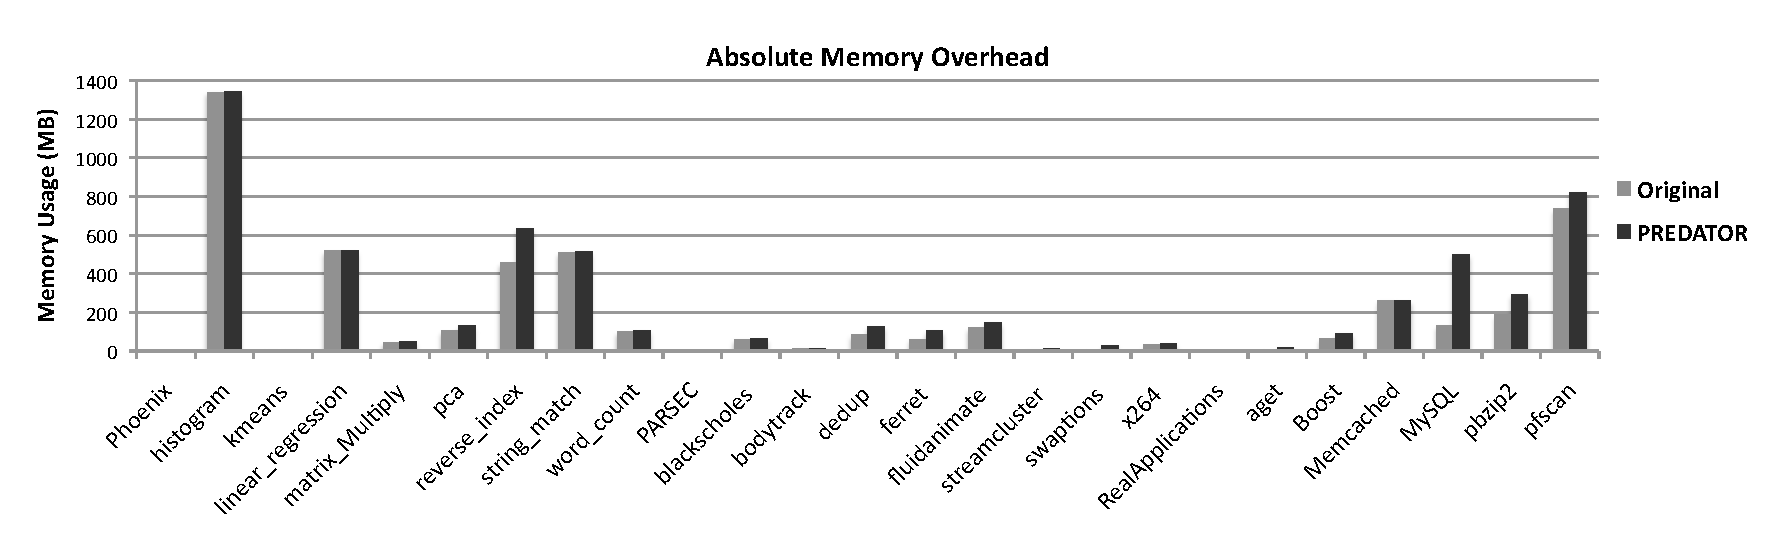
\includegraphics[width=6in]{predator/figure/absolutememory}
\caption{Absolute physical memory usage overhead with \Predator{}.}
\label{fig:absolutememusage}
\end{figure*}

\begin{figure*}[!t]
\centering
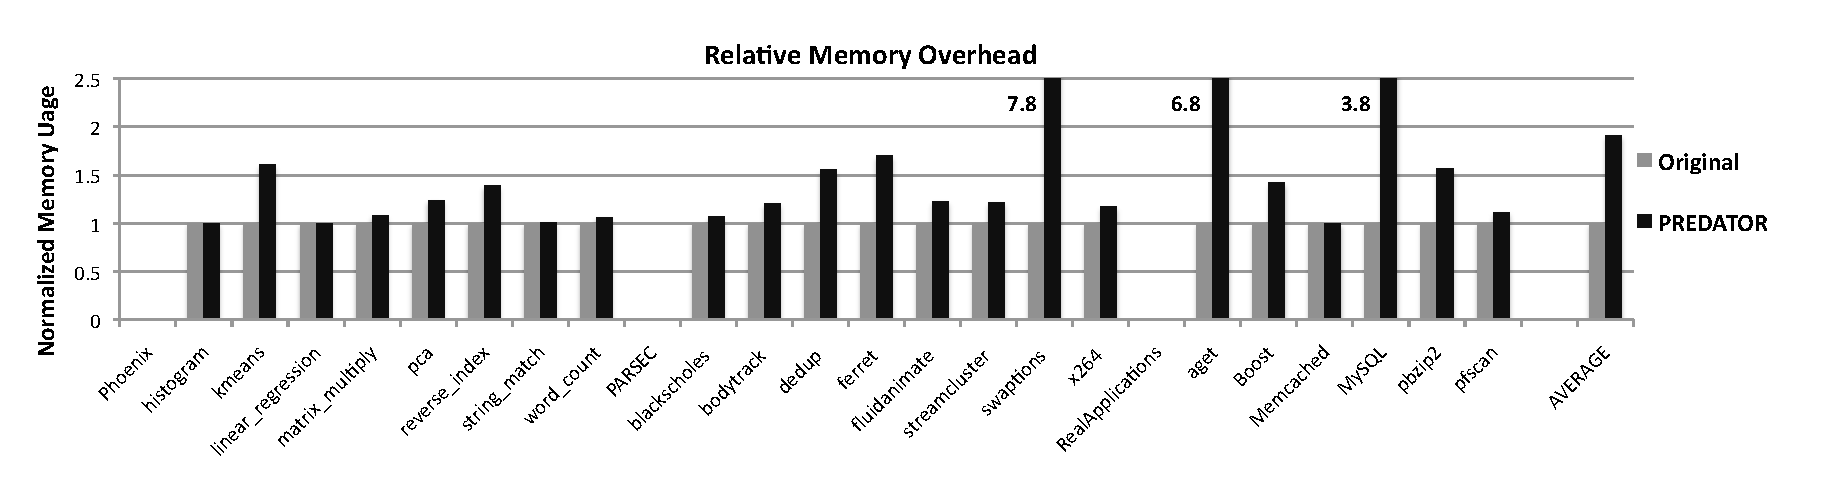
\includegraphics[width=6in]{predator/figure/memusage}
\caption{Relative physical memory usage overhead with \Predator{}.}
\label{fig:memusage}
\end{figure*}



\section{Discussion}
\label{sec:discussion}

This section analyzes some key limitations of \dthreads{} that
restrict its ability to run certain programs, limit the extent of
determinism it can guarantee, or potentially affect performance.


\textbf{Unsupported programs: }
\dthreads{} currently does not support programs with ad hoc
synchronizations, such as those that use atomic operations implemented in assembly.  However, the upcoming C++0X standard includes a library interface for atomic operations~\cite[pp. 1107--1128]{c++0xstandarddraft}, and a future version of \dthreads{} could correctly implement these by intercepting
these library calls and treating them as synchronization points. While
ad hoc synchronization is a common practice, it is also a notorious
source of bugs; Xiong et al.\ show that 22--67\% of the uses of ad hoc
synchronization lead to bugs or severe performance issues~\cite{ad-hoc-considered-harmful}.

\dthreads{} also currently does not write-share the stack
across threads, so that updates made by a thread to a stack variable
would not be reflected back to the parent, which could cause a program
to fail. Passing stack variables to a thread for modification is
extremely error-prone and generally deprecated, making this a rare
coding practice.

\textbf{External determinism: }
While \dthreads{} provides internal determinism, it does not
guarantee determinism when a program's behavior depends on external
sources of non-determinism, such as system time or I/O
events. Incorporation of \dthreads{} in the dOS framework, an OS
proposal that enforces system-level determinism, would provide full
deterministic execution, although this remains future
work~\cite{deterministic-process-groups}.

\textbf{Runtime performance: }
Section~\ref{sec:evaluation} shows that \dthreads{} can provide high
performance for a number of applications; in fact, for the majority of
the benchmarks examined, \dthreads{} matches or even exceeds the
performance of \pthreads{}. However, \dthreads{} could occasionally
degrade performance, sometimes substantially. One way it could do so
would be to exhibit an intensive use of locks (that is, acquiring and
releasing locks at high frequency), which are much more expensive
in \dthreads{} than in \pthreads{}. However, because of its determinism guarantees, \dthreads{} could allow programmers to greatly reduce their use of locks, and thus improve performance. Other application characteristics, also explored in Section~\ref{sec:performance}, can also impair performance
with \dthreads{}.


%  Since Surprise locking inside libraries. Not a limitation \emph{per
%  se} but definitely an issue that could surprise programmers.

% Draft can be downloaded from http://www.open-std.org/jtc1/sc22/wg21/docs/papers/2010/n3126.pdf.
%Fine once they are library calls, as they are in gcc and in the upcoming C++0X standard (cite!), since then we can intercept them.

\textbf{Memory consumption: }
Finally, because \dthreads{} creates private, per-process copies of
modified pages between commits, it can increase a program's memory
footprint by the number of modified pages between synchronization
points. This increased footprint does not seem to be a problem in
practice, both because the number of modified pages is generally far
smaller than the number of pages read, and because it is transitory:
all private pages are relinquished to the operating system
(via \texttt{madvise()}) at the end of every commit operation.

%Increased memory footprint (linear in the number of dirtied (modified) pages).




\section{Related Work}

\label{chapter:relatedwork}
This chapter first describes those related work to processes-as-threads framework and deterministic execution. Then it describes related work in false sharing detection, prevention, or both. 

\section{Processes-As-Threads framework}

BOP relies on strong isolation of processes to automatically and safely parallelize the execution of programs~\cite{DingBOP}. BOP forks a new process to do speculation, based on those pre-defined possibly parallel regions (PPR). In order to check the correctness, BOP tracks accesses on a page-based granularity. When there is no conflict and a speculative process reaches the end of its current PPR, its predecessor always commits its changes to the current process. However, BOP does not provide any synchronization support and can not be used to run normal multithreaded programs. 

Grace is a process-based approach designed to prevent
concurrency errors, such as deadlock, race conditions, and
atomicity errors by imposing a sequential semantics on
speculatively-executed threads~\cite{grace}. Grace supports only fork-join programs without inter-thread communication (e.g., condition variables or barriers), and rolls back threads when accesses of threads would violate sequential semantics: a thread accesses pages that have been accessed by its predecessors. Grace can not support arbitrary multithreaded programs. Similar to the Grace system, Sammati is a processes-as-threads system to detect and tolerate deadlock problems~\cite{Pyla:2010:ADA:1854273.1854288}. However, Sammati does not support the full range of synchronizations, without synchronizations, barriers, and signals. Also, Semmati can not avoid race conditions happening in creating twin pages, which are avoided by \Sheriff{} framework.

\begin{comment}
% Some usage of this framework
According to Revisions,  Grace cannot easily resolve all
conflicts on commit (like revisions do) and must thus restrict
tasks from producing such conflicts either statically (by type
system) or dynamically (pessimistic with blocking, or optimistic with abort and retry). Also, Grace allows only a restricted “fork-join” form of concurrency
Revisions~\ref{Burckhardt:2010:CPR:1869459.1869515}
\end{comment}

\section{Deterministic Multithreading}
The research on deterministic multithreading is a very active area these years. We describe some software-only, non- language-based approaches here.

\subsection{Software-only deterministic system}
Grace prevents deadlocks, race conditions, ordering and atomicity violations errors for those fork-join multithreaded programs by imposing a sequential semantics at join points~\cite{grace}. However, Grace does not support programs with interthread communications, such as conditional variables and barriers.

CoreDet is a compiler-based approach to 
support general-purpose multithreaded programs~\cite{Bergan:2010:CCR:1736020.1736029}. 
CoreDet instruments those memory read and write operations as long
as those operations can not be proved to be thread-local in static analysis. 
In the runtime phase, CoreDet divides the execution into 
alternating parallel and serial phases and guides all memory operations 
using a memory ownership table: only those owned locations can be accessed
in the parallel phases; all non-owned locations and synchronizations can only 
be accessed in the serial phases guided by a global token.
CoreDet guarantees deterministic execution for racy programs without memory errors,
but with very high performance overhead: 
averagely $3.5\times$ slower than those using \pthreads{} library.
In order to guarantee determinsim, 
CoreDet has to serialize \emph{all} external library calls without instrumentation.
CoreDet doesn not provide deterministic 
memory allocations, which can not guarantee determinism for programs with memory errors.  
% The use of synchronization points as commit boundaries also makes \dthreads{}
% code relatively \emph{robust}: when updates occur after a given number of 
% instructions retired (as in CoreDet and Kendo), it is impossible for 
% programmers to know when interleavings can occur. Such boundaries could vary 
% depending on the underlying architecture and would also be input-dependent, 
% meaning that slightly different inputs could lead to dramatically different
% thread interleavings. By contrast, \dthreads{} guarantees that only changes to
% the sequence of synchronization operations affect the order in which updates 
% are applied.
dOS~\cite{deterministic-process-groups} is an extension to CoreDet
that uses the same deterministic scheduling framework.  dOS 
supports deterministic communication for those threads and processes inside the same
deterministic process groups (DPGs) and handle those external non-determinism by recording and
replaying interactions across DPG boundaries. 

Determinator is a microkernel-based operating system that enforces
system-wide determinism~\cite{efficient-system-enforced}.
Determinator provides separate address spaces and supports interprocess
communications at explicit synchronizaton points. 
Determinator is a proof-of-concept system, which can not support the whole rage of
threads APIs and can not work on legacy programs.  

Some other works can only support limited determinism or need user annotation.
Kendo can only guarantee the determinism for race-free programs~\cite{1508256}. 
TERN~\cite{stable-deterministic} provides a best-effort system to 
apply memoized schedules for future runs with similar inputs. 
It can not guarantee the determinism for racy programs, as Kendo. 
Peregrine~\cite{peregrine:sosp11} is a system based on TERN, which tries to record
 memory accesses orders for racy portion and apply those schedules for future runs possibly.
However, both TERN and Peregrine do not support complete determinism (using a best effort)
and requires program annotations. 

\subsection{Hardware-related deterministic System}

\section{False Sharing}

This section describes related work in false sharing detection, prevention, or both. There is no previous
system to predict unobserved false sharing.

\subsection{False Sharing Detection}
Based on the SIMICS functional simulator, Schindewolf et al.\ designed a tool to report different kinds of cache usage information, such as cache misses and cache invalidations~\cite{falseshare:simulator}. Pluto relies on Valgrind dynamic instrumentation framework to track the sequence of memory read and write events on different threads, and reports a worst-case estimation of possible false sharing~\cite{falseshare:binaryinstrumentation1}.
Similarly, Liu uses Pin to collect memory access information, and reports total cache miss information~\cite{falseshare:binaryinstrumentation2}.
These tools impose about $100-200\times$ performance overhead.

Zhao et al.\ developed a tool based on DynamoRIO framework to detect false sharing and other cache contention problems
for multithreading programs~\cite{qinzhao}. 
It uses a shadow memory technique to maintain memory access history and detects cache invalidations based on the ownership of cache lines. However, it can only support at most $8$ threads. In addition, it cannot differentiate cold cache misses from actual false sharing problems.

Intel's performance tuning utility (PTU) uses Precise Event Based Sampling (PEBS) hardware support to detect false sharing problems ~\cite{detect:ptu, detect:intel}.  PTU cannot distinguish true sharing from false sharing. In addition, PTU aggregates memory accesses without considering memory reuses and access interleaving, leading to numerous false positives. Sanath et al. designed a machine learning based approach to detect false sharing problems. They train their classifier on mini-programs and apply this classifier to general programs ~\cite{mldetect}. Instead of instrumenting memory accesses, this tool relies on hardware performance counters to collect memory accesses events. It achieves very low performance overhead(about 2\%). But it relies on hardware support for its efficiency.  

In addition to their individual disadvantages,
all approaches discussed above share a common shortcoming:  
they cannot pinpoint the exact location of false sharing in the source code, so programmers have to examine the source code and identify problems manually.

Pesterev et al.\ present DProf, a tool that help programmers identify cache misses based on AMD's instruction-based sampling hardware~\cite{DProf}. DProf requires manual annotation to locate data types and object fields, and cannot detect false sharing when multiple objects reside on the same cache line.

\subsection{False Sharing Prevention}
\label{sec:fspreventwork}
% More approaches
Jeremiassen and Eggers use a compiler transformation to automatically adjust the memory layout of applications through padding and alignment~\cite{falseshare:compile}. Chow et al.\ alter parallel loop scheduling in order to avoid false
sharing~\cite{falseshare:schedule}. These approaches only works for regular, array-based scientific code.

Berger et al.\ describe Hoard, a scalable memory allocator that can reduce the possibility of false sharing by making different threads use different heaps~\cite{Hoard}. Hoard cannot avoid false sharing problem in global variables or within
a single heap object: the latter appears to be the primary source of real false sharing problems.

\subsection{False Sharing Detection and Prevention}

Plastic leverages the sub-page granularity memory remapping facility provided by the Xen hypervisor to detect and tolerate false sharing automatically~\cite{OSdetection}. However, the sub-page memory remapping mechanism is not currently supported by most existing operating system, reducing its generality. In addition, Plastic cannot pinpoint the exact source of false sharing.  
In order to utilize Plastic's prevention tool, a program has to run on the Xen hypervisor, limiting the applicability of their prevention technique.



% eliminate global lock
% possibly adopting a page-ownership protocol as used by ...

\section{Conclusion}
\label{sec:conclusion}

\dthreads{} is a deterministic replacement for the \pthreads{}
library that supports general-purpose multithreaded
applications. \dthreads{} is straightforward to deploy, requiring no
source code, and operates on commodity hardware. By converting threads
into processes, \dthreads{} leverages process isolation and virtual
memory protection to track and isolate concurrent memory updates with
low overhead. By committing these changes deterministically at natural
synchronization points in the code, rather than at boundaries based on
hardware performance counters, \dthreads{} not only ensures full
internal determinism---eliminating data races as well as
deadlocks---but does so in a way that is portable and easy to
understand. Its software architecture prevents false sharing, a
notorious performance problem for multithreaded applications running
on multiple, cache-coherent processors. The combination of these
approaches enables \dthreads{} to match or even exceed the performance
of \pthreads{} for the majority of the benchmarks examined here,
making \dthreads{} a safe and efficient alternative to \pthreads{} for
some applications.


\section{Acknowledgements}
\begin{comment}
We want to thank Qiang Zeng, Dinghao Wu and Peng Liu for providing
their test cases used in their Cruiser paper.  We also thank Scott Kaplan for his
suggestions and comments in the development of \doubletake{}.
\end{comment}

{
\bibliographystyle{abbrv}
\bibliography{refs}
}

\end{document}


\chapter{\sheriff{}:Precise Detection and Automatic Mitigation of False Sharing}
\label{chapter:sheriff}

We provide two tools, \SheriffDetect{} and \SheriffProtect{}, to attack
the false sharing problems of multithreaded programs. 
These tools are based on the same \sheriff{} framework.

\section{\sheriff{} framework}
\label{sec:framework}

\Sheriff{} is a drop-in replacement of \pthreads{} library, which is a standard threading 
library in Linux system: there is no need to change the 
existing operating system, to change the source code or to recompile the code, 
we can link to \Sheriff{} library directly or dynamicallyy 
linking to \sheriff{} framework using LD\_PRELOAD mechanism. 

% Benefit of "processes-as-threads} concept.
\Sheriff{} extends the \emph{processes-as-threads} concept introduced
in our Grace~\cite{grace} work.
\Sheriff{} intercepts those threads spawning calls:
instead of spawning new threads, \sheriff{} calls \texttt{clone} to 
fork processes with the shared file descriptor table but with different address spaces.
Because different processes have different address spaces, 
\sheriff{} can isolate executions from different threads, 
providing the ``per-thread-isolation'' functionality.
Since each process has its own separate page table entries, we can set up different 
protection permissions for the same pages inside different processes, 
providing the ``per-thread-protection'' mechanism.

% The basic machnism of sheriff? How to utilize the per process isolation and protection.
\sheriff{} maintains two file-backuped mappings for both the globals and the heap: 
a per-process private mapping for applications to work on directly, 
and a shared mapping to hold the shared state across different processes.
The private mapping is connected to the shared mapping by mapping to the same file.
\sheriff{} works as follows: 
reads initially access the shared mapping directly;
\sheriff{} creates a per-process private page after the first write on a page; 
%invoking a copy-on-write operation in the underlying operating system, 
both reads and writes only access this local private page afterwards. 
Normally applications can only update the private mappings, it is the duty of 
\sheriff{} runtime system to maintain the shared memory semantics:
\sheriff{} merges those per-process modifications to the shared mapping and releases those 
temporary private pages at synchronization boundaries. 

\subsection{Twinning-and-diffing mechanism}
\label{sec:twinning-and-diffing}
In order to find out those per-process modifications, 
\sheriff{} relies on  the twinning-and-diffing mechanism, 
adapted from existing distributed shared memory systems, such as 
TreadMarks and Munin~\cite{dsm:munin, dsm:treadmarks}.

\sheriff{} relies on ``per-thread-protection'' mechanism to provide the twinning-and-diffing mechanism: 
\sheriff{} write-protects all pages of private mappings initially so that it
can discover write operations by handling page faults of access violation;
In the page fault handler, \sheriff{} creates a twin page for each faulted page (\textbf{twinning}), 
which keeps the initial state of a page;
%A twin page keeping the initial state of a page, is created in the access violations handler.
\sheriff{} also creates a working page utilizing the copy-on-write mechanism of underlying 
operating system, which always has the final state of a written page. 
By simply comparing the difference of the working page against its corresponding twin page 
(\textbf{diffing}), 
\sheriff{} can determine actual modifications of a process.
 
It is essential that a twin page should be identical to its working page initially, 
otherwise we can not find those actual modifications exactly. 
\sheriff{} forces a copy-on-write operation on a specific address explicitly in the page fault handler:
it reads the value from the head of this page and writes this value back. 
By creating a twin page from this private working page, \sheriff{} can guarantee the identicalness between the twin page and its working page.
 
\subsection{Executions of \sheriff{}}
\label{sec:sheriff-execution}

\begin{figure}[!t] 
\centering
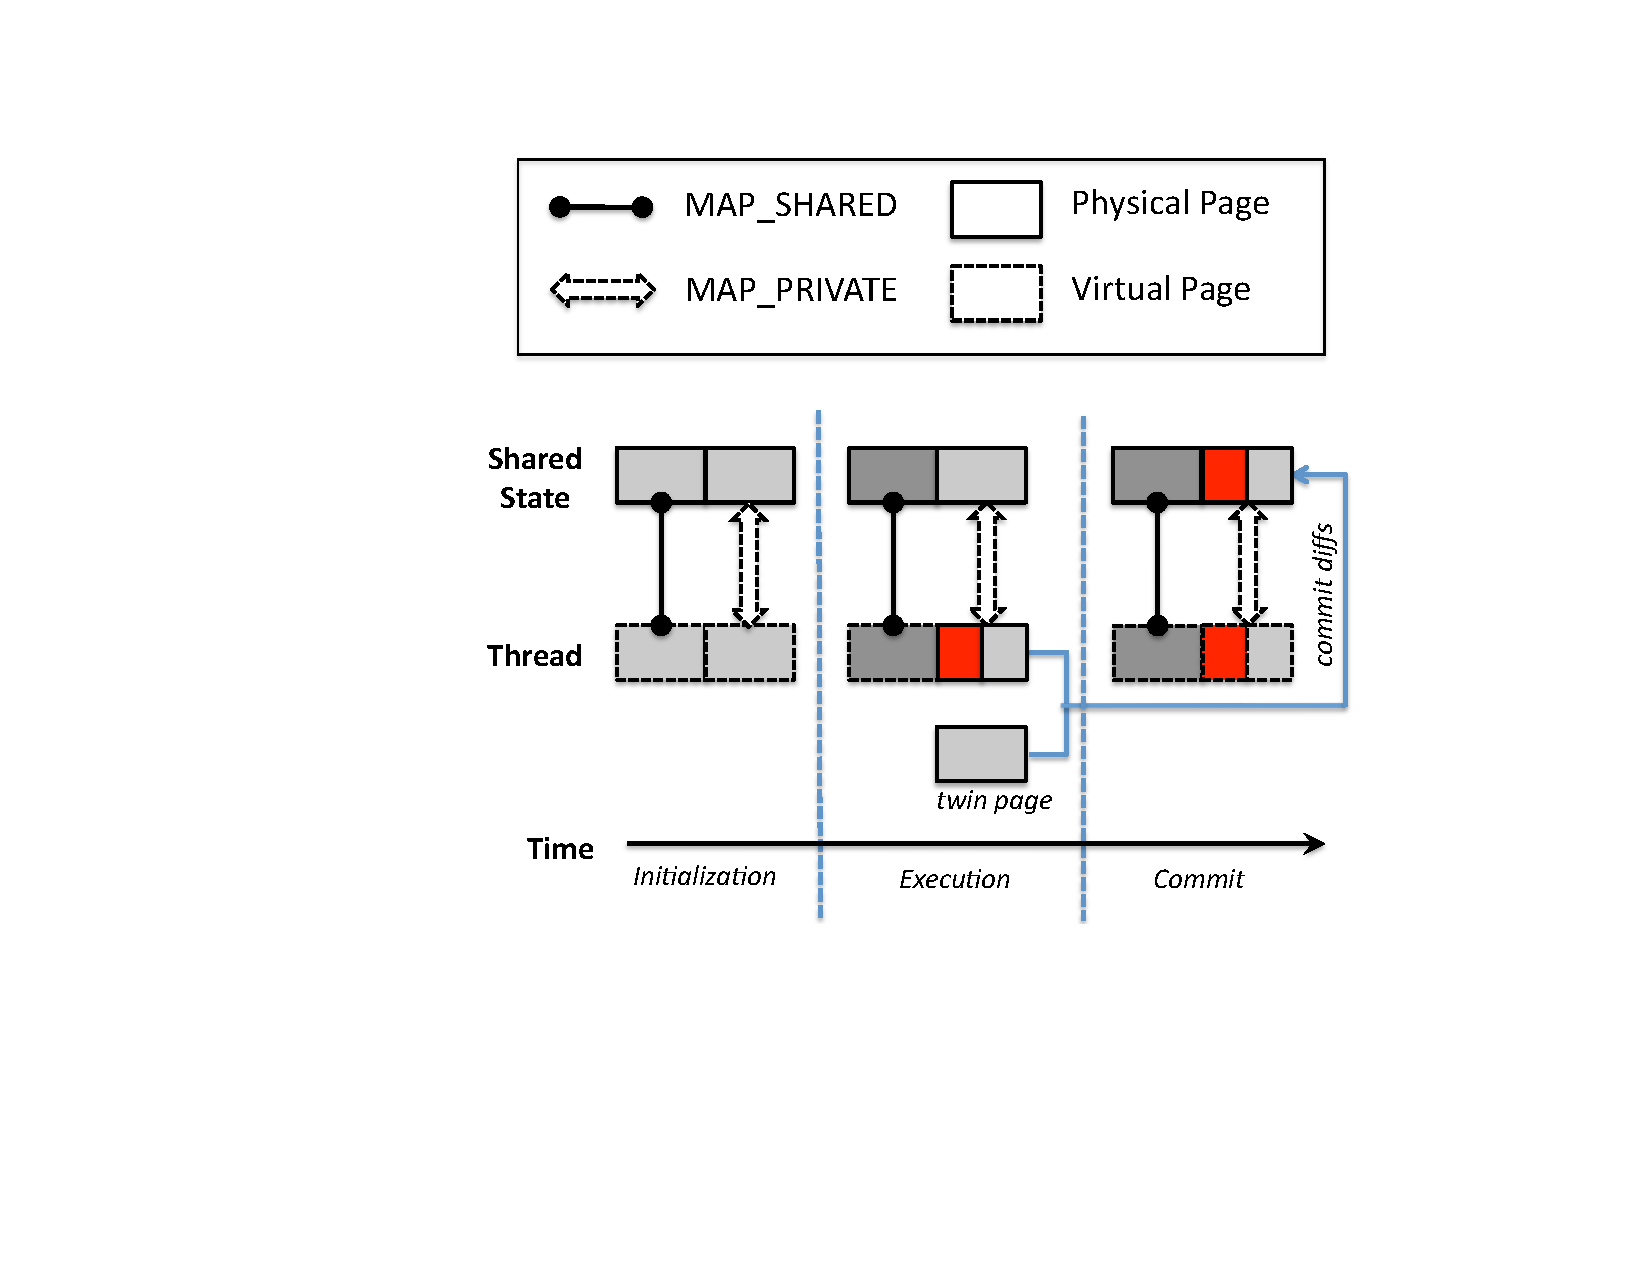
\includegraphics[width=3.5in]{sheriff/figure/sheriffframework.pdf}
\caption{\sheriff{} execution inside a transaction
\label{fig:sheriffoverview}}
\end{figure} 

\sheriff{} intercepts all threads synchronizations and breaks the whole execution of each thread to 
multiple transactions based on synchronization boundaries: 
those sections of each thread between synchronization points and critical sections
are considered as separate transactions.
Those synchronizations includes locks, conditional variables, barriers and 
various types of thread exits and signals.
\sheriff{} wraps all synchronizations in a similar way as the following example:
a call to \texttt{pthread\_mutex\_lock} first ends the current transaction; 
\sheriff{} calls \pthreads{}'s process-shared \texttt{pthread\_mutex\_lock};  
\sheriff{} starts a new transaction after the lock is acquired and ends at the next 
possible synchronization operation, one of \texttt{pthread\_mutex\_unlock}, 
\texttt{pthread\_cond\_wait} or \texttt{pthread\_cond\_signal} calls.
Figure~\ref{fig:sheriffoverview} shows the execution in a single transaction. 

\textbf{Transaction Begin:}
In the beginning of every transaction, \sheriff{} write-protects all private pages in order to
capture writes on those pages by handling \texttt{SEGV} protection faults.  

\textbf{Execution:} In the execution phase, reads on non-faulted pages in this transaction 
are performed on the shared mapping directly. The first write on
a protected page invokes a page fault. By handling this fault,  
\sheriff{} records those faulted pages, creates twin pages 
and unprotects them so that future accesses can run at full speed.  

\textbf{Transaction End:} At the end of each transaction, \sheriff{} 
commits local changes of each process to the shared mapping by using twinning-and-diffing mechanism, 
reclaims those temporary pages and
recovers the permissions for those pages written in this transaction. 
   
Through this, \sheriff{} achieves the same semantics as 
that of \pthreads{} for programs without races
and \texttt{ad hoc} synchronizations (see~\cite{ad-hoc-considered-harmful} for the definition).
% shared variables accesses should be synchronized correctly.

%\subsection{Difference with \grace{}}
%\sheriff{} extends the processes-as-threads concept introduced by \grace{} but
%with different semantics, generality and goals. 

%\grace{} is designed to tolerate concurrency errors by imposing a sequential semantics. 
%\grace{} only supports fork-join programs without inter-thread communications (e.g. conditional 
%variables and barriers), relying on a rollback mechnism to ensure  
%sequential semantics and determinism. 

%\sheriff{} supports general multithreaded programs without any annotations or changes of
%programs. \sheriff{} does not prevent the usage of inter-thread synchronizations at all. 
%Since there is no rollback mechanism and protections on read operations, 
%\sheriff{} generally runs much
%faster than \grace{}, without any guarantee of determinism.

\section{False Sharing Detection}
% How to find out the "false sharing problem" ? We are trying to get those callsite information. 
% False sharing problem means that two threads are accessing different words in the same cache line
% and one of them is a read operations. 
\SheriffDetect{} is a tool to detect false sharings of multithreaded programs, built on
top of the \sheriff{} framework. 
As we described in Section~\ref{falsesharing}, false sharing can greately slow down the program 
when there are a lot of interleaved writes from different threads on the same cache line.
\SheriffDetect{} captures all cache lines with interleaved writes and 
ranks the seriousness by the frequency 
of interleaved writes: cache lines with more interleaved writes are considered to have more 
performance impact on the programs.  

Relying on ``per-thread-isolation'' and ``per-thread-protection'' mechanisms to track written pages, 
combining with twinning-and-diffing mechanism (explained in Section \ref{sec:twinning-and-diffing}),
\SheriffDetect{} can find out per-process modifications in the end of each transaction.
However, for a long transaction, checking in the end of each transaction is not enough because it
may loose multiple modifications inside each transaction.
So \SheriffDetect{} periodically samples the modifications for those long transactions. 

Based on this, \SheriffDetect{} utilizes the following mechanisms to report false 
sharings precisely and accurately. 

\begin{itemize}

\item  
In order to precisely report origins of false sharing objects, \SheriffDetect{} keeps callsite 
information for each heap object and reports the source code level information about 
each object. 

\item
%In order to avoid reporting true sharing problems, 
\SheriffDetect{} tracks modifiers and numbers of modifications for each word so that 
\SheriffDetect{} can only reports a cache line with actual false sharing problems.  
In the meanwhile, numbers of modifications on each word helps to identify 
actual causes since there are multiple fields or multiple objects 
in the same cache line.  

\item
To avoid the pseudo false sharing problems caused by memory re-usages, 
\SheriffDetect{} intercepts the memory allocations and deallocations functions 
and handles them correspondingly. \SheriffDetect{} is the first work to observe and deal 
with problems caused by memory re-usage.
%When an objectXXXXXXXXXXX 

\end{itemize}  

In conclusion, \SheriffDetect{} is the first practical tool, 
only introducing 21\% performance overhead,to locate false sharing
problems precisely and accurately.
Now the tool is used by \texttt{SAS} and \texttt{Intel} company 
to detect false sharings of their actual products. 
However, it is impossible for \SheriffDetect{}
to identify read operations with reasonable overhead,  
so \SheriffDetect{} can not be used to detect read-write false 
sharing problems: one writer and multiple 
readers in the same cache line.

% Problem of this approach, we can't detect the single-writer cases. 

\section{False Sharing Prevention}
% What is the basic idea of \sheriffProtect{}.

We observes a fact from \SheriffDetect{}: isolating executions of 
different threads actually improves performance for those programs with serious false sharings.
Here, different processes actually access different physical pages after the first 
write inside a transaction, the ping-pong effect of loading-and-invalidating is actually prevented by doing this. 

Based on this observation, we developed \SheriffProtect{} to tolerate false sharings
of multithreaded programs utilizing the following mechanisms. 

\begin{itemize}
\item
\SheriffProtect{} only makes pages private when it is beneficial to do this. 
A private page can tolerate false sharings while introducing 
different types of overhead inside a transaction: 
protection overhead in the beginning, 
page fault and commit overhead for those written pages and the overhead to reclaim temporary pages 
in the end.
When a page does not have false sharings, 
the overhead can slow down the execution and should be avoided as much as possible.
In out implementation, \SheriffProtect{} only prevents the false sharings
on small objects (those less than 1024 bytes in size) and all large objects 
are mapped shared without any protection. 
 

\item
Short transactions does not give any performance benefit because the overhead we mentioned above
can be larger than the benefit by preventing false sharings.
\SheriffProtect{} employs a simple adaptive mechanism to avoid this problem: 
we only protect the memory when a transaction is longer than a specific threshold. 
However, this approach also means that we can not tolerate false sharings for 
programs with intensive synchronizations. 
For a program with intensive synchronizations, 
it is better to rely on
\SheriffDetect{} to find false sharings and fix it manually.  

\end{itemize}
 

% What is the result of \sheriff{}.


\chapter{\Predator{}: Predictive False Sharing Detction}
This chapter presents \Predator{}, which improves the detection of false sharing. \SheriffDetect{} reports false sharing accurately and precisely with only $20\%$ performance overhead. However, it can only detect write-write false sharing for those programs using \pthreads{} library. It can also break programs that communicate across different threads with stack variables or self-defined synchronizations. These shortcomings greatly limit \Sheriff{}'s usage on real-world applications.  

In contrast to \SheriffDetect{}, \Predator{} detects all types of false sharing and has no limitations on applications. \Predator{} has been utilized to find actual false sharing in real applications, including \texttt{MySQL} and the \texttt{Boost} library.

In addition, \SheriffDetect{} and other systems share one key limitation: they can only report \emph{observed} cases of false sharing. As Nanavati et al.\ point out, false sharing is sensitive to where objects are placed in cache lines and so can be affected by a wide range of factors~\cite{OSdetection}. For example, using the gcc compiler \emph{accidentally} eliminates false sharing in the Phoenix linear\_regression benchmark at certain optimization levels, while LLVM does not do so at any optimization level.  A slightly different memory allocation sequence (or different memory allocator) can reveal or hide
false sharing, depending on where objects end up in memory; using a different hardware platform with different addressing or cache line sizes can have the same effect. All of this means that existing tools cannot root out potentially devastating cases of false sharing that could arise with different inputs, in different execution environments, and on different hardware platforms.

\Predator{} is the first system that can \emph{predict} potential false sharing that does not manifest in an execution but may appear and greatly degrade the performance of programs in a slightly different
environment. Predictive false sharing generalizes from a single execution to identify potential false sharing instances that are within one cache line of each other, which could be exposed by slight changes in object placement and alignment. It also can predict false sharing in hardware platforms with larger cache line sizes by tracking accesses within \emph{virtual cache lines} that span multiple physical lines. Predictive false sharing detection thus overcomes a key limitation of previous detection tools.

\section{False Sharing Detection}
\label{sec:detection}

We first describe \Predator{}'s false sharing detection mechanism, which consists of both compiler and runtime system
components. Section~\ref{sec:prediction} then explains how \Predator{} predicts potential false sharing based on a single execution.

\subsection{Overview}
\label{sec:overview}
False sharing only occurs when two threads
simultaneously access independent data in the same cache line.
In the remainder of this paper, we assume for the purposes of exposition that each thread runs on a 
distinct core with its own private cache.

Given this assumption, we observe that 
if a thread writes a cache line after other threads have 
accessed the same cache line, this write operation most likely causes at least a cache invalidation. Drawing from this \textbf{basic observation}, \Predator{} tracks cache invalidations of all cache lines and ranks the severity of performance degradation of any detected false sharing problems according to the number of cache invalidations. 
% by keeping track of accesses from different threads. 
 
In order to track cache invalidations, \Predator{} relies on the compiler instrumentation to track memory accesses of applications. The design tradeoff of choosing compiler instrumentation has been discussed in Section~\ref{sec:instrumentationtradeoff}. A compiler can easily identify read or write accesses. However, a compiler does not know how and when those instructions are being executed, since that depends on a specific execution, input, and runtime environment.

Therefore, \Predator{} combines a runtime system with compiler
instrumentation to track cache invalidations: the compiler
instruments memory accesses so the runtime system is notified when an access is executed (see Section~\ref{sec:compiler}), and the runtime system is responsible for collecting and analyzing actual memory accesses to detect and report false sharing (see Section~\ref{sec:runtime}).

\subsection{Compiler Instrumentation}
\label{sec:compiler}

\Predator{} relies on LLVM to perform instrumentation at the intermediate representation level~\cite{llvm}.
It traverses all functions one by one and searches for memory accesses to global and heap variables.  For each memory access, \Predator{} instruments a function call to invoke the runtime system with the memory access address and access type. \Predator{} currently omits accesses to stack variables by default because stack variables are normally used for thread local storage and therefore do not normally introduce false sharing. However, instrumentation on stack variables
can always be turned on when necessary.

The instrumentation pass is placed at the very end of the LLVM
optimization passes so that only those memory accesses surviving all previous LLVM optimization passes are instrumented.  This technique is similar to the one used by AddressSanitizer~\cite{AddressSanitizer}.

\subsection{Runtime System}
\label{sec:runtime}

\Predator{}'s runtime system collects every memory access by handling those functions calls inserted during the compiler instrumentation phase. It analyzes possible cache invalidations based on the basic observation discussed in Section~\ref{sec:overview}. Finally, \Predator{} precisely reports any performance-degrading false sharing problems it finds.  For global variables involved in false sharing, \Predator{} reports their name, address and size; for heap
objects, \Predator{} reports the callsite stack for their allocations, their address and size. In addition, \Predator{} provides word granularity access information for those cache lines involved in false sharing, including which threads accessed which words.  This information can further help users diagnose and fix false sharing instances.

\subsubsection{Tracking Cache Invalidations}
\Predator{} only reports those global variables or heap objects on cache lines with a large number of cache invalidations. It is critical to track cache invalidations effectively so that \Predator{} delivers accurate reports.
\Predator{} achieves this goal by maintaining a two entry cache history table for each cache line.  In this table,
each entry has two fields: the thread ID and access type (read or write). The thread ID is used to identify the origin of each access. As stated earlier, only accesses from different threads can cause cache invalidations.

\begin{comment}
\begin{table}
\centering
  \begin{tabular}{ l | r }
    \hline
    {Thread ID} & {Type of Access} \\ \hline
    \hline
     &   \\ \hline
     &   \\ \hline
  \end{tabular}
  \caption{Two-entries-cache-history table for every cache line. \label{table:cachehistory}}
\end{table} 
\end{comment}

For every new access to a cache line $L$, \Predator{} checks $L$'s history table $T$ to decide whether there is a cache invalidation based on the following rules.  Note that table $T$ only has two statuses: full and not full.  There is no ``empty'' status since every cache invalidation should replace this table with the current write access.

\begin{itemize}
\item
  For a read access $R$, 
  \begin{itemize}
    \item
      If $T$ is full, there is no need to record this read access.
    \item
      If $T$ is not full and another existing entry has a different thread
      ID, then \Predator{} records this $R$ and its thread by adding a new entry to the table. 
  \end{itemize}
\item
  For a write access $W$, 
  \begin{itemize}
    \item
      If $T$ is full, then $W$ can cause a cache invalidation since at least one of two existing entries has a different thread ID.
      After recording this invalidation, \Predator{} updates the
      existing entry with $W$ and its thread.
    \item
      If $T$ is not full,
      \Predator{} checks whether $W$ and the existing entry has the same thread ID. If
      so, $W$ cannot cause a cache invalidation, so \Predator{} updates the existing
      entry with $W$. Otherwise, \Predator{} identifies an invalidation on this line caused by $W$. 
      After recording this invalidation information, \Predator{} updates the
      existing entry with $W$ and its thread.
  \end{itemize}
\end{itemize}

\subsubsection{Reporting False Sharing}

After the cache lines with a large number of cache invalidations are detected,
\Predator{} needs further analysis to differentiate actual false sharing from true sharing. 
True sharing, e.g., multiple threads updating the same counter in a cache line, can also cause a large number of cache invalidations.

In order to report false sharing precisely and accurately,  
\Predator{} employs the following mechanisms. 

\begin{itemize}
\item

\Predator{} keeps track of access information for each word on those cache lines involved in false sharing: how many reads or writes to each word by which thread.  When a word is accessed by multiple threads, we mark the origin of this word as a shared access and do not track threads for further accesses to it. This information lets \Predator{} accurately distinguish false sharing from true sharing in the reporting phase.  It also helps diagnose where
actual false sharing occurs when there are multiple fields or multiple
objects in the same cache line, as this can greatly reduce the manual
effort required to fix the false sharing problems.

\item
In order to precisely report the origins of heap objects with false
sharing problems, \Predator{} maintains callsite information for each heap
object and reports source code level information for each heap
object. To obtain callsite information, \Predator{} intercepts all memory allocations and de-allocations, and relies
on the \texttt{backtrace()} function in the \texttt{glibc} library to obtain the whole callsite stack.
\Predator{} also avoids pseudo false sharing (false positives) caused by memory reuses because it updates recording information at memory de-allocations for those objects without false sharing problems; heap objects involved in false 
sharing are never reused.


\item
For every access, \Predator{} needs to lookup the corresponding cache line's metadata 
in order to store detailed information or update access counters. Because this operation is so frequent,
 lookups need to be very efficient.
Like 
AddressSanitizer~\cite{AddressSanitizer} and other systems~\cite{qinzhao,Valgrind},
\Predator{} uses a shadow memory mechanism to store metadata for every piece of application data. 
Thus, \Predator{} can compute and locate corresponding metadata directly via address arithmetic.

\item
In order to support shadow memory, \Predator{} uses a predefined starting address and fixed size for its heap.  It also contains a custom memory allocator, which is built with Heap Layers~\cite{heaplayers} using a ``per-thread-heap'' mechanism similar to that used by Hoard~\cite{Hoard}.  In this allocator, memory allocations from different threads never occupy the same physical cache line, which automatically avoids false sharing among different objects.  However, using this custom memory allocator implies that false sharing caused by a memory allocator cannot be detected by \Predator{}. The way to solve any such false sharing problem is to use a better allocator, since allocators like Hoard already avoid this kind of false sharing.

\end{itemize} 
 
\subsection{Optimizations}
\label{optimization}
Tracking every memory access can be extremely expensive, thus 
\Predator{} utilizes the following mechanisms to further reduce overhead.

\subsubsection{Threshold-Based Tracking Mechanism}
\label{sec:thresholdtracking}
\Predator{} aims to detect false sharing that significantly degrades performance. Since cache invalidations are the root cause of performance degradation and only writes 
can possibly introduce cache invalidations, 
cache lines with a small number of writes are never a significant performance bottleneck.
For this reason, \Predator{} only tracks cache invalidations
once the number of writes to a cache line crosses a
pre-defined threshold, which we refer to as the {\it Tracking-Threshold}. 
Before this threshold is reached, \Predator{} only tracks the number of writes on a cache line 
while skipping tracking for reads.
This mechanism reduces performance and memory overhead
at the same time.

In the current implementation, \Predator{} maintains two arrays in shadow memory: 
{\it CacheWrites} is used to track the number of memory writes on every cache line, and
{\it CacheTracking} tracks detailed information 
for each cache line once the number of writes on a cache line exceeds
the {\it Tracking-Threshold}. 
If the threshold is not reached, there is no need to check the corresponding {\it CacheTracking}. 
Figure~\ref{fig:algorithm} illustrates the detailed mechanism.

\begin{figure}[!t]
\begin{lstlisting}
void HandleAccess(unsigned long addr, bool isWrite) {
 unsigned long cacheIndex=addr>>CACHELINE_SIZE_SHIFTS;
 cachetrack *track=NULL;

 if(CacheWrites[cacheIndex]<TRACKING_THRESHOLD) {
  if(isWrite) {
   if(ATOMIC_INCR(&CacheWrites[cacheIndex]) 
      ==TRACKING_THRESHOLD-1) {
    track=allocCacheTrack();
    ATOMIC_CAS(&CacheTracking[cacheIndex],0,track));
   }
  } 
 }
 else {
  track=CacheTracking[index]);
  if(track){
   // Track cache invalidations and detailed accesses
   track->handleAccess(addr, isWrite);
  }
 }
}
\end{lstlisting}
\caption{Pseudo-code to handle an access.\label{fig:algorithm}}
\end{figure}

To avoid expensive lock operations, \Predator{} uses atomic instruction to increment 
the {\it CacheWrites} counter for each cache line. 
When the number of writes of a cache line reaches the predefined threshold,
it allocates space to track detailed cache invalidations and word accesses.
\Predator{} also 
uses an atomic compare-and-swap to set the cache tracking address for this cache line in
the shadow mapping.
After {\it CacheWrites} on a cache line reaches the {\it Tracking-Threshold}, 
all read and write accesses on this cache line are tracked.
%Cache invalidations are also computed based on cache line history table of corresponding
%cache line, shown in Table~\ref{table:cachehistory}. 


\subsubsection{Selective Compiler Instrumentation}
\label{sec:selectinstrumentation}

\Predator{} relies on instrumentation to provide memory access information to the runtime system 
and detects false sharing based on the sequences of memory accesses on every cache line. 
The performance overhead of a specific program is always proportional to 
the degree of instrumentation: more 
instrumentation means more performance overhead. 
Thus, \Predator{} provides a flexible framework to instrument programs 
depending on the performance requirements of the user.

Currently, \Predator{} only adds instrumentation once for each type of memory access on each address 
to the same basic block. 
This selective instrumentation does not normally affect the effectiveness of detection. 
Because \Predator{} aims to detect false sharing cases with a large number of cache invalidations,
less tracking of accesses inside a basic block can induce fewer cache invalidations 
but it does not affect the overall behavior of cache invalidations. 

% detection will not cause performance problem. 
To improve performance further,
\Predator{} can be easily extended to support more flexible instrumentation as follows:
\begin{itemize}
\item
\Predator{} could selectively instrument both reads and writes or only writes.
Instrumenting only writes reduces overhead while detecting write-write false sharing, 
as \Sheriff{} does. 
\item
\Predator{} can be set to instrument or skip specific code or data. 
For example, the user could provide a black-list so that given modules,
functions or variables are not instrumented. 
Conversely, the user could provide a white-list so that only specified functions or variables are instrumented. 
\end{itemize}

\subsubsection{Sampling Mechanism}
\label{sec:sample}
As described in Section~\ref{sec:thresholdtracking}, when the number of
writes on a cache line is larger than {\it Tracking-Threshold}, every
access must be tracked to store details such as word access
information, update access counter, and the cache access history table
of this cache line.  When a cache line is involved in false or true
sharing, updating those counters can exacerbate the impact of sharing
on performance: not only is there an invalidation on an application
cache line, but there is also at least another cache invalidation
caused by updating the metadata of the corresponding cache lines.

To further reduce performance overhead, \Predator{} only samples the first specified
number of accesses of each sampling interval for those problematic cache lines. 
%Note that we originally keep a global counter for all accesses and uses the number of 
%all accesses to compuate sample intervals. However, this creates 
%extereme performance overhead caused by cache invalidations of updating the same counter
%for all accesses. 
Currently, \Predator{} maintains an access counter for each cache line
and only tracks the first $10,000$ accesses out of every 1 million
accesses on a cache line (a 1\% sampling rate).



\section{False Sharing Prediction}
% Why prediction is important?
\label{sec:prediction}
This section further motivates predictive false sharing and explains how to support it in the runtime system.  

\subsection{Overview}
%\begin{figure*}[!htb]
\label{sec:predictoverview}

\begin{figure}[!t]
\begin{center}
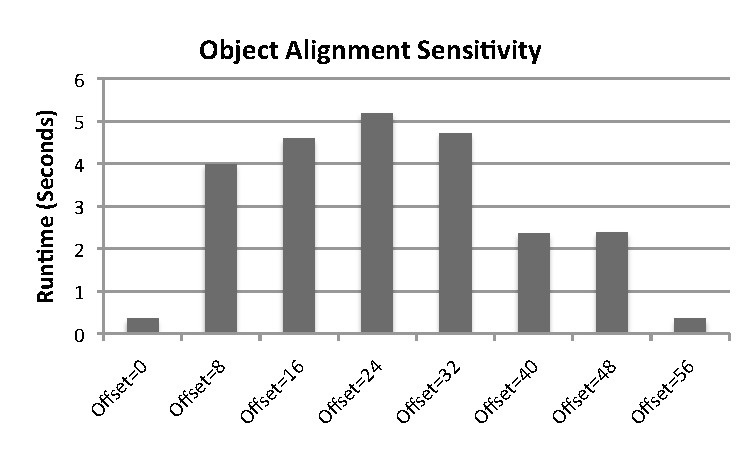
\includegraphics[width=3.3in]{predator/figure/perfsensitive}
\end{center}
\caption{
Performance of the linear\_regression benchmark from the Phoenix benchmark suite.
Performance is highly sensitive to the offset of the starting address of the (potentially) falsely-shared object 
and the start of cache line. 
\label{fig:perfsensitive}}
\end{figure}

The appearance of false sharing depends on 
the alignment between objects and corresponding cache lines.
A real example, linear\_regression, is shown in Figure~\ref{fig:perfsensitive}.
For this benchmark,
when the offset of the starting address between the potentially falsely-shared object and corresponding cache lines 
is $0$ or $56$ bytes, 
there is no false sharing. 
When the offset is $24$ bytes, we see the most severe performance effect caused 
by false sharing. 
The performance difference between these two scenarios can be as large as $15\times$. 
Existing detection tools can only report observed false sharing.
For this case, they may miss a very severe false sharing problem that could occur in the wild if the offset of the starting 
address was $0$ bytes or $56$ bytes in their test environment.
\Predator{} overcomes this shortcoming by accurately predicting potential false sharing.

\begin{figure*}
\begin{center} 
\subfigure[No false sharing]{%
   \label{fig:nofs}
   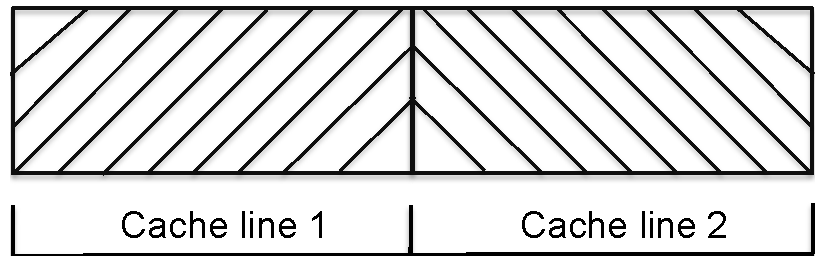
\includegraphics[width=0.24\textwidth]{predator/figure/Potential1}
}%
\hspace{30pt}
\subfigure[False sharing with larger cache size]{%
   \label{fig:fslarger}
   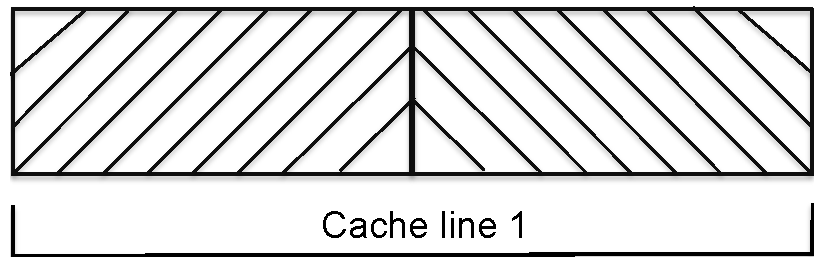
\includegraphics[width=0.24\textwidth]{predator/figure/Potential2}
}%
\hspace{30pt}
\subfigure[False sharing with different alignment]{%
   \label{fig:fsnoalignment}
   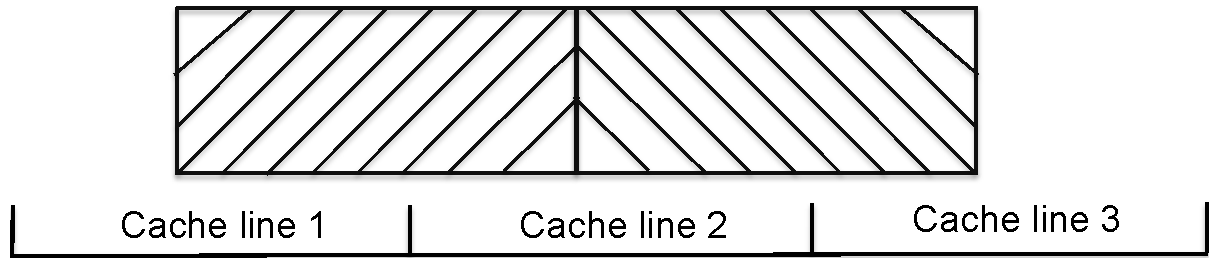
\includegraphics[width=0.36\textwidth]{predator/figure/Potential3}
}%
\end{center}
%\includegraphics{fig/potential.pdf}
\caption{False sharing under different environments.}
\label{fig:potentialfalsesharing}
\end{figure*}

\Predator{} predicts {\it potential false sharing}, the type of
false sharing that does not 
manifest in the current execution but may appear and greatly affect programs' performance
in a slightly different environment.

Figure~\ref{fig:potentialfalsesharing} shows a simplified example why occurrences of false sharing 
can change in different situations.
In this figure, two rectangles with different patterns
represents two portions of the same object, updated by different threads. 
In Figure~\ref{fig:nofs}), there is no false sharing when thread T1 only updates 
``cache line 1'' and T2 only updates ``cache line 2''.
However, false sharing appears in one of the following cases, even with the same
access pattern. 

\begin{itemize}
\item
Doubling cache line size (Figure~\ref{fig:fslarger}). When the size of a
cache line doubles,
both T1 and T2 access the same cache line and false sharing occurs in this case.

\item
Different starting address of an object(Figure~\ref{fig:fsnoalignment}). 
When the starting address of this object is not aligned with the starting address of 
the first cache line, 
then T1 and T2 can update the second cache line simultaneously, 
causing false sharing. 
%When some dynamic property changes the starting address of this object so that it 
%is not aligned with the starting address of the first cache line, 
\end{itemize} 

\Predator{} predicts whether programs can have potential false sharing  
in either of these two cases, where they can be caused by different dynamic properties 
discussed in Section~\ref{sec:intro}.
All dynamic properties, except the change of cache line size,
can lead to different starting address of an object. 
Thus, predicting false sharing in these two cases actually 
explores many possibilities caused by all dynamic properties.

\subsection{Basic Prediction Workflow}
\label{sec:predictionmechanism} 

%Similar to the detection part, 
\Predator{} focuses exclusively on potential false sharing that can 
cause performance problems.
The implementation is based on
two key observations. First, only accesses to 
adjacent cache lines can form potential false sharing, 
i.e., introducing cache invalidations when cache line size
or an object's starting address changes.
Second, only when false sharing introduces a large number of cache invalidations
can it degrade performance.

Based on these two observations, \Predator{} develops 
the following workflow to capture potential false sharing.
Those detection optimizations listed in Section~\ref{optimization} can also be applied
to prediction part. We do not repeat these optimizations in this section.

\begin{enumerate}
\item
Track the number of writes on different cache lines. 

\item
When the number of writes to a cache line $L$ reaches {\it Tracking-Threshold},
track the detailed read and write accesses for every word on both cache line $L$ 
and its adjacent cache lines. 

\item
When the number of writes to a cache line $L$ reaches a second threshold (called as
{\it Predicting-Threshold}), 
identify whether there exists false sharing in $L$ and its adjacent 
cache lines by analyzing word accesses information collected in Step 2. 
Section ~\ref{sec:evaluatingfs} describes the evaluation method.

\item
If a potential false sharing is found, continue to track cache line invalidations to confirm it. Section~\ref{sec:tracking} discusses the details.
Otherwise, go back to Step 2 to track more detailed accesses.
 
\end{enumerate}

\subsection{Searching for Potential False Sharing}
\label{sec:evaluatingfs}
To describe potential false sharing in two different cases, we first 
introduce the concept of a virtual cache line.  A virtual cache line
is a contiguous memory range that spans one or more physical cache 
lines.  In the case of double cache line size, a virtual line is
composed of two original contiguous cache lines and the first cache
line has an even index number.  Thus, only cache lines $2*i$ and
$2*i+1$ can form a virtual line.  In the case of different starting
addresses, a virtual line can have the same size as physical lines,
but can be positioned arbitrarily: unlike actual cache lines, the
starting address of a virtual cache line does not need to be multiple
of the cache line size.  For instance, a 64-byte long virtual line can
consist of the range $[0,64)$ bytes or $[8,72)$ bytes.

To search for potential false sharing problems, 
\Predator{} searches for a hot access pair on $L$ and its adjacent cache lines 
by analyzing the detailed word access information collected in Step 2. 
A hot access in a cache line refers to the word whose number of read or write accesses 
is larger than the average number of accesses to each word of cache line $L$.
For every hot access $X$ in cache line $L$, \Predator{} searches another
hot access $Y$ in $L$'s previous cache line or next cache line satisfying
the following conditions: 

\begin{itemize}
\item
$X$ and $Y$ reside on the same virtual line. 

\item
One of $X$ and $Y$ is a write access.

\item 
$X$ and $Y$ are issued by different threads.

\end{itemize}

% why it finds a pair of $X$ and $Y$ == a potential false sharing 
Whenever it finds such a pair $X$ and $Y$, 
\Predator{} identifies potential performance-degrading false sharing whenever
 the number of cache invalidations caused by $X$ and $Y$, at a possible virtual line, 
is larger than the average number of accesses on each word of $L$. 
This approach is based on a similar observation as in detection:
\emph{if a thread writes a virtual line after other threads 
have accessed the same virtual line, this write operation most likely causes at least one cache 
invalidation}. 
Before tracking detailed memory accesses on a virtual line, it is impossible to know exactly how many cache invalidations happen on a virtual line. Thus, \Predator{} conservatively assumes that accesses from different threads occurs interleavedly.
This approach ensures that \Predator{} does not miss any potential false sharing as well as 
not reporting false positives. 

%According to above observation and assumption, 
%a pair of hot accesses, $X$ and $Y$, if accesses are issued in an interleaving 
%way, can generate the number of cache invalidations equaling to 
%the smaller number of accesses of $X$ and $Y$.
%Thus a false sharing problem is to be identified by \Predator{}.
  
After identifying possible false sharing, \Predator{} goes to Step 4 to 
verify whether this is an actual false sharing problem.

\subsection{Verifying Potential False Sharing}
\label{sec:tracking}

\Predator{} verifies potential false sharing by tracking 
cache invalidations on a problematic virtual line.
%covering a pair of hot accesses found
%in Step 3.

For potential false sharing caused by double cache line size, as described in
Section~\ref{sec:evaluatingfs}, a virtual line is always composed of 
cache line with index $2*i$ and $2*i+1$. 
\Predator{} tracks cache invalidations
on the virtual line on which false sharing has been discovered.

However, for the case of a change in starting address,
two hot accesses with distance less than cache line size 
can form multiple virtual lines. 
There is thus an additional step to determine which virtual line to be tracked.
Although the virtual line to be chosen here is never a real cache line of actual hardware
because of unaligned addresses,
we utilize this virtual line to simulate the effect of changing the 
starting addresses of objects.


\begin{figure}
\begin{center} 
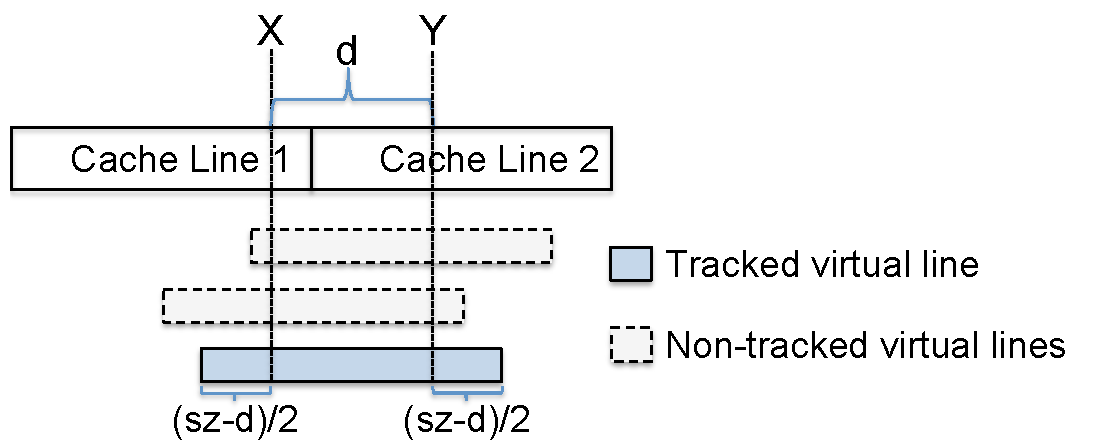
\includegraphics[width=3.3in]{predator/figure/trackpotential}
\end{center}
\caption{Determining a virtual line with size $sz$ according to hot accesses.}
\label{fig:trackpotential}
\end{figure}

Given two words with the hot accesses shown in Figure~\ref{fig:trackpotential}, 
\Predator{} leaves the same space before $X$ and after $Y$ in determining a virtual line. 
That is, the virtual line starting 
at location $X-((sz-d)/2)$ and ending at $Y+((sz-d)/2)$ is tracked. 
This choice allows tracking of more possible cache invalidations caused by
adjacent accesses of $X$ and $Y$. 
Since adjusting the starting address of a virtual line has the same effect of
adjusting the starting address of an object in detecting false sharing,
all cache lines related to the same object must be adjusted at the same time.
\Predator{} then tracks cache invalidations based on these adjusted virtual lines.



\section{Evaluation}
\begin{figure*}[htb]
{\centering
\tiny
\subfigure{\lstinputlisting[numbers=none,frame=none,boxpos=t]{predator/figure/linearregression.report}}
\caption{An example report by \Predator{} indicating false sharing in the linear\_regression benchmark.
\label{fig:lrreport}}
}
\end{figure*}



\label{sec:evaluation}

This section answers the following questions:
\begin{itemize}
\item
  How effective is \Predator{} at detecting and predicting false sharing?

\item
  What is \Predator{}'s overhead, in terms of execution time and memory ?

\item
  How sensitive is \Predator{} to different sampling rates?
 
\end{itemize}

\paragraph{Experimental Platform.} All evaluations are performed on a quiescent Intel Core 2 dual-processor system equipped with 
16GB RAM. Each processor is a 4-core 64-bit Intel Xeon running at 2.33 GHz, with a 4MB shared L2 cache and 32KB private L1 cache. The underlying operating system is an unmodified CentOS 5.5, running with Linux kernel version 2.6.18-194.17.1.el5. The glibc version is 2.5. 

\paragraph{Evaluated Applications.}
This paper evaluates two popular benchmark suites,
Phoenix (with large input) ~\cite{phoenix-hpca} and PARSEC (with simlarge input) ~\cite{parsec}. Even with unmodified LLVM-3.2, Facesim cannot be compiled successfully (having complaints on an undefined template) and Canneal aborts unexpectedly. Thus, these two benchmarks are excluded.
We also evaluate \Predator{} on six real applications, including MySQL, Boost, Memcached, aget, pbzip2 and pfscan.



\subsection{Detection and Prediction Effectiveness}
\label{sec:effective}

For every false sharing problem, \Predator{} reports source code information and detailed memory access information in order to help users fix those problems. Figure~\ref{fig:lrreport} shows an example for the linear\_regression benchmark. This report shows that the heap object starting with $0x40000038$ potentially causes a large number of cache invalidations. The call stack of allocation is provided to help locate culprits. In addition, \Predator{} also reports word-level access information of this object, which helps to identify where and how false sharing occurs. From that, we can know that it is a latent false sharing problem predicted by \Predator{}, since different threads are accessing different cache lines. 

\subsubsection{Benchmarks}
\label{sec:benchmarks}

\begin{table*}[!t]
{\centering\begin{tabular}{l|r|r|r|r|r}\hline
{\bf \small Benchmark} & {\bf \small Source Code} & {\bf \small New} & {\bf \small Without Prediction} &{\bf \small With Prediction} & {\bf \small Improvement} \\
\hline
\small \textbf{histogram} & {\small histogram-pthread.c:213} & \cmark{} &\cmark{} & \cmark{} & 46.22\%\\
\small \textbf{linear\_regression} & {\small linear\_regression-pthread.c:133} & & & \cmark{} & 1206.93\% \\
\small \textbf{reverse\_index} & {\small reverseindex-pthread.c:511} & & \cmark{} & \cmark{} & 0.09\%\\
\small \textbf{word\_count} & {\small word\_count-pthread.c:136} & & \cmark{} & \cmark{} & 0.14\%\\
\hline
\small \textbf{streamcluster} & {\small streamcluster.cpp:985} &  & \cmark{} & \cmark{} &7.52\% \\
\small \textbf{streamcluster} & {\small streamcluster.cpp:1907} & \cmark{} & \cmark{} & \cmark{} & 4.77\%\\
\hline
\end{tabular}
\caption{False sharing problems in the Phoenix and PARSEC benchmark suites. \label{table:detection}}
}
\end{table*}

Table~\ref{table:detection} provides detection results of two benchmark suites, Phoenix and PARSEC
The first column lists those programs with false sharing problems.  The second column shows precisely where the problem is. Because all discovered false sharing occurs inside heap objects, we show callsite source code information here.  The third column, ``New'', marks whether this false sharing was newly discovered by \Predator{}.  A checkmark in the following two columns indicates whether the false sharing was identified without
prediction and/or with prediction.  The final column, ``Improvement'', shows the performance improvement after fixing false sharing.
%The number is based on the average runtime of $10$ runs. 

As shown in the table, \Predator{} reveals two unknown false sharing problems. It is the first tool to detect the false sharing problems in histogram and in line $1908$ of streamcluster. 
In histogram, multiple threads simultaneously modify different locations of the same heap object, thread\_arg\_t. 
Padding this data structure fixes the false sharing problem and improves the performance by around 46\%. In streamcluster, multiple threads are simultaneously accessing and updating the same \texttt{bool} array, switch\_membership. Simply changing all elements of this array to a long type reduces the false sharing and improves the performance by about 4.7\%.

%, although it is not a complete fix of false sharing. 
%None of these two false sharing problems has been reported by previous tools.
Other false sharing problems were discovered by previous work~\cite{sheriff}. We do not see significant performance improvement for reverse\_index and word\_count benchmarks. They are reported here because the number of cache invalidations in these two programs reaches our predefined threshold.
Making the reporting threshold higher can avoid the report of those insignificant false sharing problems.
It is worth noting that these two benchmarks definitely have false sharing problems,
which can be confirmed by word-level information generated by \Predator{}. 

The streamcluster benchmark has another false sharing problem at line $985$. Different threads change the work\_mem object simultaneously. Authors of streamclsuter have already realized this problem and provide a CACHE\_LINE macro. Unfortunately, the default value of this macro is set to $32$ bytes, which is different from the actual cache line size of the experimental machine. By setting it to $64$ bytes instead, it achieves  performance improvement of about 7.5\%.

linear\_regression has a severe false sharing problem. Fixing it improves the performance by more than $12\times$. In this benchmark, different threads update their thread-specific locations inside the tid\_args object in a tight loop. According to the observation of Nanavati et al., this false sharing problem occurs when using clang and disappears when using gcc with the -O2 and -O3 optimization level~\cite{OSdetection}. But we observed a different result when using the clang-3.2 compiler and our custom memory allocator: the false sharing problem does not occur at all because the offset of the starting address of the potentially falsely-shared object and the start of cache line is 56 bytes (see Figure~\ref{fig:perfsensitive}). With prediction mechanism, \Predator{} detects this latent false sharing problem, exemplifying the necessity of a predictive detection tool. 

\subsubsection{Real Applications}
To verify \Predator{}'s practicality, we further evaluate several widely-used real applications, whereas no previous work has done this. These real applications include a server application (MySQL~\cite{mysql}),
a standard C++ library (Boost~\cite{libfalsesharing}),
a distributed memory object caching system (Memcached), a network retriever (aget),
a parallel bzip2 file compressor (pbzip2), and a parallel file scanner (pfscan).

MySQL-5.5.32 and boost-1.49.0 are known to have false sharing problems. Other applications (memcached-1.4.15, aget-0.4.1 and pbzip2-1.1.6) do not have known false sharing problems.

The false sharing of MySQL has caused a significant scalability problem and was very difficult to identify.
According to the architect of MySQL, Mikael Ronstrom, ``we had gathered specialists on InnoDB..., participants from MySQL support... and a number of generic specialists on 
computer performance...'', ``[we] were able to improve MySQL performance by 6$\times$ with those scalability fixes''~\cite{mysql}. 
The false sharing inside Boost is caused by the usage of a  spinlock pool. Different threads may utilize different spinlocks located in the same cache line in this case. Fixing it brings a 40\% performance improvement.
\Predator{} is able to pinpoint false sharing locations in both MySQL and the Boost library. 
For the other four applications, \Predator{} does not find severe false sharing problems.

\subsubsection{Prediction Effectiveness}
\label{sec:predicteval}
In this section, we verify whether prediction can always  reveal un-observed false sharing problems.

The linear\_regression benchmark is selected here because of the following two reasons: (1) The false sharing problem of this benchmark cannot be detected without prediction; (2) False sharing severely degrades performance when it actually occurs. Hence, it is a serious problem that should always be detected. 

\begin{figure}[!t]
{\centering
\subfigure{\lstinputlisting[numbers=none,frame=none,boxpos=t]{predator/figure/linearregression.psedocode}}
\caption{The false sharing problem inside the linear\_regression benchmark: multiple threads simultaneously update their entries in lreg\_args.
\label{fig:linearregression}}
}
\end{figure}

Figure~\ref{fig:linearregression} shows the data structure and the source code exercising appropriate false sharing. The size of this data structure, lreg\_args, is $64$ bytes 
when the program is compiled to a $64$-bit binary. For this benchmark, the main thread allocates an array, containing as many elements as the number of underlying hardware cores. Each element is a lreg\_args type with $64$ bytes. This array is then passed to different threads (lreg\_thread function) so that each thread only updates its thread-dependent area. False sharing occurs if two threads happen to update data in the same cache line. 

Figure~\ref{fig:perfsensitive} shows how sensitive the performance is to different starting addresses of a falsely-shared object. When the offset is $0$ or $56$ bytes, this benchmark achieves its optimal performance and has no false sharing. When the offset is $24$ bytes, the benchmark runs around $15$ times slower than its optimal performance because of the false sharing problem.

Our evaluation shows that \Predator{} can always detect the false sharing problem with prediction enabled, demonstrating its effectiveness.

\subsection{Performance Overhead}
\label{sec:perfoverhead}

\begin{figure*}[!t]
\centering
\includegraphics[width=6in]{predator/figure/perf}
\caption{
Performance overhead of \Predator{} with and without prediction(PREDATOR-NP).
\label{fig:perf}}
\end{figure*}

To avoid the effect caused by extreme outliers, all performance data shown in Figure~\ref{fig:perf} is based on the average of $10$ runs, excluding the maximum and minimum values. 

For $16$ benchmarks from the Phoenix and PARSEC benchmark suites and six real applications, \Predator{} imposes $5.4\times$ performance overhead. There is no noticeable difference on performance whether the prediction mechanism is enabled or not. 
 
Among these programs, five of them, histogram, kmeans, bodytrack, ferret, and swaptions, have more than $8\times$ performance overhead. The histogram benchmark runs more than $26\times$ slower than original executions with \pthreads{} library, because tracking detailed access on cache lines with false sharing exacerbates the false sharing effect (see more discussion in Section~\ref{sec:sample}).  For bodytrack and ferret, although there is no false sharing, \Predator{} detects a large amount of cache lines with writes larger than {\it Tracking-Threshold}. Thus, tracking those accessing details for those cache lines imposes significant performance overhead. Currently, we cannot identify the reasons why kmeans runs very slowly on \Predator{}.
   
\Predator{} imposes a small performance overhead for IO-bound applications, such as matrix\_multiply, blackscholes, x264, aget, Memcached, pbzip2, and pfscan, since \Predator{} does not add any performance overhead for IO operations.  

\subsection{Memory Overhead}
\label{sec:memoverhead}
We only evaluate the physical memory overhead of \Predator{}, instead of the virtual memory overhead, because \Predator{} allocates four gigabytes virtual memory for its custom memory allocator. Proportional set size (PSS) in \texttt{/proc/self/smaps} reflects the physical memory increase on the existing system of running an application~\cite{memusage}. Thus, we periodically collect this data and use the sum of different memory mappings as the total physical memory usage of running an application. We present the maximum value of physical memory usage in Figure~\ref{fig:memusage}. 

\Predator{} imposes less than 50\% memory overhead for 17 out of 22 applications.  For swaptions and aget, \Predator{} introduces more memory overhead because the original memory footprints of them are very small, only $3$ kilobytes. Adding the code of detection, prediction and reporting contributes to a large ratio of memory overhead. We are not clear why MySQL consumes much more memory than others. Although the average memory usage of all applications is over $2\times$, the total memory usage overhead is only about $40\%$ on \Predator{}. 


\subsection{Sensitivity to Different Sampling Rates}
\label{sec:sensitivity}
In Section~\ref{sec:sample}, we discuss that \Predator{} utilizes the sampling mechanism to reduce the tracking overhead. Running an application with different sampling rates does not affect its memory usage. Thus, we only evaluate the effect of different sampling rates on performance and effectiveness. 

The default sampling rate used by \Predator{} is 1\%. In this section, we also evaluate two other sampling rates, 0.1\% and 10\%. The performance results under the three different sample rates are shown in Figure~\ref{predator/figure:sample}. \Predator{} introduces less performance overhead under a lower sampling rate, which meets our expectation. Concerning effectiveness, even using the 0.1\% sampling rate, \Predator{} can still detect all false sharing problems, but with a lower number of cache invalidations. Thus, different sampling rates do not affect the detection effectiveness.
 
\begin{figure*}[!t]
\centering
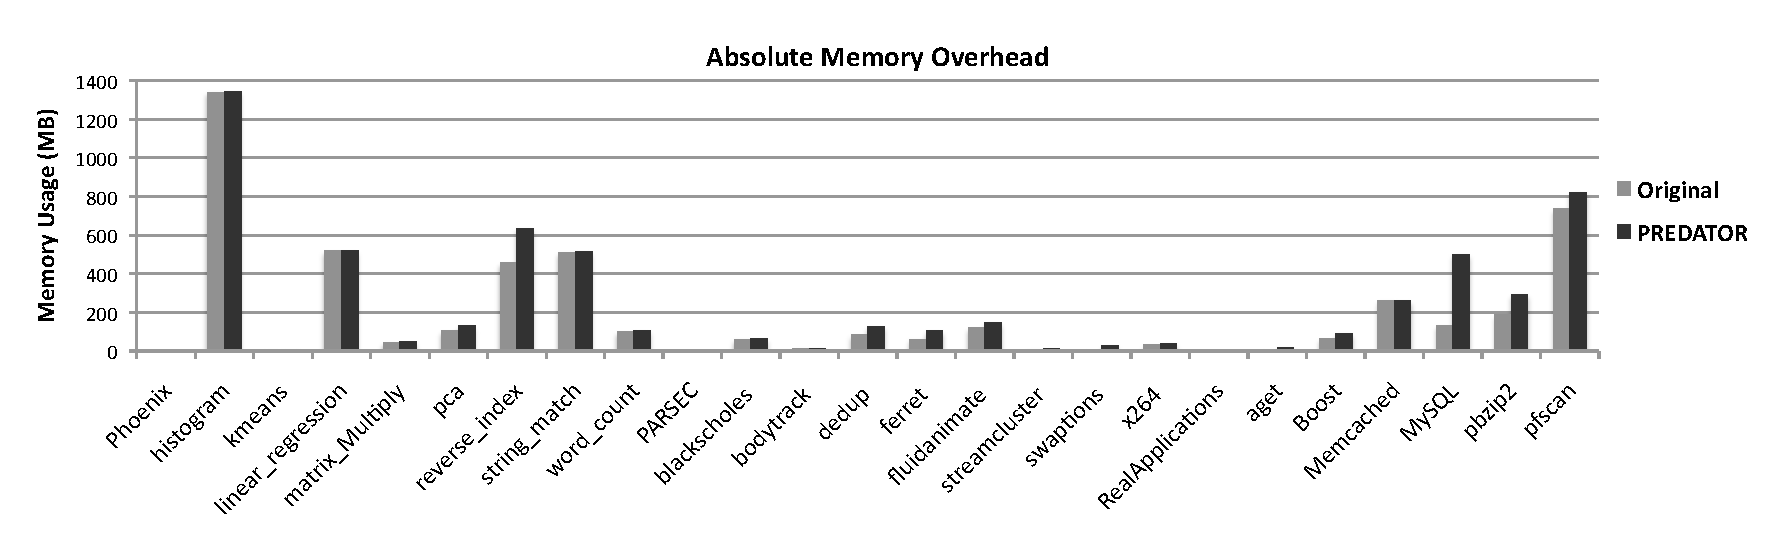
\includegraphics[width=6in]{predator/figure/absolutememory}
\caption{Absolute physical memory usage overhead with \Predator{}.}
\label{fig:absolutememusage}
\end{figure*}

\begin{figure*}[!t]
\centering
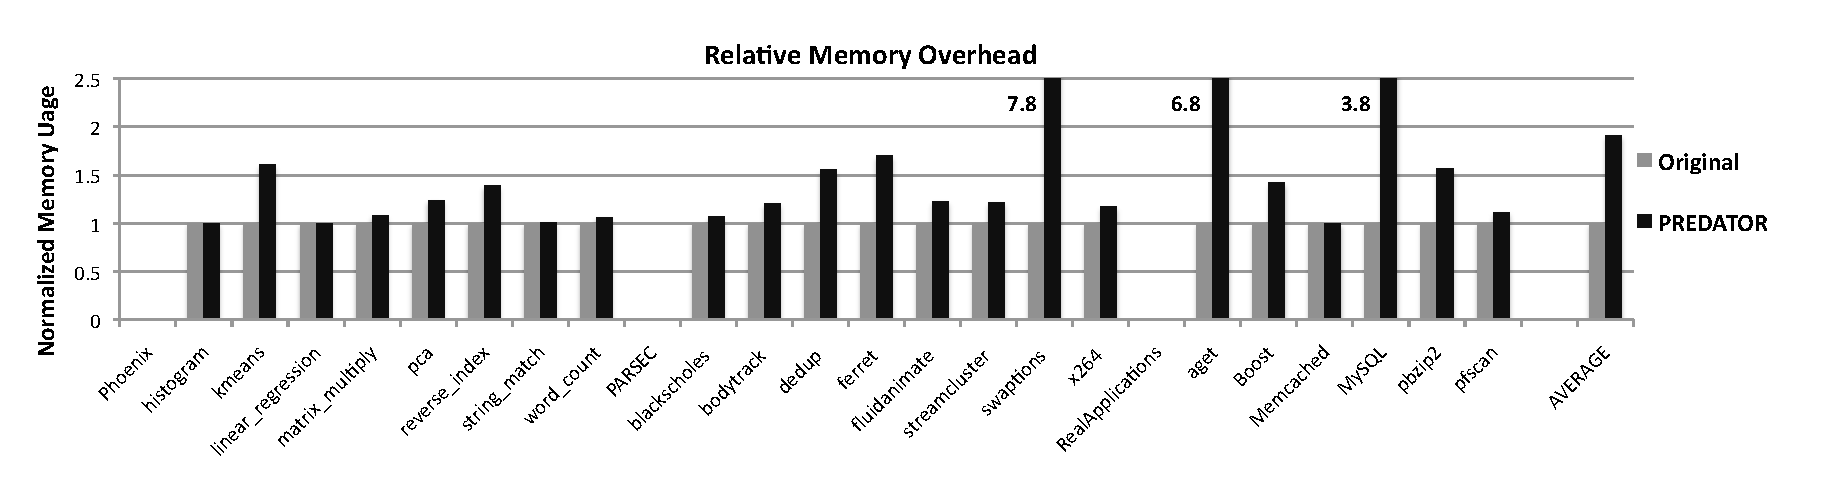
\includegraphics[width=6in]{predator/figure/memusage}
\caption{Relative physical memory usage overhead with \Predator{}.}
\label{fig:memusage}
\end{figure*}







%%
%% Beginning of back matter
\backmatter  %% <--- mandatory

%%
%% We don't support endnotes

%%
%% A bibliography is required.
\bibliographystyle{umthesis}
%\bibliography{dthreadsrefs}
%\bibliography{doubletakerefs}
%\bibliography{sheriffrefs}
\bibliography{refs}
\end{document}

%%% Local Variables: 
%%% mode: latex
%%% TeX-master: t
%%% End: 
